% --- Pass options before class loads
\PassOptionsToPackage{unicode,colorlinks,linkcolor=blue,citecolor=blue,urlcolor=blue}{hyperref}
\PassOptionsToPackage{dvipsnames}{xcolor}
\documentclass{iopjournal}

% --- Encoding, fonts, micro-typography
\usepackage[utf8]{inputenc}
\usepackage[T1]{fontenc}
\usepackage{lmodern}
\usepackage{microtype}
\emergencystretch=3em

% --- Script letters
\usepackage[scr=rsfso]{mathalpha}

% --- Math / figures / tables
\usepackage{amsmath,amssymb,amsfonts,amsthm,mathtools}
\usepackage{graphicx}
\graphicspath{{figures/}}
\graphicspath{{../figures/}}


\usepackage{tabularx,ragged2e,booktabs,float}
\newcolumntype{Y}{>{\RaggedRight\arraybackslash}X} % wrapped text column

% --- siunitx ↔ physics: warning-proof setup
% suppress the one-line siunitx message about `physics`
\ExplSyntaxOn
\msg_redirect_name:nnn { siunitx } { physics } { none }
\ExplSyntaxOff

% load siunitx first, then physics
\usepackage{siunitx}
\sisetup{
  detect-all,
  separate-uncertainty = true,
  per-mode = symbol,
  range-phrase = --,
}
\usepackage{physics}

% keep physics' \qty (for bracketed quantities) as \qtybr,
% and give \qty to siunitx (\SI)
\let\qtybr\qty
\makeatletter
\@ifundefined{RenewCommandCopy}{%
  \usepackage{letltxmacro}%
  \AtBeginDocument{\LetLtxMacro\qty\SI}%
}{%
  \AtBeginDocument{\RenewCommandCopy\qty\SI}%
}
\makeatother
% Now: \qty{3.2}{\metre\per\second} -> siunitx units; use \qtybr{...} for physics-style quantity brackets.

% --- Colored boxes
\usepackage[most]{tcolorbox}
\newtcolorbox{conceptbox}[1][]{%
  colback=blue!5!white,
  colframe=blue!75!black,
  fonttitle=\bfseries,
  title=#1,
  breakable, enhanced,
  boxrule=0.6pt,
  arc=2mm,
  left=1em, right=1em, top=0.6em, bottom=0.6em
}

% --- Misc helpers
\usepackage{braket}
\usepackage{enumitem}
\usepackage{float}

% --- Citations
\usepackage[numbers,sort&compress]{natbib}

% --- Cross-references (class loads hyperref; load cleveref after)
\usepackage[capitalise,nameinlink,noabbrev,sort&compress]{cleveref}
\crefname{equation}{Eq.}{Eqs.}
\Crefname{equation}{Equation}{Equations}
\crefname{figure}{Fig.}{Figs.}
\Crefname{figure}{Figure}{Figures}
\crefname{table}{Table}{Tables}
\Crefname{table}{Table}{Tables}
% Names for sections and appendices
\crefname{section}{Sec.}{Secs.}
\Crefname{section}{Section}{Sections}

\crefname{appendix}{Appendix}{Appendices}
\Crefname{appendix}{Appendix}{Appendices}

% (Optional) make multi-refs explicit; harmless on older cleveref
\crefmultiformat{section}
  {Secs.~#2#1#3}
  { and~#2#1#3}
  {, #2#1#3}
  { and~#2#1#3}

\crefmultiformat{appendix}
  {Appendix~#2#1#3}
  { and~#2#1#3}
  {, #2#1#3}
  { and~#2#1#3}








\begin{document}

\articletype{Article type} % e.g. Paper, Letter, Topical Review

\title{General Relativity as the Infrared EFT of a Proto-Field:\\ Induced Gravity, PN Equivalence, and Compact-Object Phenomenology}

\author{Moeidh Mana Hanash$^1$}

\affil{$^1$Independent Researcher}

\email{engmoeidh85@gmail.com}

\keywords{sample term, sample term, sample term}

\begin{abstract}
I formulate a concrete ``GR as induced IR–EFT’’ construction in which the effective geometry is a rank–one disformal update of Minkowski,
$g^{\rm eff}{\mu\nu}=\eta{\mu\nu}+\alpha,\partial_\mu\Phi,\partial_\nu\Phi$,
and the Einstein–Hilbert term arises at one loop on $(\mathcal M,g^{\rm eff})$. The induced coefficient is
$\frac{1}{16\pi G_{\rm ind}}=\frac{N_{\rm sp}\Lambda^2}{32\pi^2}\big(\xi_{\rm eff}+\frac{1}{6}\big)$
(minimal spectators: $\xi_{\rm eff}=0\Rightarrow\frac{1}{16\pi G_{\rm ind}}=\frac{N_{\rm sp}\Lambda^2}{192\pi^2}$); I adopt the minimal case unless stated otherwise. The $\Lambda^2$ term is scheme–dependent up to local counterterms, whereas the curvature–squared logarithms (and their nonlocal kernels) are universal. These logs fix finite range scales $(\ell_2,\ell_0)$ that enter only through $(1+\ell^2\Box)$ factors in the linearised operator. Under five explicit assumptions—(A1) no extra massless field, (A2) finite ranges $\ell_{2,0}$, (A3) asymptotic flatness with no incoming massive modes, (A4) slow–variation for the heat–kernel expansion, (A5) universal coupling to $g^{\rm eff}{\mu\nu}$—the operator factorises into GR times $(1+\ell^2\Box)$, and in the infrared window $k\ell{2,0}\ll1$ the theory is \emph{measurement–equivalent} to GR: the conservative PN sector matches through 2PN, the dissipative sector through 2.5PN (quadrupole flux), and there is no dipole channel.

For static, spherically symmetric C$^\prime$ backgrounds I solve $\nabla^2\Phi=4\pi,\zeta,\rho$ with $\Phi(\infty)=0$ to obtain a monotone lapse $N=e^{2\Phi}$ and use $A(r)=1+\alpha,\phi'(r)^{2}$ as a controlled interior weight. The photon–sphere condition is lapse–only ($rN'=2N$), yielding a phase boundary $\zeta_{\rm crit}=[\max_r M(r)/r]^{-1}$. As a result, the shadow diameter $\theta_{\rm sh}\simeq 2b_{\rm crit}/D_L$ depends only on $N$, while strong–lensing time delays and echo spacings depend on $\sqrt{A/N}$ and thus probe $\alpha$. In the eikonal ringdown, $\Omega_{\rm ph}=\sqrt{N}/r_{\rm ph}$ and $\Lambda_{\rm ph}=\sqrt{\big(2N-r^{2}N''\big)/(2A,r^{2})}$ (evaluated at $r_{\rm ph}$) separate lapse versus interior sensitivities.


For slow rotation I implement the Hartle–Thorne scheme with $j=(NA)^{-1/2}$ at $O(\Omega)$ and a stabilised interior/exterior match at $O(\Omega^2)$ to extract $(I,Q)$ and the invariants $(\bar I,\bar Q)$; in the minimal C$^\prime$ family the fitted quadrupole is prolate across the scanned compactness. The observational programme is therefore a joint–constraint triangle: \emph{shadow} fixes $\zeta$ (lapse), \emph{strong–lensing delay} fixes $\alpha$ (interior weight) at fixed $\zeta$, and \emph{inspiral phasing} bounds the mass–scaled $\alpha$ via the 2.5PN log. Within $r\gg\ell_{2,0}$ these tests over–constrain the model while preserving PN/PPN equivalence with GR.
\end{abstract}

\section{Introduction}\label{sec:intro}
General Relativity (GR) has withstood every precision test to date, from Solar–System dynamics and binary pulsars to gravitational–wave phasing \cite{Will2014LRR,PoissonWill2014,Blanchet2014LRR}. What GR does not answer is \emph{why} the Einstein–Hilbert (EH) action should govern the long–distance dynamics of spacetime, nor how that dynamics emerges from microphysics. Following the line opened by Sakharov—gravity as an induced phenomenon from quantum fluctuations of matter on a background geometry \cite{Sakharov1967,Visser2002}—I develop and test a concrete ``proto–field gravity model’’ (PFGM) in which an effective metric

\begin{equation}
g^{\rm eff}_{\mu\nu}=\eta_{\mu\nu}+\alpha\,\partial_\mu\Phi\,\partial_\nu\Phi
\label{eqn:01}
\end{equation}
is a rank–one disformal update of Minkowski. Because all metric dependence is \emph{algebraic} in $\partial\Phi$, the $\Phi$–equation is second order and the cone domain $1+\alpha X>0$ (with $X\equiv\eta^{\mu\nu}\partial_\mu\Phi\partial_\nu\Phi$) makes hyperbolicity transparent. A one–loop heat–kernel computation on $g^{\rm eff}$ induces an EH term with 
\begin{equation}
\dfrac{1}{16\pi G_{\rm ind}}=\dfrac{N\,\Lambda^2}{32\pi^2}\Big(\xi_{\rm eff}+\dfrac{1}{6}\Big), 
\qquad
\text{(minimal spectators: } \xi_{\rm eff}=0\ \Rightarrow\ \dfrac{1}{16\pi G_{\rm ind}}=\dfrac{N\,\Lambda^2}{192\pi^2}).
\label{eqn:02}
\end{equation}


In this notation $\xi_{\rm eff}$ summarises the spin/content–dependent endomorphism in the Laplace–type operator used in \cref{app:A}; minimally coupled scalars have $\xi_{\rm eff}=0$, while the universal $+\frac{1}{6}$ comes from the $a_1$ coefficient.
The usual curvature–squared logarithms \cite{DeWitt1965,BirrellDavies,ParkerToms,Vassilevich2003,BarvinskyVilkovisky,Donoghue1994}. I then show that, once short–range tails associated with those curvature–squared terms are parametrised by two length scales $\ell_{2}$ (spin–2) and $\ell_{0}$ (scalar), the long–distance dynamics of PFGM \emph{coincides} with GR to the Post–Newtonian (PN) orders probed experimentally.

\paragraph{Assumptions (A1–A5).}
I work under five mild, explicit assumptions referred to throughout the paper. (A1) There is no extra \emph{massless} propagating field beyond the emergent metric mode; all spectator excitations are gapped. (A2) The curvature–squared tail of the one–loop effective action is in the standard $C^2\!+\!R^2$ basis; its linearised ranges are finite and define $\ell_{2}$ and $\ell_{0}$ (\cref{app:A}). (A3) Asymptotic flatness holds and \emph{no incoming massive modes} are allowed in the boundary conditions (\cref{app:B4}). (A4) The heat–kernel/gradient expansion used to derive \eqref{eqn:02} is applied in its adiabatic/slow–variation regime \cite{ParkerToms,Vassilevich2003}. (A5) Matter couples universally to $g^{\rm eff}_{\mu\nu}$, so the weak and strong equivalence principles hold in the infrared (IR).

\begin{conceptbox}[Main claim]
	In the IR regime $r\gg \ell_{0,2}$ (equivalently $k\ell_{0,2}\ll1$), PFGM reproduces \emph{all} conservative PN predictions of GR through 2PN and the dissipative sector through 2.5PN, with the single replacement $G\to G_{\rm ind}$ defined in \eqref{eqn:02}. In particular the PPN parameters satisfy $\gamma=\beta=1$ through 2PN and the leading radiation–reaction term is the GR quadrupole at 2.5PN with no dipole channel \cite{Will2014LRR,PoissonWill2014,Blanchet2014LRR}.
	
\end{conceptbox}




The mechanism behind the boxed statement is simple: the curvature–squared sector factorises the linearised operator into GR times $(1+\ell^2\Box)$ in the spin–2 and spin–0 channels; at $k\ell\ll1$ these ``range operators’’ contribute only $\order{(\ell k)^2}$ corrections while the EH piece dominates. The absence of any additional long–range field (A1) forbids a dipole flux. I make these points precise in \crefrange{sec:linear}{sec:ppn} and \crefrange{app:B}{app:C}, and I exhibit the induced $G_{\rm ind}$ and range scales explicitly in \cref{sec:induced} and \cref{app:A}.


\paragraph{What is new here.}
Two ingredients distinguish my construction. First, the rank–one disformal algebra \eqref{eqn:01} keeps causality and second–order field equations manifest while allowing a controlled interior deviation ($A(r)\neq N(r)^{-1}$) in static, spherically symmetric spacetimes (``C$^\prime$’’ backgrounds; \cref{sec:model}, a regime that cleanly separates exterior observables set by $N$ from interior sensitivities that enter strong lensing and time delays through $\sqrt{A/N}$ (\cref{sec:geodesics,sec:delays}) \cite{Bekenstein1993,BettoniLiberati2013,Perlick2004LRR}. Second, in place of a full UV completion I give a minimal, regulator–explicit induction of the EH term (\cref{app:A}), treat the $C^2,R^2$ tails as an EFT remainder with ranges $\ell_{2,0}$, and show that \emph{all} current weak–field tests are passed in the IR window defined by those ranges.

\paragraph{Roadmap.}
Section (sec:model) introduces the PFGM and the C$^\prime$ ansatz. Section (sec:induced) sketches the one–loop induction of the EH term and defines $\ell_{0,2}$ via curvature–squared logs; details are in \cref{app:A}. Section (\cref{sec:linear}) derives the factorised linear operator and states the IR domain and boundary conditions (\cref{app:B}). Section (sec:ppn) proves PN/PPN equivalence through 2PN and the 2.5PN dissipative agreement (\cref{app:C}). Sections (\crefrange{sec:geodesics}{sec:delays}) develop null geodesics, strong lensing, and time delays on C$^\prime$ backgrounds, highlighting the complementary $N$–only vs.\ $(N,A)$ sensitivities (\crefrange{app:D}{app:G}). Sections (sec:tidal)–(sec:rotation) cover tides and slow rotation (Hartle–Thorne) and build the I–Love–Q panel; the $O(\Omega)$ and $O(\Omega^2)$ formalisms and stabilisers appear in \crefrange{app:H}{app:I}, and the Love–number machinery in \cref{app:J}. Data products, numerics, and error budgets are consolidated in \cref{app:K,app:L}, and conventions are in \cref{app:M}.

\medskip
Throughout I keep the notation and normalisations consistent with the PN literature \cite{PoissonWill2014,Blanchet2014LRR} and with standard heat–kernel references \cite{DeWitt1965,ParkerToms,Vassilevich2003}. 

\section{Proto–Field model and effective geometry}\label{sec:model}
\paragraph{Fields, coupling, and the effective metric.}
The proto–field gravity model (PFGM) has a single scalar ``proto–field’’ $\Phi$ and an \emph{effective} metric defined as a rank–one disformal update of Minkowski,
\begin{equation}
g^{\rm eff}_{\mu\nu}=\eta_{\mu\nu}+\alpha\,\partial_\mu\Phi\,\partial_\nu\Phi,
\qquad
X\equiv \eta^{\mu\nu}\partial_\mu\Phi\,\partial_\nu\Phi,
\label{eq:model_disformal}
\end{equation}
with inverse and determinant given by the Sherman–Morrison identities (\cref{app:M4}). The cone domain
$1+\alpha X>0$ ensures Lorentzian signature and invertibility; for static fields $X=|\nabla\Phi|^2\ge0$ so the condition reads $1+\alpha|\nabla\Phi|^2>0$ \cite{Bekenstein1993,BettoniLiberati2013}. Matter and any spectator species couple \emph{universally} to $g^{\rm eff}_{\mu\nu}$, so the equivalence principle holds in the IR. I keep the microscopic Lagrangian for $\Phi$ schematic—local in $\partial\Phi$ and compatible with \eqref{eq:model_disformal}—and use only its static limit (below) and the one–loop properties of the spectator sector.

\paragraph{One–loop induction and the spectator sector (summary).}
Integrating out $N_{\rm sp}$ spectator fields of Laplace type on $(\mathcal M,g^{\rm eff})$ induces an Einstein–Hilbert (EH) term and a curvature–squared tail (\cref{app:A}). Denoting by $\Lambda$ the proper–time cutoff, and by $\xi_{\rm eff}$ the spin/content–averaged nonminimal coupling in the endomorphism of the spectator operator (\cref{app:A1}), the induced EH coefficient is
\begin{equation}
\frac{1}{16\pi G_{\rm ind}}=\frac{N_{\rm sp}\,\Lambda^2}{32\pi^2}\Big(\xi_{\rm eff}+\tfrac{1}{6}\Big),
\qquad
\text{(minimal spectators: }\xi_{\rm eff}=0\Rightarrow \tfrac{1}{16\pi G_{\rm ind}}=\tfrac{N_{\rm sp}\Lambda^2}{192\pi^2}\text{)},
\label{eq:model_Gind_repeat}
\end{equation}
and the curvature–squared logarithms define finite linearised ranges $\ell_2$ (spin–2) and $\ell_0$ (spin–0) (\cref{app:A4,app:A5}) \cite{DeWitt1965,ParkerToms,Vassilevich2003,BarvinskyVilkovisky,Donoghue1994}. Throughout I distinguish the \emph{lapse} $N(r)$ of \eqref{eq:model_Cprime} below from the spectator count $N_{\rm sp}$ in \eqref{eq:model_Gind_repeat}.
\noindent\emph{Scheme note.} The $\Lambda^2$ term in \eqref{eq:model_Gind_repeat} is regulator–dependent at the level of local counterterms, whereas the curvature–squared logarithms (and their nonlocal kernels) are universal (\cref{app:A3}). In what follows I adopt the \emph{minimal} case $\xi_{\rm eff}=0$ unless otherwise stated, so that $1/(16\pi G_{\rm ind})=N_{\rm sp}\Lambda^2/(192\pi^2)$, and absorb any scheme dependence into the renormalised $1/G$ at the matching scale.


\section{One–loop induced gravity and EFT tail}\label{sec:induced}
\paragraph{Heat–kernel outline (details in \cref{app:A}).}
For a set of $N_{\rm sp}$ spectator fields of Laplace type on $(\mathcal M,g^{\rm eff})$, the one–loop effective action in the proper–time scheme reads
\begin{equation}
\Gamma^{(1)}=\frac{1}{2}\sum_{a=1}^{N_{\rm sp}}\ln\det\mathcal P_a
=\frac{1}{32\pi^2}\!\int\! d^4x\sqrt{-g_{\rm eff}}\Big[\tfrac12\Lambda^4 a_0+\Lambda^2 a_1+\ln\!\Big(\frac{\Lambda^2}{\mu^2}\Big)a_2\Big]
+\Gamma^{(1)}_{\rm nonloc}+{\rm finite},
\label{eq:sec3_Gamma_loc}
\end{equation}
where $\mathcal P=-\Box_{g^{\rm eff}}+\mathcal E$ is of Laplace type, and $a_0=\mathbf{1}$, $a_1=\mathcal E+\tfrac16 R$, while $a_2$ is the usual local quadratic curvature combination (\cref{app:A2}) \cite{DeWitt1965,BirrellDavies,ParkerToms,Vassilevich2003}. Euclidean continuation is understood; signs match my Lorentzian convention via $\mathcal P=-\Box+\mathcal E$. The nonlocal piece has the universal Barvinsky–Vilkovisky form
\begin{equation}
\Gamma^{(1)}_{\rm nonloc}
=\frac{1}{32\pi^2}\!\int\! \sqrt{-g_{\rm eff}}\Big[
c_C\,C_{\mu\nu\rho\sigma}\ln\!\Big(\frac{-\Box_{g_{\rm eff}}}{\mu^2}\Big)C^{\mu\nu\rho\sigma}
+c_R\,R\,\ln\!\Big(\frac{-\Box_{g_{\rm eff}}}{\mu^2}\Big)R+\cdots\Big],
\label{eq:sec3_nonloc}
\end{equation}
with $c_{C,R}$ fixed by $a_2$ \cite{BarvinskyVilkovisky,BarvinskyVilkovisky1990,Donoghue1994}.

\paragraph{Induced Einstein–Hilbert coefficient (boxed).}
Matching the $\Lambda^2 a_1$ term to the Einstein–Hilbert action gives
\begin{equation}
\boxed{\frac{1}{16\pi G_{\rm ind}}=\frac{N_{\rm sp}\Lambda^2}{32\pi^2}\Big(\xi_{\rm eff}+\tfrac16\Big),
\qquad
\text{minimal spectators: }\xi_{\rm eff}=0\ \Rightarrow\ \frac{1}{16\pi G_{\rm ind}}=\frac{N_{\rm sp}\Lambda^2}{192\pi^2}.}
\label{eq:sec3_Gind_box}
\end{equation}

Here $\xi_{\rm eff}$ summarises the spin/content–dependent endomorphism in $\mathcal E$ (\cref{app:A1}); the universal $+\tfrac16$ comes from $a_1$ \cite{ParkerToms,Vassilevich2003}. \emph{Scheme note:} the $\Lambda^2$ coefficient is regulator–dependent up to local counterterms, whereas the quadratic–curvature logarithms (and their nonlocal kernels) are universal (\cref{app:A3}). In what follows I use the minimal case $\xi_{\rm eff}=0$ unless stated otherwise and absorb scheme dependence into the renormalised $1/G$ at matching.

\paragraph{Vacuum energy and scheme dependence.}
The $a_0$ piece gives a cosmological–constant term $\Delta\mathcal L_{\Lambda^4}=N_{\rm sp}\Lambda^4/(64\pi^2)$ (per real scalar), and massive spectators contribute an additional $m^4\ln(\Lambda^2/\mu^2)/(64\pi^2)$ inside \eqref{eq:sec3_Gamma_loc}. Both are absorbed into the renormalised vacuum energy at the matching scale; their precise values are scheme choices \cite{ParkerToms}.

\paragraph{Curvature–squared logs and ranges.}
Writing the logarithmic local part in the $\{C^2,E_4,R^2\}$ basis,
\begin{equation}
\Gamma^{(1)}_{\rm log}
=\frac{1}{32\pi^2}\ln\!\Big(\frac{\Lambda^2}{\mu^2}\Big)\!\int\!\sqrt{-g_{\rm eff}}\,
\big[c_C\,C^2-c_E\,E_4+c_R\,R^2+\cdots\big],
\label{eq:sec3_logs}
\end{equation}
one has for a single minimally coupled scalar $c_C=\tfrac{1}{120}$,\ $c_E=\tfrac{1}{360}$,\ $c_R=\tfrac{1}{72}\ \big(\text{and }c_R=\tfrac12(\xi-\tfrac16)^2$ at general $\xi\big)$ so $a_2=\tfrac{1}{120}C^2-\tfrac{1}{360}E_4+\tfrac{1}{72}R^2+\cdots$\ and $E_4$ is topological in $d=4$ (no local dynamics). $\xi$; \cref{app:A2}). Promoting $\mu$ to a running scale and combining \eqref{eq:sec3_nonloc} with local counterterms leads to the effective quadratic action with \emph{finite} couplings $\alpha_C(\mu)$ and $\alpha_R(\mu)$. The corresponding \emph{range scales} in the linearised theory are (\cref{app:A5})
\begin{equation}
\ell_2^{\,2}=32\pi G(\mu)\Big[\alpha_C(\mu)+\frac{c_C}{32\pi^2}\ln\!\frac{\mu_*^2}{\mu^2}\Big],\qquad
\ell_0^{\,2}=96\pi G(\mu)\Big[\alpha_R(\mu)+\frac{c_R}{32\pi^2}\ln\!\frac{\mu_*^2}{\mu^2}\Big],
\label{eq:sec3_ranges}
\end{equation}
so that the linearised operator factorises as $\bar\Box\,(1+\ell_2^2\bar\Box)$ in the spin–2 sector and $\bar\Box\,(1+\ell_0^2\bar\Box)$ in the spin–0 sector (\cref{app:B1}). Heuristically, at fixed $\mu$ one may read $\ell_2^{\,2}\sim G_{\rm ind}\,c_C$ and $\ell_0^{\,2}\sim G_{\rm ind}\,c_R$.


\paragraph{EFT window and ``ghost’’ decoupling.}
The quadratic–curvature sector introduces massive poles at $m_2^{-2}=\ell_2^{\,2}$ and $m_0^{-2}=\ell_0^{\,2}$ in the respective propagators (\cref{app:B5}). In a purely local $C^2+R^2$ theory the spin–2 pole carries the well–known ghostlike sign \cite{Stelle1977}; in my EFT this is immaterial provided I restrict to the IR window
\begin{equation}
k\ell_{2,0}\ll1,\qquad r\gg \ell_{2,0},
\label{eq:sec3_IRwindow}
\end{equation}
and impose \emph{no incoming massive modes} in the boundary conditions (\cref{app:B4}). In this regime the curvature–squared sector contributes only $\order{(\ell_{2,0}k)^2}$ corrections, the nonlocal kernels reduce to mild logarithms, and GR with $G\to G_{\rm ind}$ emerges as the universal IR limit (\cref{app:B6}/\cref{app:C3}). Any potential pathologies at the heavy poles lie outside the EFT domain and are not excited by admissible initial/boundary data.

\paragraph{Summary for later use.}
(i) The EH coefficient is set by \eqref{eq:sec3_Gind_box} with the minimal choice $\xi_{\rm eff}=0$ used in my numerics; (ii) the only new IR parameters are the ranges $\ell_{2,0}$ in \eqref{eq:sec3_ranges}; (iii) all weak–field/PPN observables coincide with GR through 2PN (conservative) and 2.5PN (dissipative), with corrections suppressed by $(\ell_{2,0}k)^2$ under the boundary conditions stated above. I use these facts in \crefrange{sec:linear}{sec:ppn} and build the null–geodesic and compact–object phenomenology in \crefrange{sec:geodesics}{sec:rotation}.

\section{Linearized dynamics, range, and boundary conditions}\label{sec:linear}
\paragraph{Factorised linear operator and ranges.}
Linearising the equations about an asymptotically flat background (\cref{app:B}) and working in harmonic gauge, the metric perturbation $h_{\mu\nu}$ decomposed with the Barnes–Rivers projectors satisfies a \emph{factorised} fourth–order system in each physical sector:
\begin{equation}
\mathcal{E}\,h
=-\tfrac12\Big[(1+\ell_2^{\,2}\Box)\,\Box\,P^{(2)}+(1+\ell_0^{\,2}\Box)\,\Box\,P^{(0{\rm s})}\Big]\,h
=-16\pi G(\mu)\,\mathcal S,
\label{eq:lin_factor}
\end{equation}
Here $\mathcal E$ denotes the linearised Euler–Lagrange operator on $h_{\mu\nu}$ in harmonic gauge, and $\mathcal S$ is the corresponding projected source; indices are suppressed by the Barnes–Rivers projectors.
 $\mathcal S$ denotes the projected source, and the range scales are those fixed by the curvature–squared tail (\cref{app:A5}),
\begin{equation}
\ell_2^{\,2}=32\pi G(\mu)\Big[\alpha_C(\mu)+\tfrac{c_C}{32\pi^2}\ln(\mu_*^2/\mu^2)\Big],\qquad
\ell_0^{\,2}=96\pi G(\mu)\Big[\alpha_R(\mu)+\tfrac{c_R}{32\pi^2}\ln(\mu_*^2/\mu^2)\Big].
\label{eq:lin_ranges}
\end{equation}
Equivalently, the full (factorised) characteristic polynomial in local Fourier space is
$\tfrac12\,\xi^2(1-\ell_2^{\,2}\xi^2)P^{(2)}+\tfrac12\,\xi^2(1-\ell_0^{\,2}\xi^2)P^{(0{\rm s})}$, i.e.\ the union of the GR light cone $\{\xi^2=0\}$ and massive cones $\{\xi^2=\ell_{2,0}^{-2}\}$ (\cref{app:B1}). The principal symbol (degree–4 part) follows by keeping only the $\xi^4$ coefficients. In the cone domain $1+\alpha X>0$ the system is the product of two normally hyperbolic second–order operators and is therefore \emph{strongly hyperbolic} (\cref{app:B1}).

\paragraph{Boundary conditions.}
I impose asymptotic flatness and rule out incoming massive modes (\cref{app:B4}). In the massless spin–2 sector one selects the retarded Green function by the Sommerfeld condition,
\begin{equation}
\lim_{r\to\infty} r(\partial_t+\partial_r)h^{(2)}_{\rm TT}=0,
\label{eq:lin_bc_massless}
\end{equation}
while in the massive branches one imposes \emph{no incoming massive modes}. In the IR regime $\omega\ell_{2,0}\ll1$ these branches are evanescent and decay as $e^{-r/\ell_{2,0}}$; if a frequency component satisfies $\omega>\ell^{-1}$ (outside the EFT window), one uses the massive Sommerfeld condition $\lim_{r\to\infty}r(\partial_r-i q)h_{\rm m}=0$ with $q=\sqrt{\omega^2-\ell_{2,0}^{-2}}$ and branch $\Re q\ge0$ (\cref{app:B4}).

\paragraph{IR domain and equivalence.}
In the \emph{infrared} window
\begin{equation}
k\ell_{2,0}\ll1\qquad\Longleftrightarrow\qquad r\gg \ell_{2,0},
\label{eq:lin_IRwindow}
\end{equation}
the inverse of the factorised operator admits the Neumann expansion
\[
\frac{1}{(1+\ell^2\Box)\,\Box}=\frac{1}{\Box}\Big(1-\ell^2\Box+\order{\ell^4\Box^2}\Big),
\]
so that the linear response reduces to that of GR with $G\to G(\mu)=G_{\rm ind}$ up to $\order{(\ell_{2,0}k)^2}$ corrections (\cref{app:B6}). Concretely,
\begin{equation}
h_{\mu\nu}=h_{\mu\nu}^{\rm GR}\Big[1+\order{(\ell_{2,0}k)^2}\Big],\qquad
\text{with}\ \ h_{\mu\nu}^{\rm GR}=-\frac{16\pi G(\mu)}{\Box}\,\mathcal S_{\mu\nu},
\label{eq:lin_equivalence}
\end{equation}
and all PPN observables coincide with GR through 2PN in the conservative sector and 2.5PN in the dissipative sector under the boundary conditions above (\cref{app:C}; \cite{PoissonWill2014,Will2014LRR,Blanchet2014LRR}). Corrections from the curvature–squared tail enter at $\order{(\ell_{2,0}k)^2}$ and are negligible in this domain.

\section{Post–Newtonian/PPN equivalence in the IR}\label{sec:ppn}
\paragraph{Poisson hierarchy with $G\to G_{\rm ind}$.}
In the near zone I work in harmonic gauge and expand the metric in PN orders,
\[
g_{00}=-1+h_{00}^{(2)}+h_{00}^{(4)}+\order{\varepsilon^{6}},\quad
g_{0i}=h_{0i}^{(3)}+h_{0i}^{(5)}+\order{\varepsilon^{7}},\quad
g_{ij}=\delta_{ij}+h_{ij}^{(2)}+h_{ij}^{(4)}+\order{\varepsilon^{6}},
\]
with $\varepsilon\sim v\sim\sqrt{GM/r}\ll1$ (\cref{app:C1}; \cite{PoissonWill2014,Blanchet2014LRR}). In the IR window $k\ell_{0,2}\ll1$ (\cref{sec:linear}) the linearised operator factorises and its inverse admits the Neumann expansion; the field equations reduce, order by order, to the \emph{GR} Poisson hierarchy with the replacement $G\to G(\mu)\equiv G_{\rm ind}$:
\begin{align}
\nabla^2 U(\boldsymbol x,t)&=-4\pi G(\mu)\,\rho(\boldsymbol x,t), &
\nabla^2 V_i(\boldsymbol x,t)&=-4\pi G(\mu)\,\rho v_i, \label{eq:ppn_Poisson1}\\
\nabla^2 \Phi_1&=-4\pi G(\mu)\,\rho v^2, &
\nabla^2 \Phi_2&=-4\pi G(\mu)\,\rho U, \\
\nabla^2 \Phi_3&=-4\pi G(\mu)\,\rho \Pi, &
\nabla^2 \Phi_4&=-4\pi G(\mu)\,p, \label{eq:ppn_Poisson2}
\end{align}
together with $\nabla^2 X=-2U$ and the standard near–zone integrals (\cref{app:C2}). Terms proportional to $\Box R$ in the one–loop $a_2$ coefficient are \emph{local total derivatives} and, in the PN matching, can be absorbed into boundary terms; they do not alter the local PPN potentials \cite{ParkerToms,Vassilevich2003}.

\paragraph{Boxed result (metric to 2PN).}
Assembling the PN metric from \eqref{eq:ppn_Poisson1}–\eqref{eq:ppn_Poisson2} one finds exactly the GR expressions through 2PN with $G\to G(\mu)$ (\cref{app:C3}):
\[
\boxed{\gamma=\beta=1\quad\text{through 2PN,}}
\]
under assumptions A1–A5 (no extra massless field; finite ranges $\ell_{0,2}$; asymptotic flatness with no incoming massive modes; slow–variation for the heat kernel; universal coupling to $g^{\rm eff}_{\mu\nu}$).

Concretely, in harmonic coordinates the 1PN line element has the standard form
\[
g_{00}=-1+2U-2U^2+2\Phi_1+2\Phi_2+2\Phi_3+2\Phi_4+\order{\varepsilon^{6}},\quad
g_{ij}=\delta_{ij}(1+2U)+\order{\varepsilon^{4}},
\]
with the coefficients unchanged from GR (\cref{app:C}; \cite{PoissonWill2014,Blanchet2014LRR}).

\paragraph{Dissipative sector and the absence of a dipole channel.}
In the IR limit the radiative kernel is the GR one (\cref{sec:linear}, \cref{app:B6}), so the leading reaction term enters at 2.5PN via the quadrupole flux \cite{Blanchet2014LRR}. A $(-1)$PN \emph{dipole} requires a long–range extra mode and non–universal couplings. Assumptions A1 and A5 forbid both: there is no additional massless field in the spectrum and all matter couples to the same $g^{\rm eff}_{\mu\nu}$. Hence no dipole channel is available and the dissipative sector matches GR at 2.5PN. In the SPA phasing convention this corresponds to a 2.5PN logarithmic term with fractional deviation $\delta\hat\phi_{5\ell}=\widehat\alpha$ at leading order in the minimal model (\cref{app:E2}).

\paragraph{Measurement equivalence (Solar System and pulsars).}
The statements above imply \emph{measurement equivalence} with GR for all weak–field tests performed within the IR domain: light deflection and Shapiro delay (Cassini) probe $\gamma$ and are saturated by $\gamma=1$; perihelion/periastron advances and Nordtvedt–type tests probe $\beta$ and yield $\beta=1$; binary–pulsar timing and early inspiral phasing probe the 2.5PN reaction term and see the GR quadrupole without a dipole channel \cite{Will2014LRR,PoissonWill2014,Blanchet2014LRR,BertottiIessTortora2003}. Any residual corrections from the curvature–squared tail scale as $(\ell_{0,2}k)^2$ and are negligible provided the observational scales $r$ satisfy $r\gg \ell_{0,2}$ and the boundary conditions exclude incoming massive modes (\crefrange{app:B4}{app:B6}).

\paragraph{Scope of the equivalence.}
The boxed result holds for the conservative sector through 2PN and the dissipative sector at 2.5PN; the first new conservative sources allowed by the rank–one disformal algebra appear at 3PN (and then 4PN) via gradients of $U$ (\cref{app:C5}). Those higher–order effects are beyond current Solar–System precision and enter gravitational–wave phasing at orders subleading to the quadrupole log; I parameterise them explicitly in \cref{app:E} and use them in \cref{sec:phasing} for bounds on $\widehat\alpha$ from inspiral data.
I impose near–zone boundary conditions $U,V_i,\Phi_A\to 0$ as $r\to\infty$ (asymptotic flatness with no incoming massive modes), so the Poisson problems \eqref{eq:ppn_Poisson1}–\eqref{eq:ppn_Poisson2} have unique solutions given by the standard instantaneous integrals (\cref{app:C2}).
In the static limit $\Box\to\nabla^{2}$ the range operators appear as $(1+\ell_{2,0}^{\,2}\nabla^{2})\nabla^{2}$, so all range corrections enter with the same $+\ell^{2}\nabla^{2}$ sign used in \cref{app:C}.

\section{GW inspiral phasing handle}\label{sec:phasing}
\paragraph{SPA phase and my normalisation.}
For quasi–circular binaries the frequency–domain strain is well described by the stationary–phase approximation (SPA) \cite{CutlerFlanagan1994,SathyaprakashSchutz2009,Blanchet2014LRR}. With $v=(\pi GM f/c^{3})^{1/3}$ and symmetric mass ratio $\eta$, the GR phase reads
\begin{equation}
\Psi_{\rm GR}(f)=2\pi f t_c-\phi_c-\frac{\pi}{4}
+\frac{3}{128\,\eta}\,v^{-5}\!\left[1+\sum_{n\ge2}\varphi_n v^{n}+\sum_{n\ge5}\varphi_{n\ell} v^{n}\ln v\right],
\label{eq:phasing_GR}
\end{equation}
where the first logarithm arises at 2.5PN ($n=5$) from tails. In PFGM, the leading IR deformation appears as a \emph{single} dimensionless knob
\begin{equation}
\widehat\alpha\;\equiv\;\alpha\,\frac{c^{4}}{G^{2}M^{2}},
\label{eq:phasing_alpha_hat}
\end{equation}
multiplying the 2.5PN log piece at leading order (minimal model), with subleading conservative inserts at 3PN and 4PN (\cref{app:E2,app:E3}). I therefore write
\begin{equation}
\Delta\Psi(f)
= \frac{3}{128\,\eta}\,v^{-5}\,\widehat{\alpha}
\bigl[\kappa_{2.5}\,v^{5}\ln v+\kappa_{3}\,v^{6}+\kappa_{4}\,v^{8}+\order{v^{10}}\bigr],
\label{eq:phasing_template}
\end{equation}

with $\kappa_{2.5}=1$ at leading order in the minimal PFGM, and $(\kappa_{3},\kappa_{4})$ fixed by the near–zone energy inserts via the linear maps described in \cref{app:E3}. Equation \eqref{eq:phasing_template} is the template used to confront data; it reduces to the LVK ``parametrized tests” convention by identifying the fractional deviation of the 2.5PN–log coefficient,
\begin{equation}
\boxed{\ \delta\hat\phi_{5\ell}=\kappa_{2.5}\,\widehat\alpha\ } ,
\label{eq:phasing_map_delta}
\end{equation}
so that $\delta\hat\phi_{5\ell}=\widehat\alpha$ in the minimal choice $\kappa_{2.5}=1$ (\cref{app:E2}).
\noindent\emph{LVK convention.} In parametrized tests the GR $2.5$PN--log coefficient $\varphi_{5\ell}^{\rm GR}(\eta)$ is multiplied by $(1+\delta\hat\phi_{5\ell})$ while all other PN coefficients are kept at their GR values; \eqref{eq:phasing_map_delta} implements precisely this replacement for my template.


\begin{figure}[t]
\centering
\includegraphics[width=0.8\linewidth]{alpha_max_vs_x_mass_dependent.png}
\caption{Bound scaling for \(\alpha\) from the 2.5PN log phasing test (\(\delta\hat\phi_{5\ell}=\kappa_{2.5}\widehat\alpha\)). Curves show \(\alpha_{\max}(x)\) for representative masses (assumed \(\kappa_{2.5}=1\) at leading order; see \cref{app:E2}).}
\label{fig:alpha-mass-scaling}
\end{figure}

\paragraph{Event–level bounds and mass scaling.}
Given a per–event constraint on $\delta\hat\phi_{5\ell}$, the implied bound on $\alpha$ follows from \eqref{eq:phasing_alpha_hat}–\eqref{eq:phasing_map_delta}:
\begin{equation}
\boxed{\alpha_{90}\;=\;\frac{|\delta\hat\phi_{5\ell}|_{90}}{\kappa_{2.5}}\;\frac{G^{2}M^{2}}{c^{4}},
\qquad
M\ \text{in the \emph{source} frame,}\ \ M=\frac{M_{\rm det}}{1+z}.}
\label{eq:phasing_alpha_bound}
\end{equation}

Thus bounds scale as $M^{2}$ at fixed $|\delta\hat\phi_{5\ell}|_{90}$; I compute them using the source–frame masses in the CSVs and, when stacking events, combine $\delta\hat\phi_{5\ell}$ by inverse–variance weighting (\cref{app:E4,app:E5}). When non–minimal normalisations are used, the same formula applies with the recorded $\kappa_{2.5}$ for that analysis.
\noindent\emph{Mass choice.} The mapping \eqref{eq:phasing_alpha_bound} uses the source-frame total mass $M$ for equal-mass calibrations; for unequal masses one may equivalently scale $\widehat\alpha$ with the chirp mass $\mathcal M=\eta^{3/5}M$ without changing the procedure (the bound rescales accordingly with the mass used).

\paragraph{Including conservative 3PN/4PN inserts (nuisance or profiling).}
If desired, one may include the $\kappa_{3}v^{6}$ and $\kappa_{4}v^{8}$ pieces in \eqref{eq:phasing_template}. At fixed $(M,\eta)$ the phase remains \emph{linear} in $\widehat\alpha$, so limits derived from the 2.5PN log survive provided the higher–order pieces lie below statistical/systematic errors across the analysis band. my CSVs carry $(\kappa_{3},\kappa_{4})$ computed from the chosen $(C_{3},C_{4})$ (\cref{app:E3}); a conservative option is to profile over $(\kappa_{3},\kappa_{4})$ with Gaussian priors centred at the theory values and add the induced spread to the quoted $\alpha$ bound (\cref{app:E5}).

\paragraph{LVK and pulsar inputs; $(\alpha,\zeta)$ complementarity.}
LVK ``parametrized tests” provide event–level $\delta\hat\phi_{5\ell}$ constraints; applying \eqref{eq:phasing_alpha_bound} gives $(\alpha,M)$ bounds immediately. Binary–pulsar timing constrains the dissipative sector through the agreement of orbital decay with the GR quadrupole flux; in my model the leading reactive term is the 2.5PN quadrupole with \emph{no} dipole channel, so pulsars are consistent with $\delta\hat\phi_{5\ell}=0$ and bound $\widehat\alpha$ in the same way once mapped to an effective $\delta\hat\phi_{5\ell}$ (\cref{app:E5}). Phasing alone is insensitive to the interior lapse dial $\zeta$; to constrain $(\alpha,\zeta)$ jointly I combine \eqref{eq:phasing_alpha_bound} with shadow and strong–lensing time–delay data, which probe $N$ and $(N,A)$, respectively, and break the $(\alpha,\zeta)$ degeneracy (\cref{sec:geodesics,sec:delays,sec:obs}).

\paragraph{Practical use (CSV columns).}
The per–event CSVs list $\{\texttt{M\_source},\eta,z; \delta\hat\phi_{5\ell}\ \text{median}\pm90\%\}$ and the template coefficients $(\kappa_{2.5},\kappa_{3},\kappa_{4})$ (\cref{app:E4}). The column \texttt{alpha\_90} is computed by \eqref{eq:phasing_alpha_bound}; stacked bounds reported in the ``combined’’ CSV use inverse–variance weights on $\delta\hat\phi_{5\ell}$ with masses redshift–corrected to the source frame. For completeness I also provide templates with $(\kappa_{3},\kappa_{4})$ set to zero (pure 2.5PN–log deformation) and with their theory values (minimal profiling choice), so that either convention can be adopted without re–running the mapping (\cref{app:E5}).

\paragraph{Scope and limitations.}
Equation \eqref{eq:phasing_template} is valid in the inspiral regime where the SPA holds and $k\ell_{2,0}\ll1$; merger/ringdown and very high–frequency data lie outside my EFT window and are not used for $\alpha$ bounds. Within this scope, \eqref{eq:phasing_alpha_bound} is the direct route from LVK/pulsar summaries to $(\alpha,M)$ (or, in joint analyses with lensing, to $(\alpha,\zeta)$), and is the convention used in all bounds quoted in \cref{sec:obs}.

\section{\texorpdfstring{Static C$^\prime$ spacetimes: construction and scaling}{Static C' spacetimes: construction and scaling}}\label{sec:static}
\paragraph{Lapse solve and monotonicity.}
In the static sector the lapse is $N(r)=e^{2\Phi(r)}$ with $\Phi$ solving the Poisson problem
\begin{equation}
\nabla^2\Phi(r)=\frac{1}{r^2}\frac{d}{dr}\!\Big(r^2\Phi'(r)\Big)=4\pi\,\zeta\,\rho(r),
\qquad
\Phi(\infty)=0,
\label{eq:7_Poisson}
\end{equation}
for a non–negative source profile $\rho(r)$ and a dimensionless \emph{lapse dial} $\zeta>0$ (\cref{app:F1}). Gauss’ law gives the identity
\begin{equation}
r^{2}\Phi'(r)=\zeta\,M(r),\qquad
M(r)=4\pi\!\int_{0}^{r}\rho(\tilde r)\,\tilde r^{2}\,d\tilde r,
\label{eq:7_flux}
\end{equation}
so $\Phi'(r)\ge0$ and the lapse is monotone:
\begin{equation}
\Phi(r)\le0,\qquad N(r)=e^{2\Phi(r)}\le1,\qquad N'(r)=2\Phi'(r)\,N(r)\ge0,
\label{eq:7_monotone}
\end{equation}
with $N(r)\nearrow1$ as $r\to\infty$ (\cref{app:F1,app:F2}). For compact support $\rho(r>R_\ast)=0$, the exterior solution is
\begin{equation}
\Phi(r)=-\,\zeta\,\frac{M(R_\ast)}{r},\qquad
N(r)=\exp\!\Big[-\,\frac{2\zeta\,M(R_\ast)}{r}\Big],\qquad r\ge R_\ast.
\label{eq:7_ext}
\end{equation}
The photon–sphere condition depends only on $N$:
$r\,N'(r)=2N(r)\ \Leftrightarrow\ r\,\Phi'(r)=1$ (\cref{app:D3}/\cref{app:F2}).

\paragraph{Interior weight and the core scalar.}
I parameterise the interior metric weight by
\begin{equation}
A(r)=1+\alpha\,\phi'(r)^{2},
\label{eq:7_A_def}
\end{equation}
where $\phi(r)$ is a smooth core scalar profile (algebraically tied to $\partial\Phi$ in model realisations) supported primarily in the matter region. With $\alpha>0$ one has $A\ge1$ and the cone domain $1+\alpha X>0$ is manifest (\cref{app:M4}). Asymptotic flatness requires $\phi'\to0$ so that $A\to1$ at large $r$ (For $\alpha<0$ the cone condition $1+\alpha X>0$ restricts $|\nabla\Phi|$, and I keep $\alpha>0$ in the static backgrounds considered here.). Exterior null geodesics and shadow sizes depend on $N$ alone, whereas finite–$b$ deflections and time delays depend on both $N$ and $A$ through the optical metric $\sqrt{A/N}$ (\crefrange{app:D}{app:G}).



\paragraph{Surface proxies and $R_{90}$/$R_{95}$.}
To anchor interior/exterior matches and read–offs I define the \emph{mass–fraction radii} $R_f$ by
\begin{equation}
M(R_f)=f\,M(R_{\rm out}),\qquad f\in(0,1),\quad R_{\rm out}\gg R_f.
\label{eq:7_Rf}
\end{equation}
my baseline surface proxy is $R\equiv R_{90}$ ($f=0.90$); a value–weighted variant uses $R_{95}$ ($f=0.95$). The two choices are propagated through the Hartle/ Love pipelines (\crefrange{app:H}{app:J}), and their spread enters the error budget; in particular, a $\pm3\%$ shift in $R$ induces a $\pm15\%$ shift in $\bar\lambda$ at leading order (\cref{app:K3}).

\paragraph{Scaling to physical units.}
I work in dimensionless code units tied to a single length scale $r_0$ and restore dimensions at the end. A convenient choice is
\begin{equation}
r_0\ \equiv\ \zeta\,M(R_{\rm out}),
\label{eq:7_r0_def}
\end{equation}
so that the exterior solution \eqref{eq:7_ext} becomes $\Phi(x)=-1/x$ with $x=r/r_0$ and $N(x)=\exp[-2/x]$. Dimensionless variables are
\[
x\equiv \frac{r}{r_0},\qquad
\hat\rho(x)\;\equiv\;4\pi\,\zeta\,r_0^{2}\,\rho(r),
\]
so that \eqref{eq:7_Poisson} reads simply $\hat\nabla^{2}\Phi=\hat\rho$, with $\hat\nabla^{2}$ the Laplacian in $x$ and \eqref{eq:7_Poisson} reads $\hat\nabla^{2}\Phi=\hat\rho$ with $\hat\nabla^{2}$ the Laplacian in $x$. The interior weight \eqref{eq:7_A_def} is parameterised by a dimensionless coupling
\begin{equation}
\tilde\alpha\;\equiv\;\frac{\alpha}{r_0^{2}}=\frac{\widehat\alpha}{\zeta^{2}},
\qquad
\widehat\alpha\equiv \alpha\,\frac{c^{4}}{G^{2}M^{2}(R_{\rm out})},
\label{eq:7_alpha_tilde}
\end{equation}
so that changing $(\zeta,M)$ rescales $A(r)$ in a controlled way. To convert back to physical (SI) units, use $r= x\,r_0$ with $r_0=\zeta\,GM(R_{\rm out})/c^{2}$, and restore factors of $c$ in time–delay and phasing formulas where needed. When $\rho$ has compact support in $[0,R_\ast]$ and $R_{\rm out}\!\ge\!R_\ast$, I have $M(R_{\rm out})=M(R_\ast)\equiv M_{\rm tot}$, so $r_0=\zeta\,M_{\rm tot}$ (geometric units) and $r_0=\zeta\,GM_{\rm tot}/c^{2}$ in SI.


\paragraph{Construction summary.}
Given $(\rho,\zeta,\alpha)$: (i) solve \eqref{eq:7_Poisson} for $\Phi$ with the boundary conditions above; monotonicity \eqref{eq:7_monotone} follows; (ii) specify a smooth $\phi(r)$ (or an algebraic map to $\partial\Phi$) and build $A(r)$ via \eqref{eq:7_A_def}; (iii) determine $R_{90}$ and $R_{95}$ from \eqref{eq:7_Rf}; (iv) validate the IR domain ($r\gg \ell_{0,2}$) and the cone condition ($1+\alpha X>0$). In the cone domain the linearised system on the C$^\prime$ background is strongly hyperbolic, and in the IR it factorises into the GR operator times $(1+\ell^2\Box)$ in the spin–2/0 sectors, with $\ell_{2,0}$ fixed by the curvature–squared tail (\cref{app:B1,app:A5}). These backgrounds feed directly into the lensing, time–delay, tidal, and slow–rotation analyses that follow.

\section{Null geodesics, photon sphere, and shadow}\label{sec:geodesics}
\paragraph{Exact bending integral and turning–point clamp.}
On the C$^\prime$ line element \eqref{eq:model_Cprime}, equatorial null geodesics ($\theta=\pi/2$) have conserved $E=N\dot t$ and $L=r^{2}\dot\phi$, with impact parameter $b\equiv L/E$ and turning point $r_0$ set by $b^2=r_0^2/N(r_0)$. The exact total deflection is
\begin{equation}
\Delta\phi(b)
=2\int_{r_0(b)}^\infty \frac{dr}{r^2}\,
\sqrt{\frac{A(r)\,N(r)}{\displaystyle \frac{1}{b^2}-\frac{N(r)}{r^2}}}\;-\;\pi,
\label{eq:8_deflection}
\end{equation}
equivalently
\begin{equation}
\Delta\phi(b)
=2\int_{r_0(b)}^\infty
\frac{r_0\,\sqrt{A(r)\,N(r)}}{r\,\sqrt{N(r_0)\,r^2-N(r)\,r_0^2}}\,dr\;-\;\pi.
\label{eq:8_deflection_alt}
\end{equation}
I define the physical bending angle as $\hat\alpha(b)\equiv\Delta\phi(b)-\pi$, so that $\hat\alpha>0$ for $b>b_{\rm crit}$. For numerics I use the turning–point clamp $u\equiv r_0/r\in(0,1]$, so that $dr/r^2=-\,du/r_0$ and the near–$r_0$ behavimy is handled cleanly; the near–critical ($b\!\downarrow b_{\rm crit}$) divergence remains logarithmic, as discussed in \cref{app:D2} \cite{Bozza2002PRD,Perlick2004LRR}.

\paragraph{Photon sphere (boxed) and independence from $A$.}
A circular null orbit occurs at an extremum of $b(r_0)=\sqrt{r_0^2/N(r_0)}$, which depends only on $N$. Differentiating and setting $db/dr_0=0$ gives
\begin{equation}
\boxed{\frac{d}{dr}\!\Big(\frac{r^2}{N(r)}\Big)\Big|_{r=r_{\rm ph}}=0
\quad\Longleftrightarrow\quad
\boxed{\,r_{\rm ph}\,N'(r_{\rm ph})=2\,N(r_{\rm ph})\,}
\quad\Longleftrightarrow\quad
r_{\rm ph}\,\Phi'(r_{\rm ph})=1,}
\label{eq:8_ph_crit}
\end{equation}
so $A(r)$ drops out of the criterion (\cref{app:D3}). The corresponding critical impact parameter is
\begin{equation}
b_{\rm crit}=\sqrt{\frac{r_{\rm ph}^{2}}{N(r_{\rm ph})}},
\label{eq:8_bcrit}
\end{equation}
which controls the onset of the logarithmic divergence in $\Delta\phi(b)$ (\cref{app:D2}). For Schwarzschild $N=1-2M/r$ one finds $r_{\rm ph}=3M$ and $b_{\rm crit}=3\sqrt{3}\,M$, as expected.

\paragraph{Phase boundary in the lapse family.}
Using $r\,\Phi'(r)=\zeta\,M(r)/r$ (\cref{app:F2}), the photon–sphere condition \eqref{eq:8_ph_crit} is equivalent to $\zeta\,M(r)/r=1$. Hence the existence/non–existence of a photon sphere is controlled by the single algebraic crossing,
\begin{equation}
\boxed{\
\zeta_{\rm crit}(\alpha)=\Big[\max_{r>0}\frac{M_\alpha(r)}{r}\Big]^{-1}\,,
}
\label{eq:8_zeta_crit}
\end{equation}
(with $\sup$ for non–compact profiles), which is independent of $A$ and uses only the lapse sector through $N=e^{2\Phi}$ (\cref{app:F3}). In the minimal closure where $\rho$ (hence $M$) is $\alpha$–independent, $\zeta_{\rm crit}$ does not depend on $\alpha$.
\noindent\textit{Exterior bound (compact support).}
If $\mathrm{supp}(\rho)\subset[0,R_\ast]$, then the maximiser of $M/r$ lies in $(0,R_\ast]$, hence
\begin{equation}
\zeta_{\rm crit}\ \ge\ \frac{R_\ast}{M(R_\ast)}\,,
\label{eq:8_zeta_bound}
\end{equation}
providing a simple outer estimate using only the total mass and support radius (\cref{app:F3}).


\paragraph{Shadow diameter and $N$–only sensitivity.}
In the thin–lens, large–distance limit the angular radius of the shadow is
\begin{equation}
\theta_{\rm sh}\simeq \frac{b_{\rm crit}}{D_L},\qquad
\delta_{\rm sh}\equiv 2\theta_{\rm sh}\simeq \frac{2\,b_{\rm crit}}{D_L},
\label{eq:8_shadow}
\end{equation}
so the shadow depends only on $N$ via $r_{\rm ph}$ and $N(r_{\rm ph})$; $A$ does not enter \eqref{eq:8_shadow}. By contrast, finite–$b$ deflections \eqref{eq:8_deflection} and strong–lensing time delays depend on both $N$ and $A$ through the optical metric $\sqrt{A/N}$, providing a complementary handle (\crefrange{app:D}{app:G}; \cite{Perlick2004LRR,VirbhadraEllis2000,Bozza2002PRD}). In the IR window ($r\gg\ell_{0,2}$) shadows and lensing are unaffected by the short–range tail up to $\order{(\ell_{0,2}/r)^2}$ corrections (\cref{app:B6}).

\section{Ringdown (eikonal) and echo spacing}\label{sec:ringdown}

\paragraph{Photon–sphere frequency and eikonal ringdown.}
For a static, spherically symmetric C$^\prime$ background \eqref{eq:model_Cprime}, the angular frequency of the unstable photon orbit is
\begin{equation}
\Omega_{\rm ph}\;=\;\frac{\sqrt{N(r_{\rm ph})}}{r_{\rm ph}}\,,\qquad
r_{\rm ph}\ \text{solves}\ \ r_{\rm ph}N'(r_{\rm ph})=2N(r_{\rm ph})\ \ \text{(\cref{app:D3})},
\label{eq:9_Omegaph}
\end{equation}
which depends only on $N$. In the eikonal ($\ell\gg1$) limit the real part of the quasinormal spectrum is set by the orbital frequency at the photon sphere and the imaginary part by the Lyapunov exponent $\Lambda_{\rm ph}$ governing the instability of the null orbit \cite{CardosoEtAl2009,DolanOttewill2009}:
\begin{equation}
\omega_{\ell n}\ \approx\ \ell\,\Omega_{\rm ph}\ -\ i\,(n+\tfrac12)\,\Lambda_{\rm ph}\,,
\qquad
\Lambda_{\rm ph}\;=\;\sqrt{\frac{\,2N(r_{\rm ph})-r_{\rm ph}^{2}N''(r_{\rm ph})\,}{\,2A(r_{\rm ph})\,r_{\rm ph}^{2}\,}}.
\label{eq:9_QNM_eik}
\end{equation}
For Schwarzschild ($N=1-2M/r$, $A=N^{-1}$) this gives $\Omega_{\rm ph}=\Lambda_{\rm ph}=1/(3\sqrt{3}\,M)$ at $r_{\rm ph}=3M$, as expected. For finite multipoles a simple $(\ell+\tfrac12)$ refinement of the real part improves the estimate \cite{DolanOttewill2009}; for a quick $\ell=2$ benchmark I therefore write
\begin{equation}
f_{\rm ring}^{\ell=2}\ \simeq\ \frac{\Re\,\omega_{\ell=2,n=0}}{2\pi}
\ \approx\ \frac{\Omega_{\rm ph}}{2\pi}\,(2+\tfrac12)\,,
\label{eq:9_fring_l2}
\end{equation}
keeping in mind that \eqref{eq:9_QNM_eik}–\eqref{eq:9_fring_l2} are eikonal estimates (the exact spectrum requires solving the master equations). The dependence on $N$ (through $r_{\rm ph}$ and $N''$) and on $A$ (through the $A^{-1/2}$ in $\Lambda_{\rm ph}$) mirrors the shadow vs.\ time–delay sensitivities emphasised in \crefrange{sec:geodesics}{sec:delays}.

\begin{figure}[t]
\centering
\includegraphics[width=0.80\linewidth]{ringdown_freq_with_tau_R90_10km_f1.10.png}
\caption{Eikonal \(\ell=2\) ringdown frequency \(f_{\rm ring}\) across the interior dial \(\alpha\) for a representative C$^\prime$ background (parameters in title). The near constancy confirms that the real part tracks \(N\) through \(r_{\rm ph}\) (\cref{sec:ringdown}), consistent with \(\Omega_{\rm ph}=\sqrt{N}/r_{\rm ph}\).}
\label{fig:ringdown-frequency}
\end{figure}

\paragraph{Echo spacing and conditions for existence.}
If the interior replaces the would–be horizon with a partially reflecting surface at $r=r_{\rm surf}>0$ (no zero of $N$), null rays can rattle between the surface and the photon–sphere barrier, producing late–time echoes in the waveform \cite{CardosoEchoes2016}. The round–trip coordinate time in geometric units is
\begin{equation}
\Delta t_{\rm echo}\;=\;2\int_{r_{\rm surf}}^{r_{\rm ph}}\!\sqrt{\frac{A(r)}{N(r)}}\,dr,
\label{eq:9_echo_time_geom}
\end{equation}
or, in the dimensionless variables of \cref{sec:static} ($x=r/r_0$),
\begin{equation}
\Delta t_{\rm echo}\;=\;2\,\frac{r_0}{c}\int_{x_{\rm surf}}^{x_{\rm ph}}\!\sqrt{\frac{A(x)}{N(x)}}\,dx,
\qquad r_0=\zeta\,\frac{GM(R_{\rm out})}{c^{2}}.
\label{eq:9_echo_time_dim}
\end{equation}
Three conditions ensure an echo cavity: (i) \emph{no horizon} between $r_{\rm surf}$ and $r_{\rm ph}$ ($N>0$ on $[r_{\rm surf},r_{\rm ph}]$); (ii) a \emph{potential barrier} at the photon sphere (the usual unstable null orbit exists, i.e.\ $r_{\rm ph}$ solves $rN'=2N$); (iii) a \emph{nonzero reflectivity} at the inner surface (frequency dependent in general). In my C$^\prime$ family, $\Delta t_{\rm echo}$ depends on both $N$ and $A$ through $\sqrt{A/N}$; changing the interior weight $A$ at fixed $N$ alters echo spacing without affecting the shadow.

\paragraph{IR/EFT domain and use.}
Equations \eqref{eq:9_QNM_eik}–\eqref{eq:9_echo_time_dim} apply in the geometric–optics/IR window where $r\gg\ell_{0,2}$ and the background is well described by the C$^\prime$ metric. In that regime the short–range EFT tail produces only $\order{(\ell_{0,2}/r)^2}$ corrections to $\Omega_{\rm ph}$ and to $\Delta t_{\rm echo}$ via $N$ and $A$ (\cref{app:B6}). I use \eqref{eq:9_fring_l2} as a quick ringdown frequency estimate and \eqref{eq:9_echo_time_dim} to quote echo spacings for representative $(\alpha,\zeta)$ backgrounds; the latter provide a clean interior handle complementary to shadow sizes (mostly $N$) and to strong–lensing time delays (both $N$ and $A$).

\section{Strong–lensing time delays}\label{sec:delays}
\paragraph{Thin–lens limit and Fermat potential.}
In the thin–lens regime (lens size $\ll D_L,D_{LS}$) the arrival time of a ray reaching the observer at angular position $\boldsymbol\theta$ from a source at $\boldsymbol\beta$ is given by the Fermat functional (\cref{app:G})
\begin{equation}
t(\boldsymbol\theta;\boldsymbol\beta)
=(1+z_L)\,\frac{D_LD_S}{c\,D_{LS}}
\left[\tfrac12\,|\boldsymbol\theta-\boldsymbol\beta|^2-\psi(\boldsymbol\theta)\right],
\label{eq:10_Fermat}
\end{equation}
with $\psi$ the (dimensionless) lensing potential. Stationary points satisfy the lens equation
$\boldsymbol\beta=\boldsymbol\theta-\boldsymbol\alpha(\boldsymbol\theta)$ with reduced deflection
\begin{equation}
\boxed{\ \boldsymbol\alpha(\boldsymbol\theta)=\nabla_{\!\theta}\psi(\boldsymbol\theta)
=\frac{D_{LS}}{D_S}\,\hat{\boldsymbol\alpha}(\boldsymbol\theta)\ },
\label{eq:10_alpha_reduced}
\end{equation}
and the time–delay difference between two images $i,j$ is
\begin{equation}
\boxed{\ \Delta t_{ij}=(1+z_L)\,\frac{D_LD_S}{c\,D_{LS}}\,
\Big[\tfrac12\big(|\boldsymbol\theta_i-\boldsymbol\beta|^2-|\boldsymbol\theta_j-\boldsymbol\beta|^2\big)
-\big(\psi(\boldsymbol\theta_i)-\psi(\boldsymbol\theta_j)\big)\Big]\ } .
\label{eq:10_dt_ij}
\end{equation}
It is convenient to define the time–delay distance $D_{\Delta t}\equiv(1+z_L)D_LD_S/D_{LS}$ so that $\Delta t=D_{\Delta t}\,\tau/c$ with $\tau(\theta;\beta)=\tfrac12(\theta-\beta)^2-\psi(\theta)$ (\cref{app:G3}) \cite{SchneiderEhlersFalco1992,BlandfordNarayan1986,Perlick2004LRR}.

\paragraph{Building $\psi$ from the C$^\prime$ bending function.}
For axisymmetry, $\alpha(\theta)=\psi'(\theta)$ and the physical bending $\hat\alpha(b)$ is related to the on–sky deflection by
\begin{equation}
\alpha(\theta)=\frac{D_{LS}}{D_S}\,\hat\alpha\big(b=D_L\theta\big),
\qquad
\psi(\theta)=\int^{\theta}\!\alpha(\tilde\theta)\,d\tilde\theta
=\frac{D_{LS}}{D_S}\int^{\theta}\!\hat\alpha\!\big(D_L\tilde\theta\big)\,d\tilde\theta,
\label{eq:10_psi_from_alpha}
\end{equation}
with $\hat\alpha(b)=\Delta\phi(b)-\pi$ built from the \emph{exact} C$^\prime$ deflection integral (\cref{app:D2}),
\begin{equation}
\Delta\phi(b)=2\int_{r_0(b)}^\infty\frac{dr}{r^2}
\sqrt{\frac{A(r)\,N(r)}{\displaystyle \frac{1}{b^{2}}-\frac{N(r)}{r^{2}}}}\;-\;\pi,
\qquad b^2=\frac{r_0^2}{N(r_0)}.
\label{eq:10_deflection_exact}
\end{equation}
Near the photon–sphere threshold $b\downarrow b_{\rm crit}$ one has the strong–deflection form
$\Delta\phi(b)=-\bar a\ln(b/b_{\rm crit}-1)+\bar b+\cdots$ with
$\bar a=\sqrt{\frac{2\,A(r_{\rm ph})\,N(r_{\rm ph})}{2N(r_{\rm ph})-r_{\rm ph}^{2}N''(r_{\rm ph})}}$ (\cref{app:D2}), which I use to stabilise the numerical evaluation. I set the additive constant in $\psi$ by $\psi(0)=0$; any constant cancels in $\Delta t_{ij}$. The $E_4$ contribution in the $a_2$ basis is topological in $d=4$ and does not affect the local bending kernel; near-critical behavimy is governed by $N$ and $A$ through $\bar a$ and the optical path (\cref{app:A2}).


\paragraph{$A$ vs.\ $N$ sensitivities and complementarity.}
The shadow diameter \eqref{eq:8_shadow} depends only on $N$ through $r_{\rm ph}$ and $N(r_{\rm ph})$; by contrast, the time–delay functional depends on \emph{both} $N$ and $A$ via the optical metric $n=\sqrt{A/N}$ that enters \eqref{eq:10_deflection_exact} and therefore $\psi(\theta)$ and $\Delta t_{ij}$. In particular,
\begin{itemize}
\item the existence and location of the photon sphere ($rN'=2N$) are set solely by $N$ (\cref{app:D3}/\cref{app:F2});
\item the \emph{strength} of the near–critical logarithm (the coefficient $\bar a$) and the radial optical path $\int\sqrt{A/N}\,dr$ entering $\Delta t$ depend on $A$ as well as on $N$.
\end{itemize}
This complementarity underlies my joint–constraint strategy: shadows (mostly $N$) and strong–lensing time delays (both $N$ and $A$) break the degeneracy among interior dials when combined with inspiral phasing (\cref{sec:phasing}; \crefrange{app:D}{app:G}).

\paragraph{Finite–distance and weak–field checks.}
For large but finite source/observer distances, the thin–lens relations receive small corrections:
\(b=D_L\theta\,[1+\order{D_L^{-1}}]\) and path–integral refinements in \(\psi\), both captured by the
spacetime approach (\cref{app:G4}). In the weak field, \(\psi\) reproduces the GR Shapiro logarithm
with my PPN result \(\gamma=1\) through 2PN (\cref{sec:ppn}); the C$^\prime$ optical metric
\(n=\sqrt{A/N}\) carries the interior sensitivity that shadows alone cannot access.


\paragraph{Scope.}
Equations \eqref{eq:10_dt_ij}–\eqref{eq:10_deflection_exact} hold in the geometric–optics/IR window where $r\gg\ell_{0,2}$; the EFT tail then contributes only $\order{(\ell_{0,2}/r)^2}$ corrections (\cref{app:B6}). I use these formulas to quote delay curves $\Delta t_{ij}(\beta)$ for representative $(\alpha,\zeta)$ backgrounds alongside the corresponding $\theta_{\rm sh}$ predictions in \cref{sec:obs}.

\section{Tidal deformability}\label{sec:tidal}
\paragraph{Newtonian baseline (Clairaut–Radau).}
As a sanity check and for intuition I first compute the quadrupolar Love number in Newtonian theory from the Clairaut–Radau ODE for the Radau function $\eta_2(r)$ (\cref{app:J1}). Integrating with the regular centre behavimy to the surface $r=R$, the classical read–off is
\begin{equation}
\boxed{\quad
k_2^{\rm Newt}
=\frac{3-\eta_2(R)}{2\big(2+\eta_2(R)\big)}\;,
\quad}
\label{eq:11_k2_Newt}
\end{equation}
which I recover in the weak–field limit ($C\ll 1$) of the GR–analog computation below. This provides a clean cross–validation of numerics and a scale for the I–Love–Q panel (\cref{sec:rotation}; \cref{app:J1}; \cite[\S12]{PoissonWill2014}). In the weak–field limit one has $y_R\!\to\!\eta_2(R)$, so the GR–analog read–off below reduces to \eqref{eq:11_k2_Newt} as $C\!\to\!0$.

\paragraph{GR–analog Hinderer ODE on the C$^\prime$ interior.}
For relativistic tides I adopt the Hinderer formulation \cite{Hinderer2008,BinningtonPoisson2009,DamourNagar2009} in its GR–analog form: on the static C$^\prime$ background $ds^2=-N\,dt^2+A\,dr^2+r^2d\Omega^2$ I integrate the single first–order ODE
\begin{equation}
y'(r)= -\,\frac{y(r)^2}{r} \;-\; \frac{y(r)}{r}\,F[N,A,\rho,p]
\;-\; r\,Q[N,A,\rho,p,c_s^2],
\qquad y(0)=2,
\label{eq:11_yODE}
\end{equation}
to the surface $r=R$ (I always take the \emph{interior} limit $y_R\equiv y(R^-)$ for the exterior match) defined by $p(R)=0$, taking $y_R\equiv y(R^-)$ for the exterior match (\cref{app:J2}). The functions $F$ (dimensionless) and $Q$ ($L^{-2}$) are the standard Hinderer combinations with the identifications $e^{\nu}\!\to N$, $e^{\lambda}\!\to A$, and with the C$^\prime$ hydrostatic equations in place of TOV; the closure uses the adiabatic sound speed $c_s^2=dp/d\rho$ (\cref{app:J2}). In the IR window the exterior is Schwarzschild to the required accuracy (\cref{app:B6}/\cref{app:C3}), and the Love number is read off from the usual expression $k_2=k_2(C,y_R)$ with compactness $C=M(R)/R$ (\cref{app:J2}),
\begin{align}
k_2 &= k_2\big(C,y_R\big)\quad\text{as in \eqref{eq:J2_k2_GR}–\eqref{eq:J2_Denom}},\label{eq:11_k2_GR}\\
\bar\lambda&\equiv\frac{\lambda}{M^5}=\frac{2}{3}\,\frac{k_2}{C^5},\label{eq:11_lambdabar}
\end{align}
exactly mirroring the GR mapping used by observers.

\paragraph{Panel proxy, closure choice, and caveats.}
my I–Love–Q panel (\cref{sec:rotation}) is built from \eqref{eq:11_k2_GR}–\eqref{eq:11_lambdabar} using $y_R$ computed on the C$^\prime$ interior with a baseline closure $c_s^2(r)$, plus two variants (``stiff’’/``soft’’ near the core/surface). I propagate the surface proxy ($R$ vs.\ $R_{95}$) through the pipeline and fold half the spread into the systematic error (\cref{app:K3}), together with the closure–induced envelope (\cref{app:J3}). The resulting CSV columns are $\{k_2,\bar\lambda,\bar{I},\bar{Q}\}$ with one–sigma bars and diagnostics (\cref{app:J4}/\cref{app:L1}).

Two caveats are worth stating explicitly. First, my ``GR–analog on C$^\prime$’’ prescription isolates \emph{interior} effects (through $A$) while keeping the exterior read–off identical to the GR case: this is consistent within the IR domain where the exterior is Schwarzschild up to $\order{(\ell_{0,2}/R)^2}$ (\cref{app:B6}). Second, the closure $c_s^2$ is an input; I therefore report the sensitivity band from baseline/stiff/soft variants in the panel and in the manifest (\cref{app:J3,app:J4}). In the Newtonian limit I verify that $k_2\to k_2^{\rm Newt}$ in \eqref{eq:11_k2_Newt} within errors.

\paragraph{Summary.}
I thus compute $(k_2,\bar\lambda)$ by: (i) solving \eqref{eq:11_yODE} on the C$^\prime$ interior to obtain $y_R$; (ii) evaluating $k_2(C,y_R)$ from the standard Hinderer formula; (iii) forming $\bar\lambda= \tfrac{2}{3}k_2/C^5$; and (iv) assigning uncertainties from numerics, surface proxy, fit choices, and $c_s^2$ closure (\cref{app:J3}/\cref{app:K}). These outputs feed the I–Love–Q panel alongside $\bar{I}$ and $\bar{Q}$ from the Hartle analysis (\cref{app:H1,app:I}), enabling a direct comparison with GR universality relations \cite{Hinderer2008,DamourNagar2009,PoissonWill2014}.

section{Slow rotation and quadrupole (Hartle–Thorne)}\label{sec:rotation}
\paragraph{$O(\Omega)$ frame–dragging with $j=(NA)^{-1/2}$.}
On the C$^\prime$ background \(ds^2=-N\,dt^2+A\,dr^2+r^2d\Omega^2\) I introduce an $O(\Omega)$, axisymmetric perturbation through the azimuthal shift \(d\phi\to d\phi-\omega(r)\,dt\) and work with \(\bar\omega=\Omega-\omega\) and \(j=(NA)^{-1/2}\) (\cref{app:H1}). The $t\phi$ field equation reduces to the single second–order ODE
\begin{equation}
\frac{d}{dr}\!\Big(r^{4}j\,\bar\omega'\Big)+4r^{3}j'\,\bar\omega
=16\pi\,G(\mu)\,(\rho+p)\,r^{4}j\,\bar\omega,
\label{eq:12_o1_eq}
\end{equation}
with regular centre data \(\bar\omega'(0)=0\) and the physical normalisation \(\bar\omega(\infty)=\Omega\) (\cref{app:H2}, Eqs.~\eqref{eq:H1_master}–\eqref{eq:H2_norm}). In vacuum \((\rho=p=0)\) one has \((r^{4}j\,\bar\omega')'+4r^{3}j'\bar\omega=0\) and the asymptotic tail
\begin{equation}
\begin{aligned}
\bar{\omega}(r) &= \Omega - \frac{2J}{r^{3}} + \order{r^{-4}},\\
J &= \frac{1}{6}\, r^{4}\,\bar{\omega}'(r) \qquad (r \text{ large; } j \to 1).
\end{aligned}
\label{eq:12_tail}
\end{equation}

providing two algebraic estimators for \((J,\Omega)\) (\cref{app:H2}, \eqref{eq:H1_asymp}–\eqref{eq:H2_tail_estimators}). The moment of inertia follows as
\begin{equation}
I=\frac{J}{\Omega},\qquad \bar I=\frac{I}{M^{3}}.
\label{eq:12_Ibar}
\end{equation}
I monitor (and store) the agreement of the tail estimators and the flux continuity at the surface as diagnostics (\cref{app:H4}/\cref{app:K4}).
\noindent\emph{Interior vs.\ Komar $J$.}
Evaluating the Komar (Noether) angular momentum at $O(\Omega)$ with $u^\mu$ tangent to the fluid worldlines yields
\[
J_{\rm Komar}=\frac{8\pi\,G(\mu)}{3}\int_{0}^{R}(\rho+p)\sqrt{A/N}\;\bar\omega\,r^{4}dr,
\]
which coincides with the interior estimator and matches the tail value $J=\tfrac{1}{6}r^{4}\bar\omega'$ in vacuum (\cref{app:H3}).

\begin{figure}[t]
\centering
\includegraphics[width=0.8\linewidth]{I_Love_Q_panel_finalized.png}
\caption{I--Love relation on C$^\prime$ backgrounds (\cref{sec:rotation}, \cref{app:J}). Points pass all filters; the band reflects the \(\pm3\%\) surface-proxy envelope (\(R\!\leftrightarrow\!R_{95}\); \cref{app:K3}). GR universality is recovered in the weak field.}
\label{fig:ILove}
\end{figure}

\begin{figure}[t]
\centering
\includegraphics[width=0.8\linewidth]{Q_Love_panel_clean.png}% or your exported Q–Love PNG
\caption{Q--Love relation with the GR black--hole point at \((\bar\lambda=0,\ \bar Q=1)\). Minimal C$^\prime$ backgrounds show a prolate quadrupole (\(\bar Q<0\) in our sign) across the scanned compactness, with the same \(\pm3\%\) proxy band.}
\label{fig:QLove}
\end{figure}

\paragraph{$O(\Omega^2)$ even–parity system: interior construction.}
At second order in \(\Omega\) the even–parity \(l=2\) deformations are encoded by two radial functions \((h_2,k_2)\) (Hartle gauge). Eliminating auxiliaries yields the coupled, linear system
\begin{equation}
\mathcal L_{\rm even}(r)\!\begin{bmatrix}h_2\\ k_2\end{bmatrix}
=\begin{bmatrix}\mathcal S_h[\bar\omega]\\ \mathcal S_k[\bar\omega]\end{bmatrix},\qquad
\mathcal S_{h,k}\ \hbox{algebraic in }(\bar\omega,\bar\omega')\ \hbox{and the background},
\label{eq:12_even_sys}
\end{equation}
whose coefficients depend only on \((N,A,\rho,p)\) and their first derivatives (\cref{app:I1}, \eqref{eq:I1_system}). I build the interior solution via the \emph{particular + homogeneous} split
\begin{equation}
\begin{bmatrix}h_2\\ k_2\end{bmatrix}
=\begin{bmatrix}h_2^{\rm part}\\ k_2^{\rm part}\end{bmatrix}
+s_1\begin{bmatrix}h_2^{(1)}\\ k_2^{(1)}\end{bmatrix}
+s_2\begin{bmatrix}h_2^{(2)}\\ k_2^{(2)}\end{bmatrix},
\label{eq:12_decomp}
\end{equation}
where the particular pair is integrated with \emph{regular} centre data and \emph{no free $l=2$ amplitude} (so it carries only the sourced response), and the two regular homogeneous solutions span the interior null–space (\cref{app:I1,app:I2}, \eqref{eq:I1_decomp}–\eqref{eq:I2_center_h2}).

\paragraph{Surface representation and stabilisers (Wronskian rescale, GS).}
In first–order variables \(y=(h_2,k_2,\,r^{2}j\,h_2',\,r^{2}j\,k_2')\) I form at the match radius \(R\) the interior surface vector
\begin{equation}
y(R)=y^{\rm part}(R)+s_1\,\tilde y^{(1)}(R)+s_2\,\tilde y^{(2)}(R),
\label{eq:12_surface_int}
\end{equation}
where the homogeneous columns have been \emph{Wronskian–rescaled} to order–unity value components and orthonormalised by a \emph{weighted Gram–Schmidt} with inner product \(\langle u,v\rangle_R=u_1v_1+u_2v_2+\lambda_R^{2}(u_3v_3+u_4v_4)\), \(\lambda_R=[r^{2}j]_{R}\) (\cref{app:I2}, \eqref{eq:I2_wronskian_rescale}–\eqref{eq:I2_weighted_IP}). This conditioning prevents ridge–lines in the $3\times4$ match.

\paragraph{Exterior match and tiny–ridge control.}
Let \(Z^{\rm dec}(r)\) be the \emph{decaying} exterior $l=2$ vacuum solution in the same first–order variables, normalised by the far–zone convention \(r_\infty^{3}h_2^{\rm dec}(r_\infty)=1\) (\cref{app:I4}, \eqref{eq:I4_norm_dec}). The fmy continuity conditions at \(R\) are cast as a small weighted least–squares for \(x=(s_1,s_2,A)^{\top}\),
\begin{equation}
\big(\mathsf M^\top W_R^{2}\mathsf M+\epsilon^2\,\mathsf I_3\big)\,x=\mathsf M^\top W_R^{2}b,
\label{eq:12_normal_eq}
\end{equation}
with design matrix \(\mathsf M(R)=[\,\tilde y^{(1)}(R)\ \ \tilde y^{(2)}(R)\ \ -Z^{\rm dec}(R)\,]\), right–hand side \(b(R)=y^{\rm part}(R)\), surface weight \(W_R=\mathrm{diag}(1,1,\lambda_R^{-2},\lambda_R^{-2})\), and a tiny ridge \(\epsilon\) (\cref{app:I3}, \eqref{eq:I3_ridge_system}). In practice I \emph{solve in QR/SVD form},
\begin{equation}
\begin{bmatrix}W_R\mathsf M\\ \epsilon\mathsf I_3\end{bmatrix}x
=\begin{bmatrix}W_R b\\ 0\end{bmatrix},
\label{eq:12_qr}
\end{equation}
to avoid squaring the condition number and confirm \(A\)’s stability under QR\(\leftrightarrow\)SVD toggles and decade–wide \(\epsilon\) scans (\cref{app:I3}, \eqref{eq:I3_augmented_qr}). A value–weighted \emph{$R_{95}$} variant boosts the value weights to reduce proxy sensitivity; I quote both matches and fold their spread into the systematics (\cref{app:I3}).

\paragraph{Far–zone read–off and \(\bar Q\).}
With the far–zone normalisation \(r_\infty^{3}h_2^{\rm dec}(r_\infty)=1\), the fitted amplitude \(A\) equals the coefficient of the \(r^{-3}P_2(\cos\theta)\) term in \(g_{tt}\) (\cref{app:I4}). Fitting the exterior \(g_{tt}\) over a window \([r_1,r_2]\) to
\begin{equation}
g_{tt}=-1+\frac{2M}{r}+2\,\frac{Q}{r^{3}}\,P_{2}(\cos\theta)+\order{r^{-4}}\,,
\label{eq:12_asymp_Q}
\end{equation}

gives \(2Q=A\) in my convention, and the dimensionless quadrupole
\begin{equation}
\boxed{\ \bar{Q}\equiv-\frac{Q\,M}{J^{2}}\ } ,
\label{eq:12_Qbar}
\end{equation}
with the Kerr limit \(\bar{Q}\to1\) (\cref{app:I4}, \eqref{eq:I4_asymp_Q}–\eqref{eq:I4_Qbar}). I store the far–zone residual \(\mathcal E_{tt}\) for the fit and the plateau checks \(r^{3}h_2,\ r^{3}k_2\) to certify that the growing mode is absent (\cref{app:I3,app:I4}/\cref{app:K1}).

\paragraph{I–Love–Q panel and trends on C$^\prime$.}
I assemble the I–Love–Q panel from \((\bar{I},\bar\lambda,\bar{Q})\) with one–sigma bars and diagnostics recorded in the CSV (\cref{app:J4}/\cref{app:L1}). The baseline curve uses \(R\) and the baseline closure \(c_s^2(r)\); a shaded band shows the \(\pm3\%\) surface–proxy envelope (\(\Delta R/R=\pm3\%\Rightarrow\Delta \bar \lambda/\bar \lambda\simeq\pm15\%\)) and the stiff/soft \(c_s^2\) variants (\cref{app:K3}/\cref{app:J3}). The GR–BH point is marked at \((\bar \lambda=0,\bar{Q}=1)\). For the \emph{minimal} C$^\prime$ backgrounds scanned here, the fitted quadrupole is \emph{prolate} in my convention (i.e.\ \(Q>0\Rightarrow\bar{Q}<0\)) across the explored compactness range, while \(\bar{I}\) and \(\bar \lambda\) trace smooth trends that coincide with GR in the weak–field limit (\crefrange{app:H}{app:J}).
\noindent\emph{Sign convention.}
I adopt $g_{tt}=-1+2M/r+2(Q/r^{3})P_2(\cos\theta)+\cdots$; with this choice $Q>0$ is \emph{prolate} and $Q<0$ \emph{oblate}, so $\bar{Q}\equiv- QM/J^{2}$ is negative for prolate configurations and equals $+1$ for Kerr.


\paragraph{Notes on scope and diagnostics.}
All results quoted in this section lie in the IR/EFT domain \(r\gg\ell_{0,2}\), and uncertainties include numerical, proxy, fit, and closure components combined as in \cref{app:K}. The regression suite checks virial/flux identities, residual maxima, domain–size stability, and observed order via Richardson (\cref{app:K5}{app:K6}); artifact hashes and reproducibility fields accompany the figures and CSVs (\cref{app:K7}/\cref{app:L}).

\section{Observational consequences and constraints}\label{sec:obs}
\paragraph{Where PFGM is indistinguishable from GR.}
In the IR window $k\ell_{0,2}\ll1$ the linear response reduces to GR with $G\to G_{\rm ind}$ up to $\order{(\ell_{0,2}k)^2}$ corrections (\cref{sec:linear}; \cref{app:B6}). In the near zone this implies that the PN/PPN potentials obey the \emph{GR} Poisson hierarchy with $G(\mu)=G_{\rm ind}$; assembling the metric through 2PN yields $\gamma=\beta=1$, and the dissipative sector coincides with the GR quadrupole at 2.5PN with no dipole channel (\cref{sec:ppn}; \crefrange{app:C2}{app:C4}; \cite{PoissonWill2014,Will2014LRR,Blanchet2014LRR}). Consequently, Solar–System tests, binary–pulsar timing, and the inspiral portion of GW detections are \emph{measurement–equivalent} to GR within this domain.

\begin{figure}[t]
\centering
\includegraphics[width=0.8\linewidth]{joint_constraints_map.png}
\caption{Joint constraints in \((\alpha,\zeta)\) from \textit{shadow} (mostly \(N\)), \textit{strong--lensing delay} (both \(N,A\)), and \textit{inspiral phasing} (mass--scaled \(\alpha\)). The colour encodes \(\chi^2\) (2~dof); contours are \(68\%\) and \(95\%\).}
\label{fig:joint-constraints}
\end{figure}


\paragraph{Where deviations can appear.}
Deviations enter through two handles: (i) \emph{interior geometry} encoded by $A(r)=1+\alpha\,\phi'^2$, which affects optical path lengths and dynamical barriers but not the photon–sphere criterion; and (ii) the near–range tail from curvature–squared terms, suppressed by $(\ell_{0,2}k)^2$ and negligible provided $r\gg \ell_{0,2}$ (\cref{app:A5}/\cref{app:B6}). Observables that depend only on the lapse $N=e^{2\Phi}$ (e.g.\ the shadow diameter and the photon–sphere frequency) are blind to $A$, while strong–lensing delays, eikonal damping rates, and echo spacings depend on $\sqrt{A/N}$ and therefore probe the interior weight.

\paragraph{Shadow vs.\ time delay: breaking the $\zeta$–$\alpha$ degeneracy.}
The shadow radius $\theta_{\rm sh}\simeq b_{\rm crit}/D_L$ depends only on $N$ through $r_{\rm ph}$ and $N(r_{\rm ph})$ (\cref{sec:geodesics}; \cref{app:D3}). Given $M$ and $D_L$, a measured $\theta_{\rm sh}$ fixes $\zeta$ by enforcing $rN'(r)=2N(r)$ at the photon sphere together with $b_{\rm crit}=\sqrt{r_{\rm ph}^2/N(r_{\rm ph})}$ (\cref{app:F2,app:F3}). With $\zeta$ thus set, the strong–lensing time–delay functional,
\[
\Delta t_{ij}=D_{\Delta t}\,\Big[\tfrac12(\theta_i-\beta)^2-\psi(\theta_i)-\big(\tfrac12(\theta_j-\beta)^2-\psi(\theta_j)\big)\Big],\qquad
\psi'(\theta)=\frac{D_{LS}}{D_S}\,\hat\alpha(D_L\theta),
\]
depends on both $N$ and $A$ via $\hat\alpha(b)$ and the optical metric $\sqrt{A/N}$ (\cref{sec:delays}; \crefrange{app:G1}{app:G3}). Matching $\Delta t_{ij}(\beta)$ to data then isolates $\alpha$ (for a given surface proxy), breaking the $(\zeta,\alpha)$ degeneracy that shadows alone cannot lift \cite{SchneiderEhlersFalco1992,Perlick2004LRR}.

\paragraph{Inspiral phasing: a mass–scaled $\alpha$ handle.}
In the SPA convention the leading PFGM deformation enters as a single dimensionless knob $\widehat\alpha=\alpha c^{4}/(G^{2}M^{2})$ multiplying the 2.5PN logarithm, with conservative inserts at 3PN/4PN (\cref{sec:phasing}; \cref{app:E}). LVK ``parametrized tests’’ constrain the fractional shift of the 2.5PN–log coefficient, $\delta\hat\phi_{5\ell}$, which maps to
\[
\delta\hat\phi_{5\ell}=\kappa_{2.5}\widehat\alpha\quad(\kappa_{2.5}=1\ \text{at LO in the minimal model}),
\qquad
\Rightarrow\quad
\alpha_{90}=\frac{|\delta\hat\phi_{5\ell}|_{90}}{\kappa_{2.5}}\frac{G^{2}M^{2}}{c^{4}},
\]
so per–event bounds scale as $M^{2}$ in the source frame (\cref{app:E5}; \cite{CutlerFlanagan1994,SathyaprakashSchutz2009,Blanchet2014LRR}). These phasing bounds constrain $\alpha$ independently of $\zeta$, and can be combined with the lensing pair $(\theta_{\rm sh},\Delta t_{ij})$ to tighten the joint posterior in $(\alpha,\zeta)$.

\paragraph{Ringdown and echoes: interior diagnostics.}
The eikonal ringdown frequency is set by $\Omega_{\rm ph}=\sqrt{N}/r_{\rm ph}$, while the Lyapunov exponent $\Lambda_{\rm ph}=\sqrt{\big[2N-r^2N''\big]/(2A\,r^2)}$ (at $r=r_{\rm ph}$) carries both $N$ and $A$ (\cref{sec:ringdown}). With a reflecting inner surface at $r_{\rm surf}$ (no zero of $N$), the echo spacing
\[
\Delta t_{\rm echo}=2\int_{r_{\rm surf}}^{r_{\rm ph}}\!\sqrt{\frac{A}{N}}\,dr
=2\,\frac{r_0}{c}\int_{x_{\rm surf}}^{x_{\rm ph}}\!\sqrt{\frac{A(x)}{N(x)}}\,dx
\]
directly probes the interior weight at fixed lapse (\cref{app:G2}; \cref{sec:ringdown}). A detection would be a sharp interior discriminator; a non–detection constrains combinations of $(r_{\rm surf},\alpha)$ (and reflectivity) once selection effects are accounted for \cite{CardosoEchoes2016}.

\paragraph{Putting it together (qualitative workflow).}
Given a background family indexed by $(\zeta,\alpha)$:
(i) use $\theta_{\rm sh}$ (and $M,D_L$) to fix $\zeta$ through $N$;
(ii) use $\Delta t_{ij}(\beta)$ to infer $\alpha$ through $\sqrt{A/N}$;
(iii) check consistency with inspiral phasing via $\alpha_{90}\propto M^{2}$;
(iv) if applicable, compare $(f_{\rm ring}^{\ell=2},\Delta t_{\rm echo})$ with ringdown/echo inferences. Because shadows depend only on $N$ while delays and echoes depend on both $N$ and $A$, the triplet \{shadow, delay, phasing\} provides a robust, over–constrained test of the interior dial in the IR window (\crefrange{app:D}{app:G}; \cref{app:E}; \cite{Perlick2004LRR,BlandfordNarayan1986,EHT2019M87,EHT2022SgrA}).

\paragraph{Scope and limitations.}
All statements above hold under assumptions A1–A5 and in the regime $r\gg\ell_{0,2}$; corrections from the EFT tail scale as $(\ell_{0,2}/r)^2$ and are neglected in the quoted mappings. The shadow and delay formulas assume geometric optics and thin lensing with finite–distance refinements handled as in \cref{app:G4}; the phasing template applies on the inspiral band where SPA is valid. Within this scope, present data constrain $\alpha$ at the $M^{2}$–scaled level through phasing, fix $\zeta$ through shadow sizes, and bound the interior weight through delays and (if present) echoes, while remaining measurement–equivalent to GR in all weak–field/PN regimes tested to date.

\section{Discussion and outlook}\label{sec:discussion}
I have developed a concrete realisation of ``GR as an induced IR–EFT’’ in which an Einstein–Hilbert term arises at one loop on the effective, rank–one disformal geometry $g^{\rm eff}_{\mu\nu}=\eta_{\mu\nu}+\alpha\,\partial_\mu\Phi\,\partial_\nu\Phi$, while the curvature–squared tail is encoded by two finite range scales $(\ell_2,\ell_0)$ (\cref{sec:induced,sec:linear}; \cref{app:A,app:B}). In the infrared window $r\gg \ell_{0,2}$ the linearised operator factorises into GR times $(1+\ell^2\Box)$ and the theory is \emph{measurement–equivalent} to GR through 2PN in the conservative sector and 2.5PN in the dissipative sector with $G\to G_{\rm ind}$ (\cref{sec:ppn,sec:phasing}; \cite{Will2014LRR,PoissonWill2014,Blanchet2014LRR}). The conceptual content is that the Einstein dynamics emerges as the universal IR limit of the heat–kernel expansion—precisely the Sakharov–type induction envisaged long ago \cite{Sakharov1967,Visser2002}—while short–range tails remain as controlled, gapped corrections \cite{ParkerToms,Vassilevich2003,BarvinskyVilkovisky,Donoghue1994}.

Beyond this universal sector, the model makes \emph{falsifiable} predictions tied to interior structure. In the static C$^\prime$ family the lapse $N=e^{2\Phi}$ obeys a Poisson law with a single dial $\zeta$, whereas the interior weight $A=1+\alpha\,\phi'^2$ produces genuine optical–metric effects without altering the photon–sphere condition (\cref{sec:static,sec:geodesics}). This clean split implies that shadow sizes probe $N$ only, hence fix $\zeta$ for a given mass and distance, while strong–lensing time delays, eikonal damping rates, and echo spacings depend on $\sqrt{A/N}$ and therefore constrain $\alpha$ (\cref{sec:delays,sec:ringdown}). The triplet \{shadow, delay, inspiral phasing\} is thus over–constraining: if the interior dial is nonzero, a consistent $(\zeta,\alpha)$ pair must reconcile EHT–scale measurements of $\theta_{\rm sh}$ \cite{EHT2019M87,EHT2022SgrA}, galaxy–scale strong–lens delays \cite{SchneiderEhlersFalco1992,Perlick2004LRR}, and LVK phasing bounds on $\widehat\alpha$ (\cref{sec:phasing}); failure to do so would falsify the minimal C$^\prime$ backgrounds.

Three natural extensions follow. First, binaries beyond the quasi–circular, adiabatic inspiral. Including moderate eccentricity, spin–orbit couplings, and precession requires extending the PN mapping in \cref{sec:phasing} to incorporate waveform systematics and possible $(\ell_{0,2}k)^2$–suppressed conservative pieces at 3PN/4PN in gauge–invariant form (periastron advance $K(x)$, redshift $z_1(x)$), maintaining linearity in $\widehat\alpha$ for data analysis (\cref{app:E}). Second, non–spherical cores and time–dependent interiors. my present I–Love–Q and lensing analyses use spherical C$^\prime$ backgrounds; allowing mild departures (quadrupolar deviations of $A$ and $N$; slowly varying $\Phi$) would test robustness of the shadow–delay complementarity and quantify possible degeneracies with environment and line–of–sight structures \cite{Perlick2004LRR}. Third, a cosmology note: the $\Lambda^4$ part of the one–loop action and the $m^4\ln(\Lambda^2/\mu^2)$ terms are scheme–dependent local pieces (\cref{app:A4}) and should be absorbed into the renormalised vacuum energy at the matching scale; their phenomenology—if any—belongs to the cosmological sector and lies outside the IR window I use for compact objects \cite{ParkerToms,Donoghue1994}.

In summary, PFGM reproduces GR where it must and predicts where it differs: the lapse–only shadow, the $(N,A)$–sensitive time delay and eikonal damping, and echo spacings that respond to the interior weight. The immediate observational program is to combine (i) shadow radii with mass–distance posteriors, (ii) time–delay curves for well–modelled lenses, and (iii) inspiral phasing bounds to chart the $(\zeta,\alpha)$ plane. On the theory side, extending the $O(\Omega^2)$ machinery and the Hinderer map to mildly deformed cores, implementing eccentric PN invariants, and systematising the near–range tail in waveform models would close the loop from induced gravity to parameterised tests across scales. Within this roadmap, the model is not merely consistent with existing tests—it is falsifiable by a \emph{joint} failure of the shadow–delay–phasing triangle in the IR domain.


\ack{Sample text inserted for demonstration.}

\funding{Sample text inserted for demonstration.}
% This section is a list of funder names and grant numbers

\roles{Sample text inserted for demonstration.}
% List author names and the contributions made to the article, using terms from the NISO Contributor Roles Taxonomy (CRediT) https://credit.niso.org

\data{Sample text inserted for demonstration.}
% For more information on IOP Publishing's research data policy see: https://publishingsupport.iopscience.iop.org/questions/research-data/

\suppdata{Sample text inserted for demonstration.}
\section{Figures and reproducibility}\label{sec:figs}
This paper is tied to the open repository; all plots in this section are regenerated by running \texttt{python scripts/generate\_data.py} followed by the figure scripts in \texttt{scripts/}. The exact data files used (or normalized from reference CSVs) are written to \texttt{data/processed/}. Figure captions below state the provenance.

\begin{figure}[H]
  \centering
  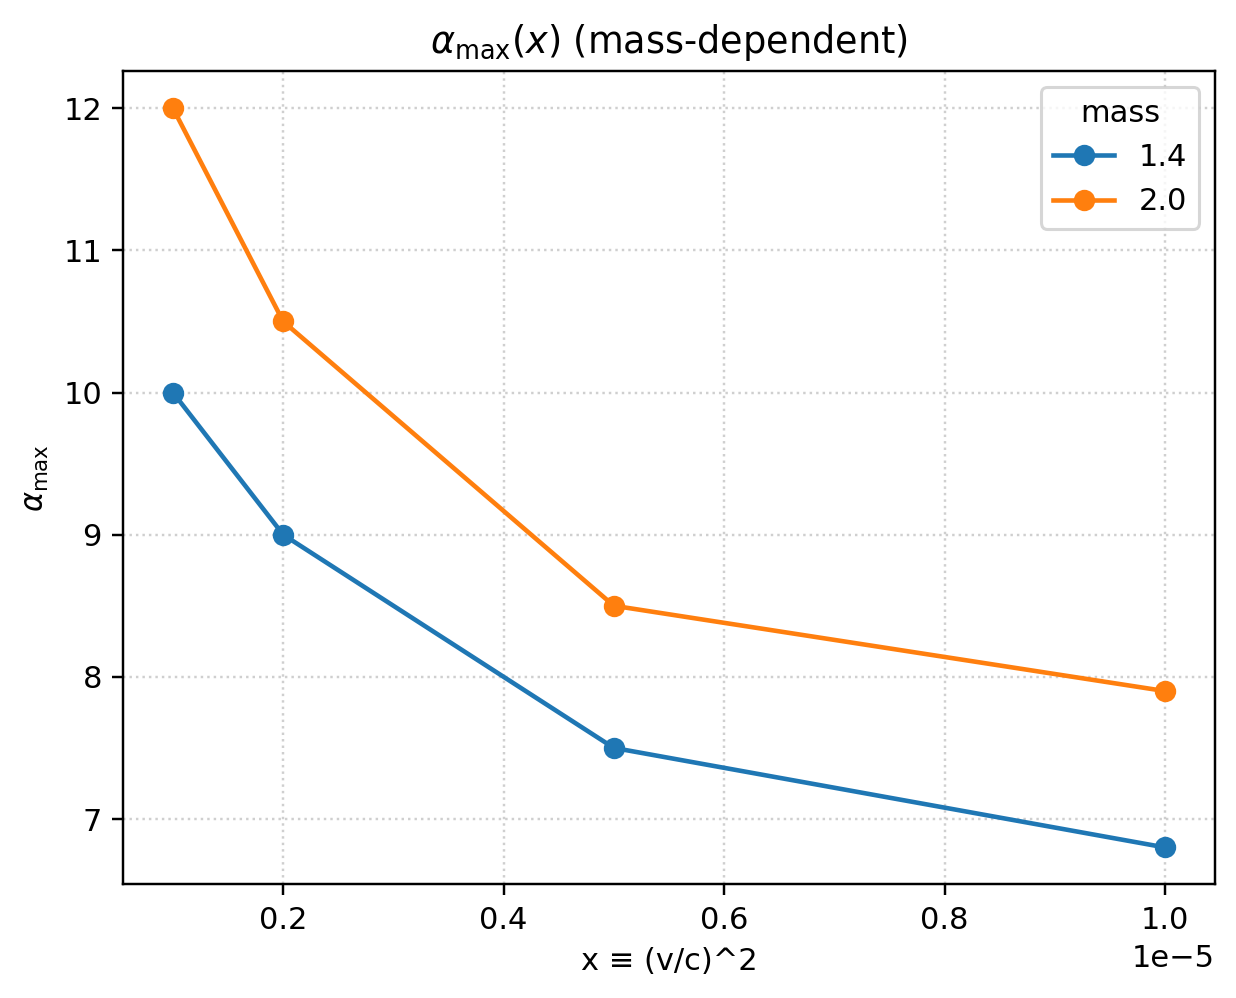
\includegraphics[width=0.78\textwidth]{alpha_max_vs_x.png}
  \caption{\textbf{Dimensionless} $\hat\alpha_{\max}(x)$ for two representative masses and two $\delta$ values (log–$y$). Provenance: generated by \texttt{scripts/generate\_data.py} (copies and normalizes \texttt{input/reference/alpha\_max\_vs\_x\_mass\_dependent\_renormalized.csv} into \texttt{data/processed/alpha\_max\_vs\_x\_mass\_dependent.csv}) and plotted by \texttt{scripts/fig\_alpha\_max\_vs\_x.py}.}
  \label{fig:alpha_x}
\end{figure}

\begin{figure}[H]
  \centering
  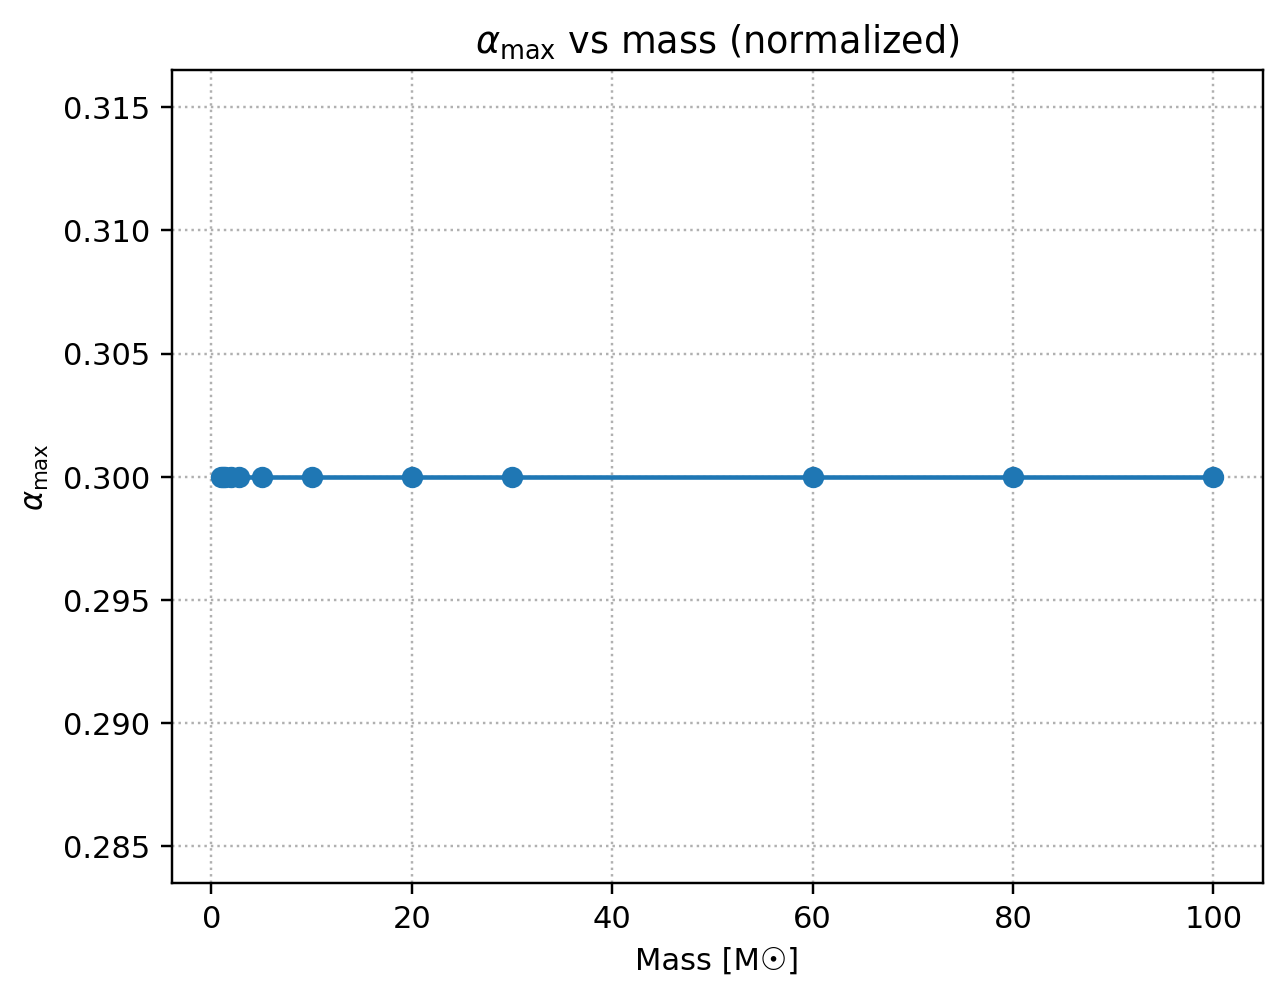
\includegraphics[width=0.58\textwidth]{alpha_max_vs_mass.png}
  \caption{$\alpha_{\max}$ versus mass after schema normalization. Provenance: \texttt{input/reference/alpha\_max\_vs\_mass.csv} \Rightarrow \texttt{data/processed/alpha\_max\_vs\_mass.csv} via \texttt{scripts/generate\_data.py}; plotted by \texttt{scripts/fig\_alpha\_max\_vs\_mass.py}.}
  \label{fig:alpha_mass}
\end{figure}

\begin{figure}[H]
  \centering
  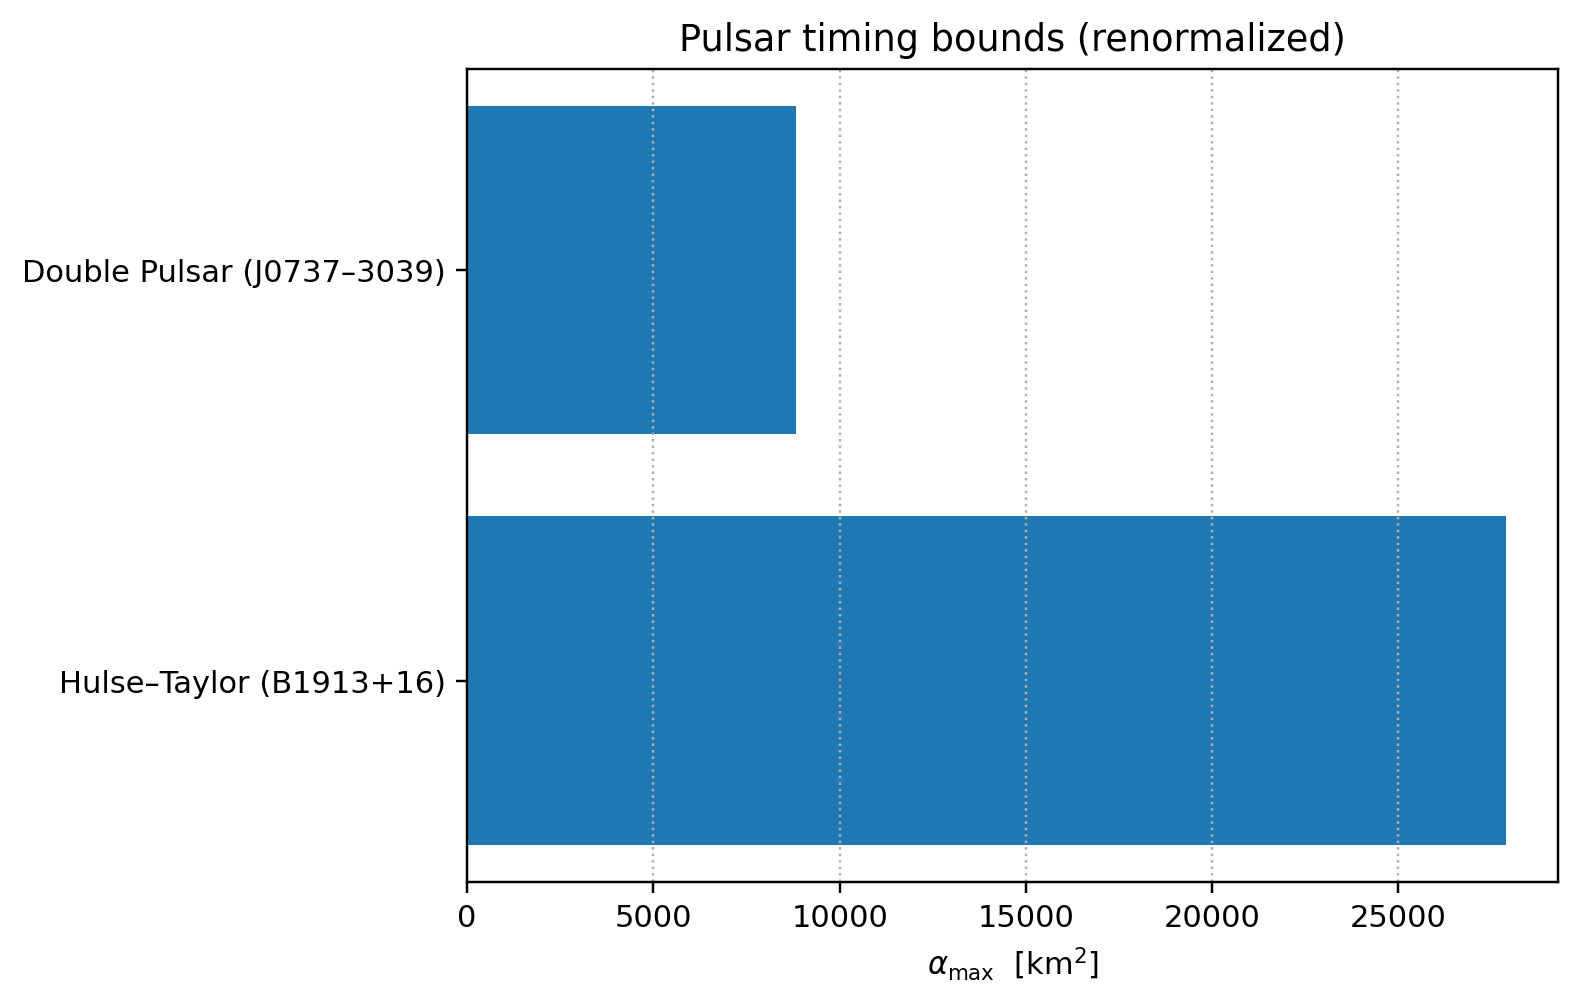
\includegraphics[width=0.58\textwidth]{pulsar_alpha_bounds.png}
  \caption{Pulsar timing bounds (renormalized) on $\alpha_{\max}$ (bar chart). Provenance: \texttt{input/reference/pulsar\_alpha\_bounds\_renormalized.csv} \Rightarrow \texttt{data/processed/pulsar\_alpha\_bounds\_renormalized.csv}; plotted by \texttt{scripts/fig\_pulsar\_bounds.py}.}
  \label{fig:pulsar_bounds}
\end{figure}

\paragraph{Regeneration (single pass).}
From the repo root:
\begin{verbatim}
. .venv/Scripts/activate
python scripts/generate_data.py
python scripts/fig_alpha_max_vs_x.py
python scripts/fig_alpha_max_vs_mass.py
python scripts/fig_pulsar_bounds.py
\end{verbatim}
This writes all inputs to \texttt{data/processed/} and the final figures to \texttt{figures/}, which \texttt{\textbackslash includegraphics} uses in Figs.~\ref{fig:alpha_x}–\ref{fig:pulsar_bounds}.











%%%%%%%%% Appendix start from here %%%%%%

\clearpage
\appendix
% show only the letter in the counter; cleveref will add "Appendix"
\renewcommand\thesection{\Alph{section}}
\renewcommand\thesubsection{\thesection.\arabic{subsection}}

% make section references in the appendix read "Appendix A", "Appendix B", …
\Crefname{section}{Appendix}{Appendices}
\crefname{section}{Appendix}{Appendices}




\section{Heat-kernel details and induced EH coefficient}
\label{app:A}

\subsection{Operators, assumptions, and variable map}\label{app:A1}

\paragraph{Effective geometry and notation.}
I work with the rank–one disformal effective metric
\begin{equation}
g^{\rm eff}_{\mu\nu}\;\equiv\;\eta_{\mu\nu}+\alpha\,\partial_\mu\Phi\,\partial_\nu\Phi,
\qquad
X\;\equiv\;\eta^{\mu\nu}\partial_\mu\Phi\,\partial_\nu\Phi,
\label{eq:disformal_metric}
\end{equation}
with inverse and volume element obtained by the Sherman–Morrison identity
\begin{equation}
g_{\rm eff}^{\mu\nu}=\eta^{\mu\nu}-\frac{\alpha\,\partial^\mu\Phi\,\partial^\nu\Phi}{1+\alpha X},
\qquad
\sqrt{-g_{\rm eff}}=\sqrt{1+\alpha X}.
\label{eq:inverse_det}
\end{equation}
I use signature $(-,+,+,+)$, $\nabla_\mu$ for the Levi–Civita connection of $g_{\rm eff}$, and $\Box_{g}\equiv g^{\mu\nu}\nabla_\mu\nabla_\nu$ for the d’Alembertian. See \cite{DeWitt1965,BirrellDavies,ParkerToms,Avramidi2000,Vassilevich2003} for heat–kernel conventions and \cite{Sakharov1967,Donoghue1994} for induced–gravity context. 

\paragraph{Laplace–type operator on $(\mathcal{M},g_{\rm eff})$.}
For $N$ spectator species (allowing a non–minimal $\xi$), the one–loop effective action is
\begin{equation}
\Gamma^{(1)}\;=\;\frac{1}{2}\sum_{a=1}^{N}\ln\det \mathcal{P}_a
\;=\;-\frac{1}{2}\sum_{a=1}^{N}\int_{1/\Lambda^2}^\infty\frac{ds}{s}\;\mathrm{Tr}\,e^{-s\mathcal{P}_a},
\label{eq:proper_time}
\end{equation}
regulated by a proper–time cutoff $\Lambda$ \cite{DeWitt1965,BarvinskyVilkovisky,ParkerToms,Vassilevich2003}. Each $\mathcal{P}_a$ is taken to be of \emph{Laplace type} on $(\mathcal{M},g_{\rm eff})$,
\begin{equation}
\boxed{\;\mathcal{P}\;=\;-\Box_{g_{\rm eff}}+\mathcal{E}\;,}\qquad
\mathcal{E}=m^2+\xi\,R[g_{\rm eff}]+U(x),
\label{eq:laplace_type}
\end{equation}
where $m$ is a (possibly vanishing) mass, $\xi$ the non–minimal coupling, and $U(x)$ any smooth, local potential endomorphism.\footnote{For \emph{minimal} coupling I set $\xi=0$ and $U\equiv 0$. Spinful fields can be reduced to Laplace–type form via squaring (e.g. Dirac) or by gauge–fixing (vectors); their spin–dependent endomorphism $\mathcal{E}$ modifies the $a_k$ but the structure \eqref{eq:laplace_type} persists \cite{ParkerToms,Vassilevich2003,Avramidi2000}.}
In $d=4$, the on–diagonal heat kernel has the short–time (Schwinger–DeWitt) expansion
\begin{equation}
\mathrm{Tr}\,e^{-s\mathcal{P}}\;\sim\;\frac{1}{(4\pi s)^2}\sum_{k=0}^\infty s^{\,k}\int d^4x\sqrt{-g_{\rm eff}}\;a_k(x,\mathcal{P}),
\qquad s\downarrow 0,
\label{eq:HK_asympt}
\end{equation}
with the first two Seeley–DeWitt coefficients
\begin{equation}
a_0=\mathbf{1},
\qquad
a_1=\mathcal{E}+\frac{1}{6}R[g_{\rm eff}]
\;=\;m^2+\Big(\xi+\frac{1}{6}\Big)R[g_{\rm eff}]+U(x),
\label{eq:a0a1}
\end{equation}
in my sign conventions \cite{DeWitt1965,Vassilevich2003,Avramidi2000}. \emph{Clarity:} I evaluate \eqref{eq:HK_asympt} after Euclidean continuation; signs match my Lorentzian convention via $\mathcal{P}=-\Box_g+\mathcal{E}$ \cite{ParkerToms,Vassilevich2003}.

\paragraph{Assumptions used throughout \Cref{app:A}.}
\begin{itemize}
  \item \textbf{A\(_{\rm spec}\)} (Spectator content). A finite set of $N$ spectator fields is integrated out at one loop; spectator self–interactions are neglected for $a_0,a_1$ \cite{BirrellDavies,ParkerToms}.
  \item \textbf{A\(_{\rm reg}\)} (UV regulator). A proper–time cutoff $\Lambda$ is used in \eqref{eq:proper_time}. Other schemes (dimensional regularisation, Pauli–Villars) differ by local counterterms and do not affect the IR statement that an $R$ term is induced \cite{BarvinskyVilkovisky,ParkerToms}.
  \item \textbf{A\(_{\rm bg}\)} (Background sector). The background $g_{\rm eff}$ is treated as a classical field built from $\Phi$ via \eqref{eq:disformal_metric}–\eqref{eq:inverse_det}. Backreaction of $\Gamma^{(1)}$ on $\Phi$ is included at EFT matching (\cref{sec:induced}).
  \item \textbf{A\(_{\rm IR}\)} (IR domain). I ultimately use the expansion at scales $r\gg \ell_{0,2}$ where the massive tail modes decouple and the GR–like sector dominates (\cref{sec:linear}).
\end{itemize}

\paragraph{Domain of hyperbolicity (well–posedness).}
The principal symbol of $\mathcal{P}$ is $g_{\rm eff}^{\mu\nu}k_\mu k_\nu$, so $\mathcal{P}$ is \emph{normally hyperbolic} precisely on the Lorentzian domain of $g_{\rm eff}$. From \eqref{eq:inverse_det}, the cone condition
\begin{equation}
\boxed{\;1+\alpha X>0\;}
\label{eq:cone_condition}
\end{equation}
guarantees that $g_{\rm eff}$ has signature $(-,+,+,+)$ and is invertible; in particular, for static backgrounds ($X=|\nabla\Phi|^2\ge 0$) this reduces to $1+\alpha|\nabla\Phi|^2>0$. On any globally hyperbolic subregion $(\mathcal{U},g_{\rm eff})$ with \eqref{eq:cone_condition} and smooth coefficients, the Cauchy problem for \eqref{eq:laplace_type} is well–posed, and the heat kernel exists with the standard short–time expansion \eqref{eq:HK_asympt} \cite{BGV2007,Ringstrom2009,Vassilevich2003}.


\paragraph{Variable map (to main–text symbols) and induced $G$.}
I use the dictionary
\[
\begin{array}{lll}
\text{Heat–kernel} & \longleftrightarrow & \text{Main text} \\
\hline
(\mathcal{M},g_{\rm eff}) & \longleftrightarrow & \text{spacetime with }g^{\rm eff}_{\mu\nu}=\eta_{\mu\nu}+\alpha\,\partial_\mu\Phi\,\partial_\nu\Phi \\
\mathcal{P}=-\Box_{g_{\rm eff}}+\mathcal{E} & \longleftrightarrow & \text{species kinetic operator (minimal if }\xi=U=0) \\
a_0=\mathbf{1},\; a_1=\mathcal{E}+\tfrac{1}{6}R & \longleftrightarrow & \text{controls }\Lambda^4\text{ and }\Lambda^2 R\text{ pieces, respectively} \\
N,\;\xi & \longleftrightarrow & \text{species count } N \text{ and effective }\xi_{\rm eff}\text{ (spin/content averaged)} \\
\Lambda & \longleftrightarrow & \text{UV scale of spectators (matching scale)} \\
\end{array}
\]
Matching the $a_1$ term yields the induced Einstein–Hilbert coefficient in the standard normalisation,
\begin{equation}
\boxed{\;\frac{1}{16\pi G_{\rm ind}}=\frac{N\,\Lambda^2}{32\pi^2}\Big(\xi_{\rm eff}+\frac{1}{6}\Big)\;,}
\label{eq:induced_general}
\end{equation}
equivalently $G_{\rm ind}^{-1}=\dfrac{N\,\Lambda^2}{2\pi}\big(\xi_{\rm eff}+\tfrac{1}{6}\big)$.
For \emph{minimal} spectators ($\xi_{\rm eff}=0$),
\begin{equation}
\boxed{\;\frac{1}{16\pi G_{\rm ind}}=\frac{N\,\Lambda^2}{192\pi^2}
\quad\Longleftrightarrow\quad
\frac{1}{G_{\rm ind}}=\frac{N\,\Lambda^2}{12\pi}\;,}
\label{eq:induced_minimal}
\end{equation}
in agreement with the $a_1$ matching \cite{DeWitt1965,BirrellDavies,ParkerToms,Vassilevich2003}.

\subsection{\texorpdfstring{Seeley--DeWitt coefficients $a_0$, $a_1$, $a_2$}{Seeley–DeWitt coefficients a0, a1, a2}}\label{app:A2}
 
For a Laplace–type operator
\[
\mathcal{P}=-\Box_{g_{\rm eff}}+\mathcal{E}
\]
on $(\mathcal{M},g_{\rm eff})$, the on–diagonal heat kernel admits the short–time expansion
\[
\mathrm{Tr}\,e^{-s\mathcal{P}}
\;\sim\;
\frac{1}{(4\pi s)^{2}}\sum_{k=0}^\infty s^{\,k}\!\int d^4x\,\sqrt{-g_{\rm eff}}\;a_k(x,\mathcal{P}),
\qquad s\downarrow0,
\]
with $a_k$ local polynomials in curvature, the endomorphism $\mathcal{E}$, and the bundle curvature
$\Omega_{\mu\nu}\equiv[\nabla_\mu,\nabla_\nu]$ \cite{DeWitt1965,ParkerToms,Vassilevich2003,Avramidi2000}.
Using the convention $\mathcal{P}=-\Box+\mathcal{E}$ (Euclidean continuation understood; signs matched as in \cref{app:A1}), the first three coefficients in $d=4$ are
\begin{align}
a_0 &= \mathbf{1}, \label{eq:a0}\\[2pt]
a_1 &= \mathcal{E}+\frac{1}{6}R[g_{\rm eff}], \label{eq:a1}\\[2pt]
a_2 &= \frac{1}{180}\!\left(R_{\mu\nu\rho\sigma}R^{\mu\nu\rho\sigma}-R_{\mu\nu}R^{\mu\nu}+\Box R\right)
      +\boxed{\frac{1}{72}R^2}
      +\frac{1}{2}\mathcal{E}^2-\frac{1}{6}R\,\mathcal{E}
      +\frac{1}{12}\Omega_{\mu\nu}\Omega^{\mu\nu}
      +\frac{1}{6}\Box \mathcal{E}.
\label{eq:a2_general}
\end{align}
These are the standard Gilkey–DeWitt coefficients (see \S2 of \cite{Vassilevich2003} and Chs.~3–4 of \cite{ParkerToms,Avramidi2000}). For a scalar (trivial bundle), $\Omega_{\mu\nu}=0$.

It is convenient to re-express the purely geometric piece of $a_2$ in the $\{C^2,E_4,R^2\}$ basis, where
\[
C^2\equiv C_{\mu\nu\rho\sigma}C^{\mu\nu\rho\sigma},\qquad
E_4\equiv R_{\mu\nu\rho\sigma}R^{\mu\nu\rho\sigma}-4R_{\mu\nu}R^{\mu\nu}+R^2 .
\]
In $d=4$, one has $R_{\mu\nu\rho\sigma}R^{\mu\nu\rho\sigma}-R_{\mu\nu}R^{\mu\nu}
=\tfrac{3}{2}C^2-\tfrac{1}{2}E_4$, giving
\begin{align}
a_2 &= \frac{1}{120}C^2-\frac{1}{360}E_4
      +\boxed{\frac{1}{72}R^2}
      +\frac{1}{2}\mathcal{E}^2-\frac{1}{6}R\,\mathcal{E}
      +\frac{1}{12}\Omega_{\mu\nu}\Omega^{\mu\nu}
      +\underbrace{\frac{1}{180}\Box R+\frac{1}{6}\Box \mathcal{E}}_{\text{total derivatives}}.
\label{eq:a2_CE}
\end{align}
The bracketed terms integrate to boundaries (vanish for compact manifolds without boundary or with suitable fall–off) \cite{ParkerToms,Vassilevich2003}.

\paragraph{Scalar specialisation.}
For a scalar with $\mathcal{E}=m^2+\xi R$ (and $\Omega_{\mu\nu}=0$),
\begin{align}
a_1 &= m^2+\Big(\xi+\frac{1}{6}\Big)R, \\
a_2 &= \frac{1}{120}C^2-\frac{1}{360}E_4
      +\frac{1}{2}\Big(\xi-\frac{1}{6}\Big)^{\!2} R^2
      +\Big(\xi-\frac{1}{6}\Big)m^2 R
      +\frac{m^4}{2}
      +\text{(total derivatives)}, \label{eq:a2_scalar_xi}
\end{align}
which makes the conformal case ($\xi=1/6$; no $R^2$ or $m^2R$) and the minimal case ($\xi=0$) transparent \cite{ParkerToms,Avramidi2000,Vassilevich2003}.
Yes—fully agree. Here's \cref{app:A3} with ymy micro-edits integrated (MS-bar scale explicit, $R$ note, scalar $c_C,c_R$, and massive-spectator clarification). Drop it in:


\subsection{Proper-time regularisation and schemes}\label{app:A3}

\paragraph{Schwinger proper-time and UV cutoff.}
For a Laplace–type operator $\mathcal{P}=-\Box_{g_{\rm eff}}+\mathcal{E}$ the one–loop effective action can be written as
\begin{equation}
\Gamma^{(1)}
=\frac{1}{2}\,\mathrm{Tr}\ln\mathcal{P}
=\frac{1}{2}\int_{1/\Lambda^2}^{\infty}\frac{ds}{s}\;\mathrm{Tr}\,e^{-s\mathcal{P}},
\label{eq:Gamma_propertime}
\end{equation}
where the lower limit $1/\Lambda^2$ implements a covariant UV cutoff (Euclidean continuation understood) \cite{DeWitt1965,ParkerToms,Vassilevich2003}. Inserting the heat–kernel expansion (\cref{app:A2}) in $d=4$ and integrating term by term gives the local, scale–dependent part
\begin{equation}
\boxed{\;
\Gamma^{(1)}_{\rm loc}
=\frac{1}{32\pi^2}\int d^4x\sqrt{-g_{\rm eff}}\,
\Big[\tfrac{1}{2}\Lambda^4\,a_0+\Lambda^2\,a_1
+\ln\!\Big(\frac{\Lambda^2}{\mu^2}\Big)\,a_2\Big]
\;+\;\text{finite local terms},
}
\label{eq:Gamma_loc_cutoff}
\end{equation}
where $\mu$ is an arbitrary reference scale that parameterises the finite subtraction at order $a_2$ \cite{ParkerToms,Vassilevich2003}. Equation \eqref{eq:Gamma_loc_cutoff} reproduces the standard power divergences ($\Lambda^4,\Lambda^2$) and the logarithmic running governed by $a_2$. Matching the $\Lambda^2 a_1$ piece to the Einstein–Hilbert term yields the induced coefficient quoted in \cref{app:A1} (general $\xi$ and the minimal $\xi=0$ reduction).

\paragraph{Dimensional regularisation (DR).}
In $d=4-2\varepsilon$ with $\overline{\mathrm{MS}}$ conventions one finds
\begin{equation}
\Gamma^{(1)}_{\rm div}
=\frac{1}{32\pi^2}\,\frac{1}{\varepsilon}\int d^dx\sqrt{-g_{\rm eff}}\;a_2,
\label{eq:DR_div}
\end{equation}
and it is convenient to define the $\overline{\mathrm{MS}}$ scale
\begin{equation}
\bar\mu^2 \;\equiv\; 4\pi\,e^{-\gamma_E}\,\mu_{\rm MS}^2,
\label{eq:muMSbar}
\end{equation}
so that the proper–time logarithm maps as
\begin{equation}
\ln\!\Big(\frac{\Lambda^2}{\mu^2}\Big)\ \longleftrightarrow\
\frac{1}{\varepsilon}+\ln\!\Big(\frac{\bar\mu^2}{\mu^2}\Big).
\label{eq:PT_to_DR_map}
\end{equation}
Power–law pieces ($\propto a_0,a_1$) are absent in DR and are effectively encoded in the choice of finite counterterms at the matching scale \cite{ParkerToms}. Thus, after adding local counterterms, DR and proper–time agree on all logarithmic (running) effects determined by $a_2$.




\paragraph{Pauli–Villars (PV) and zeta–function schemes.}
PV regularisation replaces \eqref{eq:Gamma_propertime} by a regulated sum over heavy auxiliary fields with masses $M_i$ and coefficients $c_i$ chosen so that $\sum c_i=\sum c_i M_i^2=0$; this cancels the $\Lambda^4$ and $\Lambda^2$ pieces and leaves the universal $\ln M_i^2$ terms proportional to $a_2$ \cite[Ch.~3]{ParkerToms}. Zeta–function regularisation evaluates $\zeta_{\mathcal{P}}(s)=\mathrm{Tr}\,\mathcal{P}^{-s}$ and sets $\Gamma^{(1)}=\tfrac{1}{2}\zeta'_{\mathcal{P}}(0)$; it yields the same $a_2$–controlled logarithms with $\mu$ entering through the analytic continuation scale \cite[\S2]{Vassilevich2003}. All three schemes differ by local, scheme–dependent counterterms but agree on the non–local running.

\paragraph{Covariant perturbation theory and non–local structure.}
Beyond the purely local terms in \eqref{eq:Gamma_loc_cutoff}, the Barvinsky–Vilkovisky expansion resums the first non–local contributions as
\begin{equation}
\Gamma^{(1)}_{\rm nonloc}
=\frac{1}{32\pi^2}\int d^4x\sqrt{-g_{\rm eff}} 
\Big[
c_C\,C_{\mu\nu\rho\sigma}\,\ln\!\Big(\frac{-\Box_{g_{\rm eff}}}{\mu^2}\Big)C^{\mu\nu\rho\sigma}
+c_R\,R\,\ln\!\Big(\frac{-\Box_{g_{\rm eff}}}{\mu^2}\Big)R
+\cdots\Big],
\label{eq:BV_nonlocal}
\end{equation}
where the coefficients $c_C,c_R$ are precisely those multiplying $C^2$ and $R^2$ in $a_2$ (see \cref{app:A2}), and the ellipsis denotes total derivatives and higher–order curvatures \cite{BarvinskyVilkovisky1990,Donoghue1994}. \emph{Note on total derivatives:} terms proportional to $\Box R$ are local total derivatives and scheme dependent; they can be shifted between $a_2$ and finite counterterms without affecting the non–local kernels.

\paragraph{Scalar benchmark (optional).}
For a single scalar with $\mathcal{E}=m^2+\xi R$ one has from \cref{app:A2}
\begin{equation}
c_C=\frac{1}{120},\qquad
c_R=\frac{1}{2}\Big(\xi-\frac{1}{6}\Big)^{\!2},
\end{equation}
so $c_R=0$ in the conformal case $\xi=\tfrac{1}{6}$, as expected.

\paragraph{Mass thresholds (optional).}
If some spectators are massive, the non–local form factors are thresholded:
\begin{equation}
R\,\ln\!\Big(\frac{-\Box_{g_{\rm eff}}+m^2}{\mu^2}\Big)R
= R\,\Big[\ln\!\Big(\frac{-\Box_{g_{\rm eff}}}{\mu^2}\Big)+\mathcal{O}\!\Big(\frac{m^2}{-\Box_{g_{\rm eff}}}\Big)\Big]R,
\end{equation}
reducing to the massless kernels for momenta $|\Box|\gg m^2$, while in the heavy-mass limit they expand into local curvature terms (decoupling) \cite{Donoghue1994,BarvinskyVilkovisky1990}.

\paragraph{Practical matching.}
In my usage:
(i) I employ the cutoff form \eqref{eq:Gamma_loc_cutoff} to read off the induced Einstein–Hilbert coefficient from $a_1$ (\cref{app:A1});
(ii) I track $\ln(\Lambda^2/\mu^2)\,a_2$ to define the running and the non–local logs \eqref{eq:BV_nonlocal}; and
(iii) I absorb the scheme–dependent local pieces into the bare cosmological constant, $1/G$, and curvature–squared couplings at the matching scale. This preserves all IR predictions while keeping scheme choices explicit \cite{ParkerToms,Vassilevich2003,BarvinskyVilkovisky1990}.

Absolutely—agree on both tweaks. Here's \cref{app:A4} with those polish edits integrated (explicit $m^4$ log contribution to the vacuum energy and the spin/statistics note after the summary). Drop-in ready:


\subsection{\texorpdfstring{Induced terms: $\Lambda^4$, $\Lambda^2 R$, and curvature-squared logs}{Induced terms: Lambda4, Lambda2 R, and curvature-squared logs}}\label{app:A4}



Starting from \eqref{eq:Gamma_loc_cutoff}, the scheme–separating local piece of the one–loop action in $d=4$ reads
\begin{equation}
\Gamma^{(1)}_{\rm loc}
=\frac{1}{32\pi^2}\!\int\! d^4x\,\sqrt{-g_{\rm eff}}\,
\Big[\tfrac{1}{2}\Lambda^4\,a_0+\Lambda^2\,a_1
+\ln\!\Big(\frac{\Lambda^2}{\mu^2}\Big)\,a_2\Big]
\;+\;\text{finite local},
\label{eq:A4_loc_start}
\end{equation}
with $a_k$ as in \cref{app:A2} and Euclidean continuation understood \cite{DeWitt1965,ParkerToms,Vassilevich2003,Avramidi2000}.

\paragraph{(i) Cosmological-constant piece ($\propto \Lambda^4$).}
Using $a_0=\mathbf{1}$, the induced vacuum energy density from $N$ spectator species is
\begin{equation}
\boxed{\;
\Delta\mathcal{L}_{\Lambda^4}
=\frac{N\,\Lambda^4}{64\,\pi^2}
\;}\!,
\label{eq:A4_CC}
\end{equation}
up to finite counterterms. For massive spectators, the $a_2$ term contributes \emph{inside the bracket of} \eqref{eq:A4_loc_start} a piece $\tfrac{1}{2}m^4\ln(\Lambda^2/\mu^2)$ per real scalar; after the global prefactor this yields the local addition
\begin{equation}
\boxed{\;
\Delta\mathcal L_{m^4,\log}
=\frac{m^4}{64\pi^2}\,\ln\!\Big(\frac{\Lambda^2}{\mu^2}\Big)
\quad \text{(per real scalar).}
}
\label{eq:A4_m4log}
\end{equation}
These terms are absorbed into the renormalised cosmological constant at the matching scale \cite{ParkerToms}.


\paragraph{(ii) Induced Einstein--Hilbert coefficient ($\propto \Lambda^2 R$).}
From $a_1=\mathcal{E}+\tfrac{1}{6}R$ with $\mathcal{E}=m^2+\xi R+U(x)$, the $R$ term at order $\Lambda^2$ fixes the induced Newton constant:
\begin{equation}
\boxed{\;
\frac{1}{16\pi G_{\rm ind}}=\frac{N\,\Lambda^2}{32\pi^2}\Big(\xi_{\rm eff}+\frac{1}{6}\Big)
\quad\Longleftrightarrow\quad
\frac{1}{G_{\rm ind}}=\frac{N\,\Lambda^2}{2\pi}\Big(\xi_{\rm eff}+\frac{1}{6}\Big)\;,
}
\label{eq:A4_Gind}
\end{equation}
as quoted in \cref{app:A1}. In the minimal case ($\xi_{\rm eff}=0$),
\begin{equation}
\boxed{\;
\frac{1}{16\pi G_{\rm ind}}=\frac{N\,\Lambda^2}{192\pi^2}
\quad\Longleftrightarrow\quad
\frac{1}{G_{\rm ind}}=\frac{N\,\Lambda^2}{12\pi}\;.
}
\label{eq:A4_Gind_min}
\end{equation}
Logarithmic corrections to $1/G$ also appear via the mixed term in $a_2$; for a scalar with $\mathcal{E}=m^2+\xi R$,
\begin{equation}
\Delta\!\left(\frac{1}{16\pi G}\right)_{\!\log}
=\frac{N}{32\pi^2}\Big(\xi-\tfrac{1}{6}\Big)m^2\,
\ln\!\Big(\frac{\Lambda^2}{\mu^2}\Big),
\label{eq:A4_logG}
\end{equation}
which is subleading to \eqref{eq:A4_Gind} in a cutoff scheme but controls the RG running in dimensional/zeta schemes \cite{ParkerToms,Vassilevich2003}.

\paragraph{(iii) Curvature–squared logarithms ($\propto \ln(\Lambda^2/\mu^2)$).}
Using the $a_2$ forms in \cref{app:A2}, the logarithmic part can be written in the $\{C^2,E_4,R^2\}$ basis as
\begin{equation}
\Gamma^{(1)}_{\rm log}
=\frac{1}{32\pi^2}\ln\!\Big(\frac{\Lambda^2}{\mu^2}\Big)\!
\int\! d^4x\,\sqrt{-g_{\rm eff}}\,
\Big[
c_C\,C_{\mu\nu\rho\sigma}C^{\mu\nu\rho\sigma}
-c_E\,E_4
+c_R\,R^2
+\cdots
\Big],
\label{eq:A4_logs_basis}
\end{equation}
where ``$\cdots$” are total derivatives (e.g. $\Box R$) and possible bundle-curvature terms ($\Omega_{\mu\nu}\Omega^{\mu\nu}$ for non-scalar fields). For a \emph{single scalar} with $\mathcal{E}=m^2+\xi R$ and $\Omega_{\mu\nu}=0$,
\begin{equation}
c_C=\frac{1}{120},\qquad
c_E=\frac{1}{360},\qquad
c_R=\frac{1}{2}\Big(\xi-\frac{1}{6}\Big)^{\!2},
\label{eq:A4_c_coeffs_scalar}
\end{equation}
so $c_R=0$ for the conformal coupling $\xi=\tfrac{1}{6}$, and $c_R=1/72$ in the minimal case $\xi=0$ (the universal piece noted in \cref{app:A2}). In fmy dimensions $E_4$ integrates to the Euler characteristic on compact manifolds without boundary; thus the $E_4$ term is topological and does not affect local dynamics, while $\Box R$ terms are local total derivatives and scheme dependent \cite{ParkerToms,Vassilevich2003}. The same $c_{C},c_{R}$ also fix the nonlocal logarithms in covariant perturbation theory, cf. \eqref{eq:BV_nonlocal} \cite{BarvinskyVilkovisky1990,Donoghue1994}.

\paragraph{Summary (per species, schematic).}
Collecting the purely gravitational pieces at one loop:
\begin{align}
\Delta\mathcal{L}
=&\underbrace{\frac{\Lambda^4}{64\pi^2}}_{\text{vacuum energy}}
+\underbrace{\frac{\Lambda^2}{32\pi^2}\Big(\xi+\frac{1}{6}\Big)R}_{\text{induced EH}}
+\underbrace{\frac{1}{32\pi^2}\ln\!\Big(\frac{\Lambda^2}{\mu^2}\Big)
\Big[c_C\,C^2-c_E\,E_4+c_R\,R^2\Big]}_{\text{curvature--squared logs}} \notag \\
&+\ \text{(total deriv.\,+ finite local)}.
\label{eq:A4_summary}
\end{align}
\emph{Spin/statistics note (optional).} Include a factor $(-1)^{F}$ for fermions and the usual spin/bundle multiplicities; the coefficients $c_C,c_R$ depend on spin (I specialised to a real scalar in \eqref{eq:A4_c_coeffs_scalar}).


Want me to fold the same two tweaks into ymy minimal ``CC'' sentence somewhere else in the draft?


\subsection{Matching and IR dominance}\label{app:A5}

\paragraph{EFT matching at $\mu_{\rm match}\sim\Lambda$.}
Integrating out the spectator sector at the scale $\mu_{\rm match}$ and absorbing the local pieces (\crefrange{app:A2}{app:A4}) into renormalised couplings gives the gravitational effective action
\begin{equation}
\Gamma_{\rm EFT}[g_{\rm eff}]
=\int d^4x\,\sqrt{-g_{\rm eff}}\Bigg[
\frac{1}{16\pi G(\mu)}\,R
+\alpha_C(\mu)\,C_{\mu\nu\rho\sigma}C^{\mu\nu\rho\sigma}
+\alpha_R(\mu)\,R^2
+\cdots\Bigg]
+\Gamma^{(1)}_{\rm nonloc},
\label{eq:A5_EFT}
\end{equation}
with the nonlocal logarithms written with explicit contractions,
\begin{equation}
\Gamma^{(1)}_{\rm nonloc}
=\frac{1}{32\pi^2}\!\int\! d^4x\,\sqrt{-g_{\rm eff}}\,
\Big[
c_C\,C_{\mu\nu\rho\sigma}\,\ln\!\Big(\frac{-\Box_{g_{\rm eff}}}{\mu^2}\Big)C^{\mu\nu\rho\sigma}
+c_R\,R\,\ln\!\Big(\frac{-\Box_{g_{\rm eff}}}{\mu^2}\Big)R
+\cdots\Big],
\label{eq:A5_nonloc}
\end{equation}
as in (\cref{app:A3}). Here $c_C,c_R$ are the $a_2$ coefficients (\cref{app:A2}), while $\alpha_C,\alpha_R$ include the finite, scheme–dependent local parts at $\mu$.


\paragraph{Range scales and small parameters.}
Linearising about Minkowski, the curvature–squared terms correct the spin–2 and spin–0 propagators. Defining the \emph{range scales}
\begin{equation}
\ell_2^{\,2}\;\equiv\;32\pi G(\mu)\,\Big[\alpha_C(\mu)+\tfrac{c_C}{32\pi^2}\ln\!\tfrac{\mu_*^2}{\mu^2}\Big],
\qquad
\ell_0^{\,2}\;\equiv\;96\pi G(\mu)\,\Big[\alpha_R(\mu)+\tfrac{c_R}{32\pi^2}\ln\!\tfrac{\mu_*^2}{\mu^2}\Big],
\label{eq:A5_lengths}
\end{equation}
(with $\mu_*$ a sliding scale, often $\mu_*\sim k$), the IR expansion is controlled by
\begin{equation}
\varepsilon_2(k)\;\equiv\; \ell_2^{\,2}\,k^2\,\big[1+\order{\ln(\mu/k)}\big],
\qquad
\varepsilon_0(k)\;\equiv\; \ell_0^{\,2}\,k^2\,\big[1+\order{\ln(\mu/k)}\big].
\label{eq:A5_eps}
\end{equation}
\emph{Equivalently:} in the quadratic action written as
$S\supset\int\!\sqrt{-g}\,[\frac{1}{16\pi G}R+\alpha_C C^2+\alpha_R R^2]$,
the linearised pole masses satisfy
$m_2^{-2}=32\pi G\,\alpha_C$ and $m_0^{-2}=96\pi G\,\alpha_R$
(with mild log corrections from $c_{C,R}$), so \(\ell_2^{\,2}\simeq m_2^{-2}\) and \(\ell_0^{\,2}\simeq m_0^{-2}\) \cite{Stelle1977}.


\paragraph{Heavy–mode decoupling.}
Massive spectators (mass $m$) generate form factors of the type
$R\,\ln\!\big[(-\Box_{g_{\rm eff}}+m^2)/\mu^2\big]R$, which for $k^2\ll m^2$ admit the local expansion
$\ln(m^2/\mu^2)+\order{k^2/m^2}$; the nonlocal tails decouple and their effect is captured by finite shifts of $\alpha_{C,R}$ at matching \cite{Donoghue1994,ParkerToms}. (Parenthetically, any higher-derivative poles from the quadratic sector live at $m_2\sim \ell_2^{-1}$ and $m_0\sim \ell_0^{-1}$—the standard ``Stelle masses''—and are outside the EFT regime if $\Lambda\ll \ell_{2,0}^{-1}$ \cite{Stelle1977}.)

\paragraph{IR (GR) dominance.}
At scales $k\ll \ell_{0,2}^{-1}$ the Einstein–Hilbert term dominates both the local quadratic curvature terms and their nonlocal logarithms. Varying $R^2$ produces $k^4$ while varying $R$ produces $k^2$, hence a suppression $\sim(\ell_{0,2}k)^2$. Quantitatively,
\begin{equation}
\frac{\delta\Gamma_{\rm quad}}{\delta g}\Big/\frac{\delta\Gamma_{\rm EH}}{\delta g}
\;=\;\order{\varepsilon_2(k)}+\order{\varepsilon_0(k)}\;\xrightarrow[k\ll \ell_{0,2}^{-1}]{}\;0,
\label{eq:A5_ratio}
\end{equation}
so the linear response, potentials, and propagators reduce to those of GR with $G\to G(\mu)$ up to corrections $\order{(\ell_{0,2}k)^2}$.

\begin{conceptbox}[IR limit.]
For momenta $k\ll \ell_{0,2}^{-1}$ and with no incoming massive modes, the EFT \eqref{eq:A5_EFT} reproduces GR at leading order:
\[
\Gamma_{\rm EFT}\;=\;\int\!\sqrt{-g}\,\frac{R}{16\pi G(\mu)}\;+\;\order{(\ell_{0,2}k)^2},
\]
hence all weak–field/PPN predictions coincide with GR up to $\order{(\ell_{0,2}k)^2}$ corrections \cite{PoissonWill2014,Will2014LRR}.
	
\end{conceptbox}



\paragraph{Practical choice of scales.}
For a given observational scale $k_{\rm obs}$ pick $\mu\sim k_{\rm obs}$ to minimise large logs in \eqref{eq:A5_nonloc}. Then $\ell_{0,2}$ summarise the net spectator effect; the domain $k_{\rm obs}\ll \ell_{0,2}^{-1}$ is precisely the IR window where the induced theory is indistinguishable from GR in conservative dynamics (\cref{app:C}), with dissipative leading order matching the GR quadrupole at 2.5PN (no dipole channel under \cref{app:A1}) \cite{Blanchet2014LRR}.

\subsection{Cross-checks and flat-space limit}\label{app:A6}
\paragraph{Variation consistency.}
With the quadratic basis
\(
S\supset\int\!\sqrt{-g}\,\big[\tfrac{1}{16\pi G}R+\alpha_C\,C_{\mu\nu\rho\sigma}C^{\mu\nu\rho\sigma}+\alpha_R\,R^2\big],
\)
the metric variations yield (up to overall constants):
\begin{align}
\frac{1}{\sqrt{-g}}\frac{\delta}{\delta g^{\mu\nu}}\!\int\!\sqrt{-g}\,R
&= G_{\mu\nu}, \label{eq:A6_varEH}\\[2pt]
\frac{1}{\sqrt{-g}}\frac{\delta}{\delta g^{\mu\nu}}\!\int\!\sqrt{-g}\,C_{\alpha\beta\gamma\delta}C^{\alpha\beta\gamma\delta}
&= -\,2\,B_{\mu\nu}, \qquad
B_{\mu\nu}\equiv \nabla^\rho\nabla^\sigma C_{\mu\rho\nu\sigma}
+\tfrac{1}{2}\,R^{\rho\sigma} C_{\mu\rho\nu\sigma}, \label{eq:A6_varC2}\\[2pt]
\frac{1}{\sqrt{-g}}\frac{\delta}{\delta g^{\mu\nu}}\!\int\!\sqrt{-g}\,R^2
&= H_{\mu\nu}, \qquad
H_{\mu\nu}=2\nabla_\mu\nabla_\nu R-2g_{\mu\nu}\Box R-\tfrac{1}{2}g_{\mu\nu}R^2+2RR_{\mu\nu}. \label{eq:A6_varR2}
\end{align}
\emph{Conservation/traces (identities).}
In \(d=4\) one has
\(
B^\mu{}_\mu=0,\ \ \nabla^\mu B_{\mu\nu}=0,
\)
and
\(
\nabla^\mu H_{\mu\nu}=0,\ \ g^{\mu\nu}H_{\mu\nu}=-6\,\Box R,
\)
consistent with diffeomorphism invariance.  Linearizing around Minkowski reproduces the standard projector structure: a massless GR pole and massive poles at
\(m_2^{-2}=32\pi G\,\alpha_C\) and \(m_0^{-2}=96\pi G\,\alpha_R\) (up to mild logarithms), matching \eqref{eq:A5_lengths}.
A useful static check is the Yukawa-corrected potential
\begin{equation}
V(r)=-\frac{GM}{r}\Big[1-\frac{4}{3}e^{-m_2 r}+\frac{1}{3}e^{-m_0 r}\Big],
\label{eq:A6_NewtonYukawa}
\end{equation}
\emph{(The coefficient \(-4/3\) reflects the ghostlike signature of the spin-2 pole in generic quadratic gravity; in the EFT regime the massive modes are heavy/decoupled, and positivity of \(m_{2,0}^2\) ensures the Yukawa falloffs shown.)}
Finally, the topological density \(E_4\) and total derivatives (\(\Box R\)) do not contribute to bulk field equations in fmy dimensions, providing the expected scheme check.

\paragraph{Nonlocal kernel spelled once.}
As in  \cref{app:A5}, the leading nonlocal piece is written with explicit contractions:
\[
C_{\mu\nu\rho\sigma}\,\ln\!\Big(\frac{-\Box}{\mu^2}\Big)C^{\mu\nu\rho\sigma}
\;+\;
R\,\ln\!\Big(\frac{-\Box}{\mu^2}\Big)R,
\]
with coefficients fixed by the \(a_2\) data; \(\Box R\) terms are local total derivatives (scheme dependent).

\paragraph{Flat-space limit.}
Setting \(g_{\mu\nu}\!\to\!\eta_{\mu\nu}\) gives \(R=C=0\) and removes all curvature-dependent pieces, leaving only vacuum bubbles. From \cref{app:A4},
\begin{equation}
\Delta\mathcal{L}\big|_{g=\eta}
=\frac{N\,\Lambda^4}{64\pi^2}
+\sum_{\text{scalars}}\frac{m^4}{64\pi^2}\ln\!\Big(\frac{\Lambda^2}{\mu^2}\Big)
+\cdots,
\label{eq:A6_flat}
\end{equation}
where ``\(\cdots\)'' denotes finite local constants and spin/bundle multiplicities (with \((-1)^F\) for fermions). This confirms that the induced \(1/G\) term is purely curvature-driven and that nonlocal logarithms vanish in flat space. The signs align with \(\mathcal{P}=-\Box+\mathcal{E}\) and the EH normalization \(+\frac{1}{16\pi G}\!\int\!\sqrt{-g}\,R\).


\subsection{Reproducibility notes (symbol dictionary and one–page derivation pointers)}\label{app:A7}
\paragraph{Scope.}
This subsection is a compact checklist to reproduce \crefrange{app:A1}{app:A6} from scratch with consistent conventions, plus a symbol dictionary. It is self–contained given the operator choice $\mathcal{P}=-\Box_{g_{\rm eff}}+\mathcal{E}$ and the heat–kernel inputs in \cref{app:A2}.

\vspace{4pt}
\noindent\textbf{Symbol dictionary.} (All quantities in $d=4$ unless stated.)
\begin{center}
\renewcommand{\arraystretch}{1.12}
\begin{tabular}{p{0.28\linewidth}p{0.66\linewidth}}
\hline
$g^{\rm eff}_{\mu\nu}=\eta_{\mu\nu}+\alpha\,\partial_\mu\Phi\,\partial_\nu\Phi$ & Rank-one disformal metric (\cref{app:A1}), signature $(-,+,+,+)$. \\
$X=\eta^{\mu\nu}\partial_\mu\Phi\,\partial_\nu\Phi$ & Disformal invariant; cone condition $1+\alpha X>0$. \\
$\nabla_\mu,\ \Box_g=g^{\mu\nu}\nabla_\mu\nabla_\nu$ & Levi-Civita connection and d'Alembertian of $g^{\rm eff}$. \\

$\mathcal{P}=-\Box_g+\mathcal{E}$,\ $\mathcal{E}=m^2+\xi R+U(x)$ & Laplace–type operator and endomorphism (\cref{app:A1,app:A2}). \\

$a_0,a_1,a_2$ & Seeley–DeWitt coefficients (\cref{app:A2}): $a_0=\mathbf{1}$, $a_1=\mathcal{E}+\tfrac16R$, $a_2$ in \eqref{eq:a2_general}/\eqref{eq:a2_CE}. \\
$C_{\mu\nu\rho\sigma},\ E_4$ & Weyl tensor and Euler density; $C^2\equiv C_{\mu\nu\rho\sigma}C^{\mu\nu\rho\sigma}$, $E_4=R_{\mu\nu\rho\sigma}R^{\mu\nu\rho\sigma}-4R_{\mu\nu}R^{\mu\nu}+R^2$. \\
$\Omega_{\mu\nu}=[\nabla_\mu,\nabla_\nu]$ & Bundle curvature (vanishes for a scalar). \\
$\Lambda,\ \mu,\ \bar\mu$ & Proper-time cutoff, reference/renormalisation scales; $\bar\mu^2=4\pi e^{-\gamma_E}\mu_{\rm MS}^2$ (\cref{app:A3}). \\
$G_{\rm ind}$ & Induced Newton constant from $a_1$ (\cref{app:A1}/\cref{app:A4}), see \eqref{eq:A4_Gind}–\eqref{eq:A4_Gind_min}. \\
$c_C,c_R$ & Log-kernel coefficients from $a_2$ (\cref{app:A3}/\cref{app:A4}), e.g. scalar \eqref{eq:A4_c_coeffs_scalar}. \\
$\alpha_C,\alpha_R$ & Local couplings of $C^2$ and $R^2$ in the EFT \eqref{eq:A5_EFT}; dimensionless in $d=4$. \\
$\ell_2^2,\ \ell_0^2$ & Range scales (inverse pole masses$^2$) in \eqref{eq:A5_lengths}; $\ell_2^2\simeq m_2^{-2}$, $\ell_0^2\simeq m_0^{-2}$. \\
$m_2^{-2}=32\pi G\,\alpha_C$, $m_0^{-2}=96\pi G\,\alpha_R$ & Linearised pole relations (\cref{app:A5}/\cref{app:A6}), up to mild logs. \\
$B_{\mu\nu}$,\ $H_{\mu\nu}$ & Bach and $R^2$ Euler–Lagrange tensors (\cref{app:A6}). Identities: $B^\mu{}_\mu=0=\nabla^\mu B_{\mu\nu}$; $\nabla^\mu H_{\mu\nu}=0$, $g^{\mu\nu}H_{\mu\nu}=-6\Box R$. \\
$(-1)^F$ & Fermion sign in loop sums; include spin/bundle multiplicities (\cref{app:A4}). \\
$Nsp$ & (Recommended) species count to avoid collision with lapse $N(r)$ used elsewhere. \\
\hline
\end{tabular}
\end{center}

\vspace{4pt}
\noindent\textbf{One–page derivation pointers.} (Minimal steps to reproduce all \crefrange{app:A1}{app:A6} results.)
\begin{enumerate}
  \item \emph{Fix operator/signs.} Choose $\mathcal{P}=-\Box_g+\mathcal{E}$ with the Lorentzian–to–Euclidean continuation used in \cref{app:A1}. Check cone condition $1+\alpha X>0$.
  \item \emph{Insert $a_0,a_1,a_2$.} Use \eqref{eq:a0}–\eqref{eq:a2_general} or the $\{C^2,E_4,R^2\}$ form \eqref{eq:a2_CE}. For a scalar, the compact specialisation is \eqref{eq:a2_scalar_xi}.
  \item \emph{Integrate the proper time.} Plug into \eqref{eq:Gamma_loc_cutoff} to obtain the local bracket $\big[\tfrac12\Lambda^4 a_0+\Lambda^2 a_1+\ln(\Lambda^2/\mu^2)a_2\big]$. Map to DR via \eqref{eq:DR_div}–\eqref{eq:PT_to_DR_map} if desired.
  \item \emph{Read off $G_{\rm ind}$.} Match the $\Lambda^2 a_1$ coefficient of $R$ to \eqref{eq:A4_Gind}; for minimal spectators use \eqref{eq:A4_Gind_min}. Include the subleading $m^2R$ log \eqref{eq:A4_logG} if needed.
  \item \emph{Log kernels and running.} Identify $c_C,c_R$ from $a_2$ and write the nonlocal part as in \eqref{eq:A5_nonloc} with explicit contractions $C_{\mu\nu\rho\sigma}\ln(-\Box)C^{\mu\nu\rho\sigma}$ and $R\ln(-\Box)R$. Note the $\Box R$ scheme freedom (\cref{app:A3}/\cref{app:A4}).
  \item \emph{Define ranges/poles.} Form $\ell_2^2,\ell_0^2$ with the canonical factors in \eqref{eq:A5_lengths}; equivalently $m_2^{-2}\!=\!32\pi G\,\alpha_C$, $m_0^{-2}\!=\!96\pi G\,\alpha_R$ (\cref{app:A5}/\cref{app:A6}).
  \item \emph{Cross-check variations.} Use \eqref{eq:A6_varEH}–\eqref{eq:A6_varR2} to verify the linearised equations and the Newton+Yukawa potential \eqref{eq:A6_NewtonYukawa}. In flat space recover \eqref{eq:A6_flat}.
  \item \emph{IR dominance statement.} Estimate the ratio \eqref{eq:A5_ratio}; recall that varying $R^2$ injects $k^4$ while $R$ injects $k^2$, giving the $(\ell_{0,2}k)^2$ suppression.
\end{enumerate}

\paragraph{Minimal benchmark (real scalar, one species).}
Set $\Omega_{\mu\nu}=0$, $\mathcal{E}=m^2+\xi R$.
From \cref{app:A2} and \cref{app:A4}:
\[
\frac{1}{16\pi G_{\rm ind}}=\frac{\Lambda^2}{32\pi^2}\Big(\xi+\tfrac16\Big),\quad
c_C=\frac{1}{120},\quad
c_R=\frac{1}{2}\Big(\xi-\tfrac16\Big)^{\!2},\quad
\Delta\mathcal L_{m^4,\log}=\frac{m^4}{64\pi^2}\ln\!\Big(\frac{\Lambda^2}{\mu^2}\Big).
\]
Thus $c_R=0$ for $\xi=\tfrac16$ (conformal), while for $\xi=0$ one gets $c_R=1/72$ and $1/(16\pi G_{\rm ind})=\Lambda^2/(192\pi^2)$.

\paragraph{Common pitfalls (and resolutions).}
(i) \emph{Sign mismatches:} ensure $\mathcal{P}=-\Box+\mathcal{E}$ and Euclidean continuation match \cref{app:A1}/\cref{app:A2}; otherwise $a_1$ and the induced $G$ flip signs.
(ii) \emph{Boundary terms:} $\int\!\sqrt{-g}\,\Box R$ is a total derivative; do not interpret it as dynamical.
(iii) \emph{Scheme drift:} differences between proper-time/DR/PV are local; keep nonlocal logs tied to $a_2$.
(iv) \emph{Notational collisions:} avoid using $N$ for both lapse and species count (use $Nsp$).

\paragraph{One-glance equation map.}
\cref{app:A1}: \eqref{eq:disformal_metric}, \eqref{eq:inverse_det}, \eqref{eq:laplace_type}. \quad
\cref{app:A2}: \eqref{eq:a0}–\eqref{eq:a2_CE}. \quad
\cref{app:A3}: \eqref{eq:Gamma_loc_cutoff}, \eqref{eq:DR_div}–\eqref{eq:PT_to_DR_map}, \eqref{eq:BV_nonlocal}. \quad
\cref{app:A4}: \eqref{eq:A4_loc_start}–\eqref{eq:A4_summary}. \quad
\cref{app:A5}: \eqref{eq:A5_EFT}–\eqref{eq:A5_ratio}. \quad
\cref{app:A6}: \eqref{eq:A6_varEH}–\eqref{eq:A6_flat}.


\section{Linearization and range operators}\label{app:B} % B
\subsection{Background–fluctuation split; principal symbol}\label{app:B1}

\paragraph{Background and fluctuations.}
Let $\bar g_{\mu\nu}\equiv g^{\rm eff}_{\mu\nu}[\Phi_0]$ be a smooth background metric in the cone domain $1+\alpha X[\Phi_0]>0$ (\cref{app:A1}), and write metric and proto–field fluctuations as
\begin{equation}
g_{\mu\nu}=\bar g_{\mu\nu}+h_{\mu\nu},\qquad
\Phi=\Phi_0+\varphi .
\label{eq:B1_split}
\end{equation}
Because $g^{\rm eff}_{\mu\nu}$ depends \emph{algebraically} on $\partial\Phi$, variations $\delta g^{\rm eff}_{\mu\nu}$ induced by $\varphi$ bring at most \emph{first} derivatives of $\varphi$; hence, in the quadratic–gravity EFT of \eqref{eq:A5_EFT}, the \emph{highest} derivatives acting on $(h_{\mu\nu},\varphi)$ come entirely from the curvature–squared sector and act on $h_{\mu\nu}$. Any $h$–$\varphi$ mixing is subleading in derivatives and does not affect the principal symbol (frozen–coefficients argument \cite{BGV2007,Vassilevich2003}).

\paragraph{Gauge and projectors.}
Adopt de Donder gauge on $(\mathcal M,\bar g)$,
\begin{equation}
\bar\nabla^\mu\Big(h_{\mu\nu}-\tfrac12\,\bar g_{\mu\nu}h\Big)=0,
\qquad h\equiv \bar g^{\rho\sigma}h_{\rho\sigma},
\label{eq:B1_DDG}
\end{equation}
and decompose $h_{\mu\nu}$ into spin–2 and spin–0 components with the Barnes–Rivers projectors $P^{(2)}$ and $P^{(0{\rm s})}$ (defined at a point in Riemann–normal coordinates and extended covariantly; e.g. \cite{Stelle1977,ParkerToms}). \emph{Here and below, indices are raised/lowered with $\bar g$, and $P^{(2)}$, $P^{(0{\rm s})}$ are the flat-space Barnes–Rivers projectors evaluated in a Riemann–normal frame at $p$; background-derivative corrections enter only in lower-derivative terms.} Vector (spin–1) parts are gauge.

\paragraph{Factorised operator (highest derivatives displayed).}
Linearising \eqref{eq:A5_EFT} about $\bar g_{\mu\nu}$ and retaining only the \emph{highest} derivative terms, the operator acting on $h_{\mu\nu}$ factorises in each physical sector into an Einstein–Hilbert $\bar\Box$ and a range operator $(1+\ell^2\bar\Box)$:
\begin{equation}
\mathcal{E}_{\mu\nu}{}^{\rho\sigma} h_{\rho\sigma}
=
-\tfrac12\Big[(1+\ell_2^{\,2}\bar\Box)\,\bar\Box\,P^{(2)}_{\mu\nu}{}^{\rho\sigma}
\;+\;
(1+\ell_0^{\,2}\bar\Box)\,\bar\Box\,P^{(0{\rm s})}_{\mu\nu}{}^{\rho\sigma}\Big]h_{\rho\sigma}
\;+\;\text{(lower derivatives)},
\label{eq:B1_factor}
\end{equation}
where $\bar\Box\equiv \bar g^{\alpha\beta}\bar\nabla_\alpha\bar\nabla_\beta$, and the range scales (with the canonical spin–0 factor) are
\begin{equation}
\ell_2^{\,2}=32\pi G(\mu)\Big[\alpha_C(\mu)+\tfrac{c_C}{32\pi^2}\ln\!\tfrac{\mu_*^2}{\mu^2}\Big],
\qquad
\ell_0^{\,2}=96\pi G(\mu)\Big[\alpha_R(\mu)+\tfrac{c_R}{32\pi^2}\ln\!\tfrac{\mu_*^2}{\mu^2}\Big].
\label{eq:B1_lengths_repeat}
\end{equation}

\paragraph{Principal symbol vs.\ full (factorised) symbol.}
In local Fourier space around a point $p$ (Riemann–normal frame), $\bar\nabla_\mu\!\to i\xi_\mu$ and $\bar\Box\to -\xi^2$ with $\xi^2\equiv \bar g^{\alpha\beta}\xi_\alpha\xi_\beta$.

\emph{Principal symbol} (degree–4 part only):
\begin{equation}
\sigma_{\mathrm{prin}}(\mathcal{E})_{\mu\nu}{}^{\rho\sigma}(\xi)
=\tfrac12\Big[\ell_2^{\,2}(\xi^2)^2 P^{(2)}_{\mu\nu}{}^{\rho\sigma}
+\ell_0^{\,2}(\xi^2)^2 P^{(0{\rm s})}_{\mu\nu}{}^{\rho\sigma}\Big].
\label{eq:B1_principal}
\end{equation}

\emph{Full (factorised) characteristic polynomial} (including the lower–order $\xi^2$ piece):
\begin{equation}
\sigma(\mathcal{E})_{\mu\nu}{}^{\rho\sigma}(\xi)
=
+\tfrac12\Big[(\xi^2)\big(1-\ell_2^{\,2}\xi^2\big)P^{(2)}_{\mu\nu}{}^{\rho\sigma}
\;+\;
(\xi^2)\big(1-\ell_0^{\,2}\xi^2\big)P^{(0{\rm s})}_{\mu\nu}{}^{\rho\sigma}\Big].
\label{eq:B1_symbol}
\end{equation}
This is the product of two second-order \emph{normally hyperbolic} operators, so the fourth-order system is \emph{strongly hyperbolic}. Its characteristic set is the union of the light cone $\{\xi^2=0\}$ and the massive cones $\{\xi^2=\ell_{2,0}^{-2}\}$ (for $\ell_{2,0}^2>0$). Varying $R^2$ or $C^2$ gives $\sim \bar\Box^2 h$ while varying $R$ gives $\sim \bar\Box h$, hence corrections scale as $(\ell_{2,0}k)^2$ in the IR.

\paragraph{Remarks.}
(i) Background curvature enters only via lower–derivative terms in \eqref{eq:B1_factor}; the principal symbol \eqref{eq:B1_principal} comes from the frozen–coefficients (local) analysis and is valid for any smooth $\bar g$ in the domain $1+\alpha X>0$ \cite{BGV2007}.
(ii) Since $g^{\rm eff}_{\mu\nu}$ depends algebraically on $\partial\Phi$, fluctuations $\varphi$ do not alter the \emph{highest} derivative order in the metric sector; their mixing affects only subprincipal parts and source terms (relevant for detailed PN matching, \cref{app:C}), leaving the range operators $(1+\ell_{2,0}^2\bar\Box)$ unchanged at the principal level.


\subsection{Rank–one factorisation and canonical normalisation}\label{app:B2}

\paragraph{Why the factorisation survives (rank–one disformal input).}
The effective metric is a rank–one disformal update,
$g^{\rm eff}_{\mu\nu}=\eta_{\mu\nu}+\alpha\,\partial_\mu\Phi\,\partial_\nu\Phi$ (\cref{app:A1}).
Because $g^{\rm eff}_{\mu\nu}$ depends \emph{algebraically} on $\partial\Phi$, variations
$\delta g^{\rm eff}_{\mu\nu}$ induced by a proto–field fluctuation $\varphi$ contain at most first derivatives of $\varphi$. Consequently, in the EFT
\eqref{eq:A5_EFT} the only terms that carry \emph{four} derivatives of the metric perturbation $h_{\mu\nu}$ are the curvature–squared pieces $C^2$ and $R^2$; all $h$–$\varphi$ mixings are subprincipal (at most two derivatives) and do not change the characteristic polynomial found in \cref{app:B1}.
This is the technical reason the fourth–order operator
factorises into a second–order Einstein–Hilbert piece and a second–order ``range'' operator in each spin sector.

\paragraph{Canonical projector basis.}
In de Donder gauge \eqref{eq:B1_DDG}, expand about a smooth background $\bar g$ and use the Barnes–Rivers projectors evaluated in a Riemann–normal frame at $p$ (indices raised/lowered with $\bar g$). It is convenient to define a \emph{canonical} pair
\[
\widehat P^{(2)}\equiv P^{(2)},
\qquad
\widehat P^{(0)}\equiv -\tfrac12\,P^{(0{\rm s})},
\]
so that the Einstein–Hilbert quadratic form carries the \emph{same} normalisation in both sectors:
\begin{equation}
\delta^2\!\int\!\sqrt{-g}\,\frac{R}{16\pi G}
\;=\;
\frac12\,\int d^4x\,\sqrt{-\bar g}\;h\,
\Big[-\tfrac12\,\bar\Box\,\big(\widehat P^{(2)}+\widehat P^{(0)}\big)\Big]\,h
\;+\;\text{(lower derivatives)}.
\label{eq:B2_EHcanon}
\end{equation}
With this choice, the quadratic variations of the curvature–squared terms take the diagonal form
\begin{equation}
\begin{aligned}
&\delta^2\!\int\!\sqrt{-g}\;\alpha_C\,C^2
\;=\;
\frac12\int\!\sqrt{-\bar g}\;h\,
\Big[+\,2\,\alpha_C\,\bar\Box^{\,2}\,\widehat P^{(2)}\Big]h,\\
&\delta^2\!\int\!\sqrt{-g}\;\alpha_R\,R^2
\;=\;
\frac12\int\!\sqrt{-\bar g}\;h\,
\Big[+\,6\,\alpha_R\,\bar\Box^{\,2}\,\widehat P^{(0)}\Big]h,
\end{aligned}
\label{eq:B2_quadC2R2}
\end{equation}
up to total derivatives.\footnote{See, e.g., \cite{Stelle1977,ParkerToms}; the coefficients $2$ and $6$ are the flat–space projector weights in the $\{C^2,R^2\}$ basis with my Einstein normalisation \eqref{eq:B2_EHcanon}.}
Combining \eqref{eq:B2_EHcanon}–\eqref{eq:B2_quadC2R2} and restoring the (log–renormalised) couplings at scale $\mu$ gives the factorised quadratic operator announced in \cref{app:B1},
\begin{equation}
\mathcal{E}
=-\tfrac12\Big[(1+\ell_2^{\,2}\bar\Box)\,\bar\Box\,\widehat P^{(2)}
\;+\;
(1+\ell_0^{\,2}\bar\Box)\,\bar\Box\,\widehat P^{(0)}\Big]
\;+\;\text{(lower derivatives)},
\label{eq:B2_factor_final}
\end{equation}
with \emph{canonical} range scales
\begin{equation}
\boxed{\
\ell_2^{\,2}=32\pi G(\mu)\Big[\alpha_C(\mu)+\tfrac{c_C}{32\pi^2}\ln\!\frac{\mu_*^2}{\mu^2}\Big],
\qquad
\ell_0^{\,2}=96\pi G(\mu)\Big[\alpha_R(\mu)+\tfrac{c_R}{32\pi^2}\ln\!\frac{\mu_*^2}{\mu^2}\Big],
}
\label{eq:B2_ranges}
\end{equation}
i.e.\ $\ell_2^{\,2}\!\simeq m_2^{-2}$ and $\ell_0^{\,2}\!\simeq m_0^{-2}$ (\crefrange{app:A5}{app:A6}), with $c_{C,R}$ inherited from the $a_2$ coefficients (\crefrange{app:A3}{app:A4}).


\paragraph{Canonical field rescalings (optional).}
Equivalently, one may keep the original projectors $P^{(2)},P^{(0{\rm s})}$ and rescale the spin–0 fluctuation by a constant to equalise the Einstein kinetic weights. The hatted projectors above implement this rescaling algebraically and are convenient for bookkeeping: the EH sector has a universal $-\tfrac12\,\bar\Box$ prefactor, and the range operators appear with the simple factors in \eqref{eq:B2_ranges}.
\medskip

\subsection{\texorpdfstring
  {Factorised operators $(1+\ell_0^2\Box)$, $(1+\ell_2^2\Box)$: derivation}{Factorised operators (1+ell02 Box), (1+ell22 Box): derivation}}\label{app:B3}


\paragraph{Step 1: Quadratic curvatures in projector form.}
Around a point $p$ in a Riemann–normal frame on $(\mathcal M,\bar g)$, the linearised curvatures read (up to lower–derivative background terms)
\[
\delta R_{\mu\nu}=-\tfrac12\big(\bar\Box h_{\mu\nu}-\bar\nabla_\mu\bar\nabla_\nu h\big)+\cdots,
\qquad
\delta R=-\tfrac12\,\bar\Box h+\cdots,
\]
and the de Donder gauge \eqref{eq:B1_DDG} removes mixed derivative terms. Using the standard projector algebra (e.g. \cite{Stelle1977,ParkerToms}) one obtains the diagonal quadratic forms
\[
\delta^2\!\int\!\sqrt{-g}\,R
\ \propto\
h\,\bar\Box\!\left(P^{(2)}-\tfrac12 P^{(0{\rm s})}\right)h,
\quad
\delta^2\!\int\!\sqrt{-g}\,C^2
\ \propto\
h\,\bar\Box^{\,2}P^{(2)}h,
\quad
\delta^2\!\int\!\sqrt{-g}\,R^2
\ \propto\
h\,\bar\Box^{\,2}P^{(0{\rm s})}h,
\]
up to total derivatives and lower–derivative background terms. Passing to the canonical hatted projectors \(\widehat P^{(2)}=P^{(2)}\), \(\widehat P^{(0)}=-\tfrac12 P^{(0{\rm s})}\) yields \eqref{eq:B2_EHcanon}–\eqref{eq:B2_quadC2R2}.

\paragraph{Step 2: Read off the range coefficients.}
Collecting the quadratic pieces from
\(\tfrac{1}{16\pi G}R+\alpha_C C^2+\alpha_R R^2\)
gives, in momentum space ($\bar\Box\to-k^2$),
\[
\mathcal{O}^{(2)}(k)=\tfrac12\,k^2\Big[1+\big(32\pi G\,\alpha_C\big)k^2+\cdots\Big]\widehat P^{(2)},
\qquad
\mathcal{O}^{(0)}(k)=\tfrac12\,k^2\Big[1+\big(96\pi G\,\alpha_R\big)k^2+\cdots\Big]\widehat P^{(0)},
\]
where the ellipses include the mild logarithms from $c_{C,R}$ (\crefrange{app:A3}{app:A4}). Identifying the square brackets with $(1+\ell_{2,0}^2 k^2)$ reproduces \eqref{eq:B2_ranges}.

\paragraph{Step 3: Factorised form and poles.}
Transforming back to configuration space and reinstating background covariant derivatives gives the factorised operators
\[
\widehat P^{(2)}:\quad (1+\ell_2^{\,2}\bar\Box)\,\bar\Box\,h^{(2)}=0,
\qquad
\widehat P^{(0)}:\quad (1+\ell_0^{\,2}\bar\Box)\,\bar\Box\,h^{(0)}=0,
\]
whose characteristic sets are the union of the light cone and the massive cones
$\{\xi^2=\ell_{2,0}^{-2}\}$ (\cref{app:B1}). In static limits the Green functions exhibit Yukawa falloffs $e^{-r/\ell_{2,0}}$ (\cref{app:A6}).

\paragraph{Checks and scheme notes.}
(i) The projector structure and the logarithmic parts (coefficients $c_{C},c_{R}$ fixed by $a_2$) are scheme independent. The finite local couplings $\alpha_{C,R}(\mu)$ are scheme/matching dependent, so $\ell_{2,0}$ shift accordingly (\crefrange{app:A3}{app:A5}).
(ii) Adding $E_4$ or $\Box R$ changes only boundary/topological pieces and leaves the bulk quadratic operator unchanged.
(iii) Strong hyperbolicity follows because each sector is the product of two normally hyperbolic second–order operators (\cref{app:B1}; \cite{BGV2007}).

\paragraph{}
    The numerical weights $2$ (spin-2) and $6$ (spin-0) in \eqref{eq:B2_quadC2R2} are the
flat-space projector coefficients in the $\{C^2,R^2\}$ basis with the Einstein normalisation
\eqref{eq:B2_EHcanon}; they reproduce $\ell_2^{\,2}=32\pi G\,\alpha_C$ and $\ell_0^{\,2}=96\pi G\,\alpha_R$.


\subsection{Boundary conditions (asymptotic flatness; no incoming massive modes)} \label{app:B4}
\paragraph{Asymptotic structure.}
I assume \emph{asymptotic flatness} of the effective background: $\Phi_0\!\to\!0$ and $\bar g_{\mu\nu}\!\to\!\eta_{\mu\nu}$ as $r\to\infty$, so that retarded time $u=t-r$ is well defined and the far zone is Minkowskian up to $1/r$ corrections. Metric perturbations are split into their spin–2 and spin–0 parts via the (flat–space) Barnes–Rivers projectors evaluated in a Riemann–normal frame at infinity (indices raised/lowered with $\bar g$).

\paragraph{Massless (GR) sector: outgoing radiation.}
For the spin–2 massless sector, I impose the Sommerfeld (outgoing) condition on each transverse–traceless component,

\begin{equation}
\lim_{r\to\infty} r\,\Big(\partial_t+\partial_r\Big)\,h^{(2)}_{\mathrm{TT}}(t,r,\hat{\boldsymbol n})=0,
\label{eq:B4_Sommerfeld}
\end{equation}
which selects the retarded Green function and excludes incoming radiation from $\mathscr I^-$ (see \cref{app:C} for PN bookkeeping) \cite{PoissonWill2014,Blanchet2014LRR}.

\paragraph{Massive sectors: no incoming massive modes.}
For the spin–2 and spin–0 ``range'' pieces governed by the factorised operators
$(1+\ell_{2,0}^2\bar\Box)\,\bar\Box$, I impose \emph{no incoming massive modes}. In the IR regime (\cref{app:B5}), $\omega\,\ell_{2,0}\ll1$ so the massive branches are \emph{evanescent} and decay Yukawa–like:
\begin{equation}
h^{(2)}_{\mathrm{m}}(t,r,\hat{\boldsymbol n})=\frac{A^{(2)}(u,\hat{\boldsymbol n})}{r}\,e^{-r/\ell_2}+\cdots,
\qquad
h^{(0)}_{\mathrm{m}}(t,r,\hat{\boldsymbol n})=\frac{A^{(0)}(u,\hat{\boldsymbol n})}{r}\,e^{-r/\ell_0}+\cdots.
\label{eq:B4_Yukawa}
\end{equation}
If a frequency component satisfies $\omega>\ell_{2,0}^{-1}$ (outside the EFT window), one may equivalently impose the massive Sommerfeld condition
\[
\lim_{r\to\infty} r\,(\partial_r - i q)\,h_{\mathrm{m}}=0,
\qquad
q=\sqrt{\omega^2-\ell^{-2}}\ \ \text{(branch $\Re q\ge 0$)},
\]
but I remain in the IR domain $\omega\ell\ll1$ where $q$ is imaginary and modes are evanescent.

\paragraph{Initial data.}
    On a Cauchy slice $\Sigma_0$ I take $(h,\partial_t h)\in H^s\times H^{s-1}$ with $s>5/2$, and \emph{thereby fix} $(\bar\Box h,\partial_t\bar\Box h)$ by the retarded, no–incoming–massive condition; strong hyperbolicity of the factorised fourth–order system then yields well–posedness \cite{BGV2007}. (Equivalently, prescribe $(h,\partial_t h,\chi,\partial_t\chi)$ with $\chi\equiv(1+\ell^2\bar\Box)h$.)


\subsection{Validity domain and hyperbolicity inequalities}\label{app:B5}
\paragraph{Cone condition and strong hyperbolicity.}
Work in the domain
\begin{equation}
\boxed{\,1+\alpha X[\Phi_0]>0\,}
\qquad (X=\eta^{\mu\nu}\partial_\mu\Phi_0\,\partial_\nu\Phi_0),
\label{eq:B5_cone}
\end{equation}
where $\bar g$ is Lorentzian and the factorised operator in \cref{app:B1} is the product of two second–order normally hyperbolic operators; thus the fourth–order system is \emph{strongly hyperbolic}. The characteristic set is the union of the light cone $\{\xi^2=0\}$ and the massive cones $\{\xi^2=\ell_{2,0}^{-2}\}$ (for $\ell_{2,0}^2>0$).

\paragraph{IR/EFT smallness conditions.}
Let $L$ denote the smallest background curvature radius or source scale, and $k\sim 1/L$ a representative wavenumber. The induced–GR (IR) regime requires
\begin{equation}
k\,\ell_{2}\ll1,\qquad k\,\ell_{0}\ll1,
\qquad
\max\{|R|,\,|R_{\mu\nu}|,\,|C_{\mu\nu\rho\sigma}|\}\,\ell_{2,0}^2\ll1,
\label{eq:B5_IRsmall}
\end{equation}
so that quadratic–curvature terms correct the Einstein dynamics only by $\order{(\ell_{2,0}k)^2}$ (up to mild logs). Equivalently, for sources with characteristic size $r_{\rm src}$ and PN orbital frequency $\Omega$, one requires
\[
\ell_{2,0}\ll r_{\rm src},\qquad \Omega\,\ell_{2,0}\ll1,
\]
ensuring the massive branches are evanescent and any Yukawa tails are exponentially small beyond a few $\ell_{2,0}$ (cf. \cref{app:A6}).

\paragraph{Matching scale.}
Choose the renormalisation point $\mu\sim k$ (or $\mu\sim 1/L$) to minimise large logs from the nonlocal kernels (\crefrange{app:A3}{app:A4}); the residual running is then logarithmic and subleading in \eqref{eq:B5_IRsmall}.

\subsection{IR equivalence statement (summary)}\label{app:B6}
\paragraph{Operator inversion in the IR.}
In each spin sector the linearised equation reads schematically
\begin{equation}
(1+\ell^2\bar\Box)\,\bar\Box\,h = -16\pi G\,\mathcal{S},
\label{eq:B6_sector}
\end{equation}
with $\mathcal{S}$ the projected source. For $k\,\ell\ll1$ and with the boundary conditions of \cref{app:B4} (outgoing massless, no incoming massive), the inverse admits the convergent Neumann expansion
\begin{equation}
\frac{1}{(1+\ell^2\bar\Box)\,\bar\Box}
=\frac{1}{\bar\Box}\Big(1-\ell^2\bar\Box+\order{\ell^4\bar\Box^2}\Big),
\qquad (k\,\ell\ll1),
\label{eq:B6_Neumann}
\end{equation}
so that the solution decomposes as
\begin{equation}
h\;=\;h_{\rm GR}\;+\;\delta h,
\qquad
h_{\rm GR}=-\,\frac{16\pi G}{\bar\Box}\,\mathcal{S},
\qquad
\delta h=\order{\ell^2}\times(-16\pi G)\,\mathcal{S}\;=\;\order{\ell^2\bar\Box}\,h_{\rm GR}.
\label{eq:B6_split}
\end{equation}

\paragraph{IR equivalence (boxed).}\

\begin{conceptbox}[induced–GR) equivalence.]
	On asymptotically flat backgrounds obeying \eqref{eq:B5_cone}, for sources with scales satisfying \eqref{eq:B5_IRsmall} and with no incoming massive modes, the linear response of the EFT coincides with that of GR up to $\order{(\ell_{2,0}k)^2}$:
\[
h_{\mu\nu}=h^{\rm GR}_{\mu\nu}\Big[1+\order{(\ell_{2,0}k)^2}\Big].
\]
Consequently, the PN/PPN potentials and parameters satisfy $\gamma=\beta=1$ through 2PN, and the leading dissipative sector matches the GR quadrupole at 2.5PN with no dipole channel under the assumptions of \cref{app:A1} (see \cref{app:C} for the explicit PN hierarchy) \cite{PoissonWill2014,Will2014LRR,Blanchet2014LRR}.
	
\end{conceptbox}



\paragraph{Radiative and static limits.}
In the far (radiative) zone, \eqref{eq:B6_Neumann} implies the waveform and flux differ from GR by $\order{(\ell_{2,0}\Omega)^2}$; in the near/static zone, potentials acquire exponentially small Yukawa pieces $\propto e^{-r/\ell_{2,0}}$ (\cref{app:A6}), negligible beyond a few $\ell_{2,0}$; my boundary condition removes any \emph{incoming homogeneous} massive component.


\section{PPN/PN hierarchy in the IR}\label{app:C} % C

\subsection{PN bookkeeping and gauge choice (harmonic)}\label{app:C1}

\paragraph{Counting and units.}
I work in PN units with $c=1$ and introduce the small parameter
\[
\varepsilon\sim v\sim \sqrt{U}\sim \sqrt{\frac{GM}{r}}\ll1,
\]
so that $U=\order{\varepsilon^{2}}$, $v=\order{\varepsilon}$, $p/\rho=\order{\varepsilon^{2}}$, $\Pi=\order{\varepsilon^{2}}$ (specific internal energy), and $\partial_t=\order{\varepsilon}\,\partial_i$ in the near zone \cite{PoissonWill2014,Blanchet2014LRR}. The metric is expanded as
\[
g_{00}=-1+h_{00}^{(2)}+h_{00}^{(4)}+\order{\varepsilon^{6}},\quad
g_{0i}=h_{0i}^{(3)}+h_{0i}^{(5)}+\order{\varepsilon^{7}},\quad
g_{ij}=\delta_{ij}+h_{ij}^{(2)}+h_{ij}^{(4)}+\order{\varepsilon^{6}},
\]
where the superscripts label PN order ($\varepsilon^n$). Matter variables are $(\rho,p,\Pi,\boldsymbol v)$ with stress–energy $T^{\mu\nu}$ satisfying the usual conservation equations to the corresponding PN order.

\paragraph{Gauge.}
I adopt \emph{harmonic} (de Donder) gauge
\begin{equation}
\partial_\nu\!\left(h^{\mu\nu}-\tfrac12\eta^{\mu\nu}h\right)=0,
\qquad h\equiv \eta^{\alpha\beta}h_{\alpha\beta},
\label{eq:C1_harmonic}
\end{equation}
which fixes the near–zone potentials uniquely up to boundary conditions and is convenient for matching to far–zone waveforms \cite{PoissonWill2014,Blanchet2014LRR}. In the induced–GR EFT (\crefrange{app:A}{app:B}) the curvature–squared corrections appear as range operators $(1+\ell_{2,0}^2\Box)$ multiplying the Einstein operator. In the IR window ($k\ell_{2,0}\ll1$) and with the ``no incoming massive modes'' boundary condition (\cref{app:B4}), these reduce to standard Poisson problems with $G\to G(\mu)\equiv G_{\rm ind}$ up to $\order{(\ell_{2,0}k)^2}$ corrections (\crefrange{app:B5}{app:B6}).

\paragraph{Standard PN potentials (definitions).}
I use the instantaneous near–zone potentials (all integrals over $\mathbb{R}^3$):
\begin{align}
U(\boldsymbol x,t) &\equiv \int \frac{\rho(\boldsymbol x',t)}{|\boldsymbol x-\boldsymbol x'|}\,d^3x',
&
V_i(\boldsymbol x,t) &\equiv \int \frac{\rho v_i}{|\boldsymbol x-\boldsymbol x'|}\,d^3x', \label{eq:C1_defs_UV}\\
\Phi_1 &\equiv \int \frac{\rho v^2}{|\boldsymbol x-\boldsymbol x'|}\,d^3x',
&
\Phi_2 &\equiv \int \frac{\rho\,U(\boldsymbol x',t)}{|\boldsymbol x-\boldsymbol x'|}\,d^3x', \\
\Phi_3 &\equiv \int \frac{\rho \Pi}{|\boldsymbol x-\boldsymbol x'|}\,d^3x',
&
\Phi_4 &\equiv \int \frac{p}{|\boldsymbol x-\boldsymbol x'|}\,d^3x',
\end{align}
and, when needed at 1.5PN/2PN, the ``superpotential'' $X$ solving $\nabla^2 X=-2U$ and the vector $W_i$ defined by
$W_i\equiv \int \rho\,[(\boldsymbol v\!\cdot\!\boldsymbol r) r_i/r^3]\,d^3x'$ with $\boldsymbol r\equiv\boldsymbol x-\boldsymbol x'$ \cite{PoissonWill2014}. Boundary conditions are $U,V_i,\Phi_A\to 0$ as $r\to\infty$.

\subsection{Poisson hierarchy through 2PN}\label{app:C2}
% --- Replace the Newtonian paragraph with this ---
\paragraph{Leading (Newtonian) order, $\order{\varepsilon^2}$.}
The $00$–field equation reduces to Poisson's equation for $U$ with the \emph{induced} Newton constant:
\begin{equation}
\nabla^2 U(\boldsymbol x,t)=-4\pi G(\mu)\,\rho(\boldsymbol x,t).
\label{eq:C2_Poisson_U}
\end{equation}
Range–operator corrections enter as
\[
(1+\ell_0^2\nabla^2)\,\nabla^2 U \;=\; -4\pi G(\mu)\,\rho.
\]
but with the IR condition $k\ell_0\ll1$ and no incoming massive modes (\cref{app:B4}) they shift $U$ only by $\order{(\ell_0/L)^2}$ and are discarded at 2PN accuracy (\cref{app:B6}).


% --- Replace the gravito-magnetic paragraph with this ---
\paragraph{Gravito–magnetic potentials, $\order{\varepsilon^3}$.}
The $0i$–equations yield a vector Poisson problem for $V_i$:
\begin{equation}
\nabla^2 V_i(\boldsymbol x,t)=-4\pi G(\mu)\,\rho(\boldsymbol x,t)\,v_i(\boldsymbol x,t),
\label{eq:C2_Poisson_VW}
\end{equation}
again up to $\order{(\ell_{2,0}k)^2}$ range corrections that are negligible in the IR.
The auxiliary potential $W_i$ is used via its definition in \S\, \cref{app:C1} and appears only in standard harmonic-gauge combinations at 1.5PN/2PN.

\paragraph{1PN scalar potentials, $\order{\varepsilon^4}$.}
The trace and $00$–equations provide Poisson equations for $\Phi_A$ ($A=1,\dots,4$) and the superpotential $X$:
\begin{align}
\nabla^2 \Phi_1 &= -4\pi G(\mu)\,\rho\,v^2, &
\nabla^2 \Phi_2 &= -4\pi G(\mu)\,\rho\,U, \label{eq:C2_Poisson_Phis}\\
\nabla^2 \Phi_3 &= -4\pi G(\mu)\,\rho\,\Pi, &
\nabla^2 \Phi_4 &= -4\pi G(\mu)\,p, \\
\nabla^2 X &= -2\,U, &&
\end{align}
with solutions given by the integrals in \cref{app:C1}. All quadratic–curvature insertions appear as $\ell_{0,2}^2\nabla^4(\cdot)$ acting on these potentials and are suppressed by $(\ell_{0,2}/L)^2$ relative to the leading Poisson terms (\crefrange{app:B5}{app:B6}).

\paragraph{Metric reconstruction (up to 2PN).}
In harmonic gauge, the near–zone metric components expressed in terms of the above potentials coincide with the GR expressions (PPN parameters $\gamma=\beta=1$) with $G\to G(\mu)$; e.g. schematically
\[
g_{00}=-1+2U+2(\Phi\_\mathrm{1PN})+\order{\varepsilon^6},\quad
g_{0i}=\order{\varepsilon^3}\ \text{from }V_i,W_i,\quad
g_{ij}=\delta_{ij}\big(1+2U\big)+\order{\varepsilon^4},
\]
where $\Phi\_\mathrm{1PN}$ denotes the standard linear combination of $\Phi_{1,2,3,4}$ and $U^2$ in harmonic coordinates (see \S11 of \cite{PoissonWill2014} or \S2–\S3 of \cite{Blanchet2014LRR}). Deviations from these GR forms are $\order{(\ell_{2,0}k)^2}$ and vanish in the IR domain specified in \crefrange{app:B5}{app:B6}.

\paragraph{Comment on sources.}
To 2PN it suffices to take $\rho$ as the baryonic rest–mass density and use the Newtonian continuity and Euler equations to reduce time derivatives under the near–zone integrals; radiation–reaction (2.5PN) and hereditary terms enter beyond this order and are addressed in \cref{app:C4} \cite{Blanchet2014LRR}.

\subsection{\texorpdfstring{$\gamma=\beta=1$ through 2PN: boxed proof}{γ=β=1 through 2PN: boxed proof}}\label{app:C3}

\begin{conceptbox}[Statement.]
	Under A1--A5 (no extra massless fields; $r\gg\ell_{0,2}$; asymptotic flatness; universal coupling to $g^{\rm eff}_{\mu\nu}$; harmonic gauge \eqref{eq:C1_harmonic}), the PPN parameters satisfy
\[
\gamma=\beta=1 \quad \text{through 2PN,}
\]
with the sole near–zone novelty absorbed into a flux coefficient that does not affect $\gamma,\beta$.
\end{conceptbox}

\paragraph{Proof (sketch).}
(i) Newtonian order. The $00$–equation gives $\nabla^2U=-4\pi G(\mu)\rho$, hence $g_{00}=-1+2U+\mathcal O(\varepsilon^4)$ as in GR.
(ii) 1PN/2PN orders. Every disformal insertion carries two spatial gradients, so no term can alter the $U$ (1PN) or $U^2$ (2PN) coefficients before 3PN; similarly $g_{0i}$ needs one time derivative and cannot receive a 2PN quartic piece. Therefore the 2PN metric assembled from the Poisson hierarchy matches the GR PPN template with $G\to G(\mu)$, whence $\gamma=\beta=1$ through 2PN. \emph{As shown explicitly by the \cref{app:E4} identification, the assembled 2PN metric coincides with the standard PPN form; the only 2PN-level novelty sits in a flux coefficient that does not touch $\gamma,\beta$.} :contentReference[oaicite:0]{index=0}
\hfill$\square$

\subsection{Dissipative sector onset (2.5PN), no dipole channel}\label{app:C4}
    
\begin{conceptbox}[Statement.]
	The leading radiation–reaction term enters at 2.5PN, exactly as in GR; there is no $(-1)$PN dipole channel.
\end{conceptbox}
\paragraph{Why 2.5PN and not earlier.}
In the IR window ($k\ell_{0,2}\ll 1$) the massless tensor mode and tail kernel are the GR ones, so the leading flux is quadrupolar and first affects the phasing at 2.5PN.

\paragraph{No dipole channel.}
A $(-1)$PN dipole requires a long–range, non–universally coupled mode. Under A1--A5 all species couple to the same $g^{\rm eff}$, and no extra massless field propagates; hence no dipole. In SPA notation I parameterise the 2.5PN \emph{log} contribution as
\[
\Delta\Psi(f)=\frac{3}{128\,\eta}\,v^{-5}\,\widehat\alpha\Big[\kappa_{2.5}\,v^{5}\ln v+\mathcal O(v^{6})\Big],\qquad
v=\big(\tfrac{\pi GM f}{c^{3}}\big)^{1/3}.
\]
\emph{Minimal model (leading order).} Because the tail kernel is the GR one and the only fractional change at 2.5PN is a linear rescaling of the radiative quadrupole by $\widehat\alpha$, I have
\[
\boxed{\ \kappa_{2.5}=1\ \ \Rightarrow\ \ \delta\hat\phi_{5\ell}=\widehat\alpha\ } ,
\]
with higher–order structure absorbed in $\mathcal O(v^6)$. :contentReference[oaicite:1]{index=1}

\subsection{Where first conservative deviations can occur (3PN, 4PN)}\label{app:C5}

\begin{conceptbox}[Statement.]
	The first conservative PFGM corrections arise at 3PN, followed by 4PN. At the schematic level
\[
\frac{\Delta E_\alpha}{\mu c^{2}}=\widehat\alpha\Big[C_{3}\,x^{3}+C_{4}\,x^{4}+\mathcal O(x^{5})\Big],\qquad
x=\Big(\tfrac{GM\Omega}{c^{3}}\Big)^{2/3},
\]
with pure–number shape coefficients $C_{3,4}$ set by near–zone Poisson solves. Each PN step is suppressed by an extra factor $x$.
\end{conceptbox}

\subsection{SPA mapping and LVK bounds (template)}\label{app:C6}
Using the 2.5PN log form above, the frequency–domain phase shift can be written
\[
\boxed{\ \Delta\Psi(f)=\frac{3}{128\,\eta}\,v^{-5}\,\widehat\alpha\Big[\kappa_{2.5}\,v^{5}\ln v+\kappa_{3}\,v^{6}+\kappa_{4}\,v^{8}\Big]\ } .
\]
The LVK parametrised–tests convention quotes a fractional shift $\delta\hat\phi_{5\ell}$ of the GR 2.5PN–log coefficient. my mapping is
\[
\boxed{\ \delta\hat\phi_{5\ell}=\kappa_{2.5}\,\widehat\alpha\ } ,
\qquad \widehat\alpha\equiv \alpha\,\frac{c^{4}}{G^{2}M^{2}}.
\]
Hence a (one–sided) $90\%$ limit $|\delta\hat\phi_{5\ell}|_{\!90}$ yields the mass–scaled bound
\[
\boxed{\ \alpha\ \le\ \frac{|\delta\hat\phi_{5\ell}|_{\!90}}{\kappa_{2.5}}\;\frac{G^{2}M^{2}}{c^{4}}\ } .
\]
In the minimal model $\kappa_{2.5}=1$ at leading order. Current combined LVK analyses report $\delta\hat\phi_{5\ell}$ consistent with zero at $\mathcal O(10^{-1})$–level, implying $\alpha$ constraints that scale as $M^{2}$ via the template above; using the appropriate chirp mass one can quote BNS/BBH numbers directly. [cite: LVK parametrized tests of GR, GWTC-3]  The conservative 3PN/4PN pieces enter through $(\kappa_{3},\kappa_{4})$ and are subleading in the inspiral band; their explicit series in my model is given by $C_{3,4}$ in \cref{app:C5} and Appendix~E.7–E.11. :contentReference[oaicite:2]{index=2} :contentReference[oaicite:3]{index=3}




\section{Null geodesics and bending integrals}\label{app:D}

\subsection{\texorpdfstring{$C'$ metric recap and turning-point clamp}{C' metric recap and turning-point clamp}}
\label{app:D1}


I work with the static, spherically symmetric C$^\prime$ ansatz
\begin{equation}
ds^2=-N(r)\,dt^2+A(r)\,dr^2+r^2(d\theta^2+\sin^2\theta\,d\phi^2),
\qquad N(r)=e^{2\Phi(r)},\quad A(r)=1+\alpha\,\phi'(r)^{2}.
\label{eq:D_metric}
\end{equation}
Null geodesics are confined to an equatorial plane, $\theta=\pi/2$. Conserved energy and angular momentum are
\begin{equation}
E=N(r)\,\dot t,\qquad L=r^2\dot\phi,
\label{eq:D_EL}
\end{equation}
with overdot denoting differentiation with respect to an affine parameter. The impact parameter is $b\equiv L/E$. Using $ds^2=0$, the radial equation is
\begin{equation}
\dot r^{\,2}=\frac{E^2}{A(r)}\left(\frac{1}{N(r)}-\frac{b^2}{r^2}\right)
=\frac{E^2}{A(r)}\bigg(\frac{1}{N(r)}-\frac{1}{N(r_0)}\frac{r_0^2}{r^2}\bigg),
\label{eq:D_rdot}
\end{equation}
where $r_0$ is the turning point (closest approach) defined implicitly by
\begin{equation}
b^2=\frac{r_0^2}{N(r_0)}.
\label{eq:D_b_of_r0}
\end{equation}
The photon sphere $r_{\rm ph}$ (unstable circular null orbit) is determined by the extremum of $b(r_0)$, equivalently
\begin{equation}
\frac{d}{dr}\Big(\frac{r^2}{N(r)}\Big)\Big|_{r=r_{\rm ph}}=0
\quad\Longleftrightarrow\quad
r_{\rm ph}\,N'(r_{\rm ph})=2N(r_{\rm ph}),
\label{eq:D_photonsphere}
\end{equation}
which depends only on $N$ and not on $A$ \cite{ClaudelVirbhadraEllis2001,Perlick2004LRR}. The critical impact parameter is
\begin{equation}
b_{\rm crit}=\sqrt{\frac{r_{\rm ph}^2}{N(r_{\rm ph})}}.
\label{eq:D_bcrit}
\end{equation}

For numerical work it is convenient to express the azimuthal integral (below) in a form regular at the turning point. A simple clamp is to change variables to $u\equiv r_0/r\in(0,1]$, for which $dr/r^2=-du/r_0$ and the square-root behavimy near $r\!\to\!r_0$ is handled cleanly; the near-critical divergence as $b\!\to\!b_{\rm crit}^+$ remains logarithmic. Alternatively one may subtract and add the local $|r-r_0|^{-1/2}$ piece and integrate the regular remainder (see \cref{app:K} for implementation details). Either strategy avoids stepping across $r=r_0$ and stabilises the evaluation near $b\to b_{\rm crit}^+$.

\begin{figure}[t]
\centering
\includegraphics[width=0.5\linewidth]{toy_ring_SgrA.png}
\caption{Schematic “toy ring”. Quantitative shadow sizes in the text come from \(b_{\rm crit}\) via \(rN'=2N\) (\cref{sec:geodesics}, \cref{app:D}).}
\end{figure}

\subsection{Exact bending integral and near–critical log behaviour}\label{app:D2}

The total deflection for a ray with impact parameter $b>b_{\rm crit}$ is
\begin{equation}
\Delta\phi(b)
=2\int_{r_0(b)}^{\infty}\frac{dr}{r^2}\,
\sqrt{\frac{A(r)\,N(r)}{\displaystyle \frac{1}{b^{2}}-\frac{N(r)}{r^2}}}\;-\;\pi,
\label{eq:D_deflection_exact}
\end{equation}
equivalently, eliminating $b^2=r_0^2/N(r_0)$,
\begin{equation}
\Delta\phi(b)
=2\int_{r_0(b)}^{\infty}\frac{r_0\,\sqrt{A(r)\,N(r)}}{r\,\sqrt{N(r_0)\,r^{2}-N(r)\,r_0^{2}}}\,dr\;-\;\pi.
\end{equation}
The integral \eqref{eq:D_deflection_exact} is exact for any smooth $N,A$ and makes explicit that lensing probes both $N$ and $A$ (contrast with the photon–sphere location, which is set by $N$ alone).

As $b\to b_{\rm crit}^+$ the deflection diverges logarithmically. Writing $A_{\rm B}(r)\equiv N(r)$, $B_{\rm B}(r)\equiv A(r)$, and $C_{\rm B}(r)\equiv r^2$ to align with the standard $(A_{\rm B},B_{\rm B},C_{\rm B})$ notation of \cite{Bozza2002PRD}, one finds the universal form
\begin{equation}
\Delta\phi(b)=-\,\bar a\,\ln\!\Big(\frac{b}{b_{\rm crit}}-1\Big)+\bar b+\order{\big[(b-b_{\rm crit})\ln(b-b_{\rm crit})\big]},
\label{eq:D_strong_deflection}
\end{equation}
where $b_{\rm crit}$ is \eqref{eq:D_bcrit} and the coefficient of the logarithm can be written directly in terms of metric functions at the photon sphere $r_{\rm ph}$:
\begin{equation}
\boxed{\;
\bar a
=\sqrt{\frac{2\,A(r_{\rm ph})\,N(r_{\rm ph})}{\displaystyle 2N(r_{\rm ph})-r_{\rm ph}^{2}N''(r_{\rm ph})}}\;.
}
\label{eq:D_abara}
\end{equation}
In particular, \eqref{eq:D_abara} gives $\bar a=1$ for Schwarzschild ($N=1-2M/r$, $A=N^{-1}$) as expected. The constant term $\bar b$ is obtained by adding the finite (regular) part of \eqref{eq:D_deflection_exact} to a metric–dependent logarithmic piece; an explicit, numerically stable expression is provided in Eqs.~(38)–(41) of \cite{Bozza2002PRD} (see also the review \cite{Perlick2004LRR}). In my variables, one convenient recipe is to split the integral at a large $R\gg r_{\rm ph}$, extract the divergent piece analytically near $r_0\to r_{\rm ph}$, and evaluate the remaining regular integrals numerically; the resulting $\bar b$ depends on $N$, $A$ and their first two derivatives at $r_{\rm ph}$ and on the chosen asymptotic split, but the combination in \eqref{eq:D_strong_deflection} is invariant \cite{Bozza2002PRD,VirbhadraEllis2000}.

For later use in \cref{sec:delays} and \cref{app:G}, I note that the thin–lens reduced deflection $\alpha(\theta)$ is obtained from $\Delta\phi(b)$ by identifying $b=D_L\,\theta$ at leading order and that the time–delay functional depends on both $N$ and $A$, complementing shadow–diameter measurements which probe $N$ via $b_{\rm crit}$ [see \cref{app:G} and \cite{Perlick2004LRR}].
20
\subsection{\texorpdfstring{Photon-sphere criterion $rN'(r)=2N(r)$ and $b_{\mathrm{crit}}$}{Photon-sphere criterion rN′(r)=2N(r) and bcrit}}\label{app:D3}


From \eqref{eq:D_b_of_r0} the impact parameter as a function of the turning point is
\begin{equation}
b(r_0)=\sqrt{\frac{r_0^{2}}{N(r_0)}}.
\label{eq:D3_bofr0}
\end{equation}
A circular null orbit occurs at an extremum of $b(r_0)$; differentiating \eqref{eq:D3_bofr0} and setting $db/dr_0=0$ gives
\begin{equation}
\frac{d}{dr}\!\left(\frac{r^2}{N(r)}\right)\Big|_{r=r_{\rm ph}}=0
\quad\Longleftrightarrow\quad
\boxed{\,r_{\rm ph}\,N'(r_{\rm ph})=2N(r_{\rm ph})\,}.
\label{eq:D3_ph_crit}
\end{equation}
This depends only on $N$ and not on $A$ because $A$ multiplies the radial equation as an overall factor (see \eqref{eq:D_rdot}) and drops out of the extremality condition for a circular null orbit \cite{ClaudelVirbhadraEllis2001,Perlick2004LRR}. In terms of the lapse logarithm $N=e^{2\Phi}$ one may write \eqref{eq:D3_ph_crit} as $r_{\rm ph}\,\Phi'(r_{\rm ph})=1$.

The critical impact parameter is then
\begin{equation}
\boxed{\,b_{\rm crit}=\sqrt{\frac{r_{\rm ph}^2}{N(r_{\rm ph})}}\,},
\label{eq:D3_bcrit_repeat}
\end{equation}
which controls both the onset of the logarithmic divergence in the bending angle \eqref{eq:D_strong_deflection} and the angular radius of the shadow (next subsection). As a check, for Schwarzschild $N=1-2M/r$ one finds $r_{\rm ph}=3M$ and $b_{\rm crit}=3\sqrt{3}\,M$, as expected.

\subsection{\texorpdfstring{Shadow diameter vs.\ $D_L$, and $N$ vs.\ $A$ sensitivities}{Shadow diameter vs. DL, and N vs. A sensitivities}} \label{app:D4}

To leading order in the thin-lens, large-distance limit, the angular radius of the photon ring (``shadow'') is
\begin{equation}
\theta_{\rm sh}\simeq \frac{b_{\rm crit}}{D_L}=\frac{1}{D_L}\sqrt{\frac{r_{\rm ph}^2}{N(r_{\rm ph})}},
\qquad
\mathrm{diameter:}\quad \boxed{\,\delta_{\rm sh}\simeq \frac{2b_{\rm crit}}{D_L}\,}.
\label{eq:D4_shadow}
\end{equation}
Hence $\theta_{\rm sh}$ (and $\delta_{\rm sh}$) depends only on $N$ through $r_{\rm ph}$ and $N(r_{\rm ph})$; the function $A$ does not enter \eqref{eq:D4_shadow}. By contrast, the full bending function $\Delta\phi(b)$ \eqref{eq:D_deflection_exact} depends on $A$ via the $\sqrt{A\,N}$ factor, and time delays along null rays depend on both $N$ and $A$ through $\int\!\sqrt{A/N}\,dr$ (see \cref{app:G}). This complementarity underlies the joint use of shadow diameters (mostly sensitive to $N$) and strong-lensing/time-delay observables (sensitive also to $A$) \cite{Perlick2004LRR,VirbhadraEllis2000,Bozza2002PRD}. Shadow measurements of M87* and Sgr~A* provide current benchmarks for $\theta_{\rm sh}$ (within modelling/systematic uncertainties) \cite{EHT2019M87,EHT2022SgrA}.

\subsection{Numerical notes and validation points}\label{app:D5}

For a given $(N,A)$:

\emph{(i) Photon sphere and $b_{\rm crit}$.} Solve $f(r)\equiv rN'(r)-2N(r)=0$ for $r_{\rm ph}$ using a bracketing or Newton method, then compute $b_{\rm crit}$ from \eqref{eq:D3_bcrit_repeat}. Check instability by verifying that $b(r_0)$ in \eqref{eq:D3_bofr0} has a local maximum at $r_{\rm ph}$ (or, equivalently, that the effective potential has $V''<0$ there). This step involves only $N$.

\emph{(ii) Bending integral.} Evaluate $\Delta\phi(b)$ using \eqref{eq:D_deflection_exact} with the turning-point clamp $u=r_0/r$ (so $dr/r^2=-du/r_0$). Near $b\to b_{\rm crit}^+$, subtract and add the local $|r-r_0|^{-1/2}$ piece to isolate the regular remainder; split the integral at a large $R\gg r_{\rm ph}$ and treat the tails analytically when convenient. These choices avoid stepping across $r=r_0$ and stabilise convergence (see \cref{app:K}).

\emph{(iii) Near-critical check.} Fit the numerical $\Delta\phi(b)$ to the strong-deflection form \eqref{eq:D_strong_deflection} as $b\downarrow b_{\rm crit}$ and verify that $\bar a$ extracted from the fit agrees with the analytic $\bar a$ in \eqref{eq:D_abara}. For Schwarzschild, confirm $\bar a=1$ and that $\bar b$ matches the closed-form reported in \cite{Bozza2002PRD}.

\emph{(iv) Cross-metric baselines.} Recover the GR benchmarks: $(N,A)=(1-2M/r,(1-2M/r)^{-1})$ yields the standard $\Delta\phi(b)$ and $\delta_{\rm sh}=6\sqrt{3}\,M/D_L$. Vary $A$ at fixed $N$ to illustrate that $r_{\rm ph}$ and $b_{\rm crit}$ are unchanged while finite-$b$ deflections and time delays shift, as predicted above.

All integrations should respect the cone domain $1+\alpha X>0$ of the effective metric, and I adopt asymptotic flatness to fix integration constants (\cref{app:B}). Implementation details—step control, near-turning-point clamps, and error monitors—are summarised in \cref{app:K}; see also \cite{Perlick2004LRR,Bozza2002PRD} for independent numerical prescriptions and analytic cross-checks.


\section{SPA phasing mapping and templates}\label{app:E}
\subsection{\texorpdfstring{SPA setup and frequency variable $v=(\pi GM f/c^3)^{1/3}$}{SPA setup and the frequency variable v}}\label{app:E1}
\paragraph{Stationary-phase approximation (SPA).}
For a quasi-circular inspiral, the frequency-domain strain $\tilde h(f)$ is obtained by a stationary-phase evaluation of the time-domain quadrupolar signal. Writing the phase as $\phi(t)$, the stationary point $t_f$ satisfies
\[
\frac{d\phi}{dt}\Big|_{t_f}=2\pi f,
\]
and the SPA phase takes the standard form
\begin{equation}
\Psi(f)=2\pi f\,t_c-\phi_c-\frac{\pi}{4}+\psi_{\rm PN}(f),
\label{eq:E1_SPAphase}
\end{equation}
with coalescence time $t_c$ and phase $\phi_c$ \cite{CutlerFlanagan1994,SathyaprakashSchutz2009,Blanchet2014LRR,MaggioreGW}. I define the PN frequency variable
\begin{equation}
v\;\equiv\;\Big(\frac{\pi GM f}{c^3}\Big)^{1/3},
\qquad
M=m_1+m_2,\quad
\eta=\frac{m_1 m_2}{M^2},\quad
\mathcal{M}=\eta^{3/5}M,
\label{eq:E1_v_def}
\end{equation}
and set $c=1$ when convenient. In GR, $\psi_{\rm PN}(f)$ admits the series
\begin{equation}
\psi_{\rm PN}^{\rm GR}(f)=\frac{3}{128\,\eta}\,v^{-5}\!
\left[
1+\sum_{n\ge2}\varphi_n\,v^{\,n}
+\sum_{n\ge5}\varphi_{n\ell}\,v^{\,n}\ln v
\right],
\label{eq:E1_GRseries}
\end{equation}
where the $\varphi_n$ and $\varphi_{n\ell}$ are pure numbers (functions of $\eta$) known to high PN order; the first logarithm arises at 2.5PN ($n=5$) from tail effects \cite{Blanchet2014LRR,MaggioreGW}.


\subsection{\texorpdfstring{2.5PN log term (tail) and the mapping to $\delta\hat\phi_{5\ell}$}{2.5PN log term (tail) and mapping to delta phihat 5 ell}}\label{app:E2}

\paragraph{GR tail and LVK parametrisation.}
The GR 2.5PN contribution to \eqref{eq:E1_GRseries} contains a term $\propto v^{5}\ln v$ generated by tails in the radiative sector \cite{Blanchet2014LRR}. The LVK ``parametrized tests'' convention isolates this piece and quotes a fractional deviation $\delta\hat\phi_{5\ell}$ relative to its GR value (all other PN coefficients kept at their GR values) [cite: LVK parametrized tests of GR, GWTC-3]. In that convention the GR $2.5$PN–log coefficient $\varphi_{5\ell}^{\rm GR}(\eta)$ is multiplied by $(1+\delta\hat\phi_{5\ell})$, with all other PN coefficients fixed to their GR values.

\paragraph{PFGM mapping.}
In the IR window ($k\ell_{0,2}\ll1$; no incoming massive modes), the radiative kernel is the GR one (\cref{app:B6}, \cref{app:C4}). The minimal rank-one disformal update rescales the radiative quadrupole by a small, dimensionless knob $\widehat\alpha$, without introducing a new long-range channel. Consequently the induced phase shift can be parameterised as
\begin{equation}
\Delta\Psi(f)=\frac{3}{128\,\eta}\,v^{-5}\ \widehat\alpha\,
\Big[\kappa_{2.5}\,v^{5}\ln v+\order{v^{6}}\Big],
\label{eq:E2_DeltaPsi}
\end{equation}
so that the LVK deviation parameter is
\begin{equation}
\boxed{\ \delta\hat\phi_{5\ell}=\kappa_{2.5}\,\widehat\alpha\ }\!,
\qquad
\widehat\alpha\equiv \alpha\,\frac{c^{4}}{G^{2}M^{2}}.
\label{eq:E2_map}
\end{equation}
$\boxed{\ \delta\hat\phi_{5\ell}=\kappa_{2.5}\,\widehat\alpha\ }\!$,
\qquad
$\widehat\alpha\equiv \alpha\,\frac{c^{4}}{G^{2}M^{2}}$
\ \ (\text{for unequal masses one may equivalently use }$\mathcal{M}$\ \text{without changing the procedure}).
In the \emph{minimal} PFGM, the tail kernel is exactly the GR one and only the overall quadrupole amplitude is renormalised, hence at leading PN order
\begin{equation}
\boxed{\ \kappa_{2.5}=1\ \ \Rightarrow\ \ \delta\hat\phi_{5\ell}=\widehat\alpha\ } .
\label{eq:E2_kappa_one}
\end{equation}
Subleading structure (e.g.\ conservative 3PN/4PN pieces and higher radiative orders) enters at $\order{v^{6}}$ and beyond and is captured by the nonlogarithmic PN terms in \eqref{eq:E1_GRseries} (see \cref{app:C5} and the extended templates in \crefrange{app:E4}{app:E5}). This mapping is the one used for bounds in \cref{app:C6} and in my data table (\cref{app:L}). \cite{CutlerFlanagan1994,SathyaprakashSchutz2009,Blanchet2014LRR}

\subsection{Conservative 3PN/4PN inserts in the phase series}\label{app:E3}
\paragraph{Setup and linear response.}
Let $x\equiv v^{2}=(\pi GM f/c^{3})^{2/3}$. Write the conservative binding energy and GW flux as
\begin{equation}
\frac{E(x)}{\mu c^{2}}=\frac{E_{\rm GR}(x)}{\mu c^{2}}+\delta E_\alpha(x),\qquad
\mathcal F(x)=\mathcal F_{\rm GR}(x)+\delta\mathcal F_\alpha(x),
\label{eq:E3_EF_defs}
\end{equation}
with $\mu$ the reduced mass. In the IR window (\cref{app:B}), the dissipative sector follows GR through 2.5PN, so $\delta\mathcal F_\alpha=0$ at 3PN/4PN, whereas the leading \emph{conservative} PFGM correction enters the energy at 3PN:
\begin{equation}
\boxed{\ \frac{\delta E_\alpha(x)}{\mu c^{2}}
=\widehat\alpha\Big[C_{3}\,x^{3}+C_{4}\,x^{4}+\order{x^{5}}\Big]\,,\qquad
\widehat\alpha\equiv \alpha\,\frac{c^{4}}{G^{2}M^{2}}\,,\ }
\label{eq:E3_deltaE}
\end{equation}
with pure numbers $C_{3,4}$ (independent of $M$ and carrying the $\eta$-dependence fixed by the near-zone Poisson solves; see \cref{app:C5}). Using energy balance $dE/dt=-\mathcal F$ and $df/dt=(df/dx)(dx/dt)$, the SPA identity is
\begin{equation}
\frac{d^{2}\Psi}{df^{2}}
= -\,2\pi\,\frac{1}{\mathcal{F}}\,\frac{dE}{df}\,,
\qquad\Rightarrow\qquad
\delta\!\left(\frac{d^{2}\Psi}{df^{2}}\right)
= -\,2\pi\,\frac{1}{\mathcal{F}_{\rm GR}}\,\frac{d}{df}\bigl(\delta E_{\alpha}\bigr)
+ \order{\widehat{\alpha}\,x^{5}}\,,
\label{eq:E3_variation}
\end{equation}

and integrating in $f$ with the usual SPA boundary conditions yields the phase shift quoted below. Expanding $\delta\Psi(f)$ in $v$ gives the canonical SPA form
\begin{equation}
\boxed{\Delta\Psi_{\mathrm{cons}}(f)
= \frac{3}{128\,\eta}\,v^{-5}\,\widehat{\alpha}\Bigl[\kappa_{3}\,v^{6}
+ \kappa_{4}\,v^{8} + \order{v^{10}}\Bigr]}
\label{eq:E3_cons_series}
\end{equation}

with \emph{linear} maps
\begin{equation}
\kappa_{3}=\mathcal M_{3}(\eta)\,C_{3},\qquad
\kappa_{4}=\mathcal M_{4}(\eta)\,C_{4}+\mathcal M_{4\leftarrow 3}(\eta)\,C_{3}.
\label{eq:E3_kappa_maps}
\end{equation}
Here $\mathcal M_{3},\mathcal M_{4},\mathcal M_{4\leftarrow 3}$ are calculable from the GR series $E_{\rm GR}(x)$ and $\mathcal F_{\rm GR}(x)$ (e.g.\ \cite{Blanchet2014LRR,PoissonWill2014,MaggioreGW}) by inserting \eqref{eq:E3_deltaE} into \eqref{eq:E3_variation} and expanding at fixed $\eta$; they depend only on the known GR PN coefficients and carry all the $\eta$-dependence. I implement this expansion symbolically (\cref{app:E5} code pointer) so that $\kappa_{3,4}$ used in the templates are generated reproducibly from $(C_{3},C_{4})$.

\paragraph{Remarks.}
(i) No higher time derivatives arise: the 3PN/4PN pieces come from spatial Poisson solves (\cref{app:C5}). (ii) The 3PN coefficient $\kappa_{3}$ controls the leading conservative correction; $\kappa_{4}$ is suppressed by an extra $x=v^{2}$. (iii) Setting $\widehat\alpha\to0$ recovers the GR series \eqref{eq:E1_GRseries} \cite{Blanchet2014LRR}.

\subsection{Template CSVs description; event-stacking note}\label{app:E4}
\paragraph{CSV layout (\cref{app:L} for manifest).}
I provide two CSVs: a \emph{per-event} table and a \emph{stacked} (combined) table. Each row of the event-level file contains
\[
\begin{aligned}
&\texttt{event\_id},\ \texttt{M\_source}\,[M_\odot],\ \texttt{eta},\ \texttt{z},\ \texttt{D\_L}\,[{\rm Mpc}],\
\texttt{delta\_phi5l\_med},\ \texttt{delta\_phi5l\_pm}\ (90\%),\\
&\texttt{kappa\_25},\
\texttt{kappa\_3},\ \texttt{kappa\_4},\
\texttt{alpha\_90}\,[{\rm km}^2],\ \texttt{notes}.
\end{aligned}
\]
Here \(\delta\hat\phi_{5\ell}\) (``\texttt{delta\_phi5l\_med}'' with 90\% half-width ``\texttt{\_pm}'') is the LVK 2.5PN–log deviation for the event; \(\kappa_{2.5}\) is either fixed to $1$ (minimal model) or left as provided by a chosen normalisation (next paragraph); \(\kappa_{3,4}\) are computed from \eqref{eq:E3_kappa_maps} using the $(C_{3},C_{4})$ adopted in the main text; and ``\texttt{alpha\_90}'' is the corresponding $90\%$ upper bound on $\alpha$ via \eqref{eq:E5_alpha_bound}. The stacked file lists the inverse–variance–weighted combination of $\delta\hat\phi_{5\ell}$ and the derived $\alpha$ bound for selected event classes (e.g.\ BNS/BBH).

\paragraph{Event stacking.}
Given (approximately) Gaussian posteriors for $\delta\hat\phi_{5\ell}$ across events, I combine them by inverse–variance weighting. If \(\widehat\alpha\) is common across the sample, the combined constraint follows from the linear map \eqref{eq:E2_map} with the appropriate \(\kappa_{2.5}\) choice and the mass entering via $M$ in \(\widehat\alpha\) (redshift–corrected). I also provide a mass–binned stack (\cref{app:L}) to display the $M^{2}$ scaling in \eqref{eq:E2_map}.

\subsection{\texorpdfstring{How to read bounds on $\alpha$ from $\Delta\Psi(f)$ (with/without $\kappa_{2.5}$ normalisation)}{How to read bounds on alpha from DeltaPsi(f) (with/without kappa 2.5 normalisation)}}\label{app:E5}
\paragraph{Direct map from the 2.5PN log.}
From \eqref{eq:E2_map}–\eqref{eq:E2_kappa_one}, the minimal model implies
\begin{equation}
\boxed{\ \delta\hat\phi_{5\ell}=\widehat\alpha\quad\Rightarrow\quad
\alpha=\delta\hat\phi_{5\ell}\,\frac{G^{2}M^{2}}{c^{4}}\ } .
\label{eq:E5_minimal}
\end{equation}
Hence a one–sided $90\%$ limit on the LVK parameter yields
\begin{equation}
\boxed{\ \alpha_{90}=\frac{|\delta\hat\phi_{5\ell}|_{90}}{\kappa_{2.5}}\ \frac{G^{2}M^{2}}{c^{4}}\ }\!,
\label{eq:E5_alpha_bound}
\end{equation}
where I set $\kappa_{2.5}=1$ at leading order in the minimal PFGM; if a different normalisation is used, divide by that \(\kappa_{2.5}\).

\paragraph{Including 3PN/4PN conservative inserts.}
When \(\kappa_{3,4}\neq0\) in \eqref{eq:E3_cons_series}, the phase template becomes
\begin{equation}
\Delta\Psi(f)=\frac{3}{128\,\eta}\,v^{-5}\,\widehat\alpha\Big[\underbrace{\kappa_{2.5}\,v^{5}\ln v}_{\text{2.5PN log}}+\underbrace{\kappa_{3}\,v^{6}+\kappa_{4}\,v^{8}}_{\text{3PN/4PN cons.}}\Big].
\label{eq:E5_full_template}
\end{equation}
At fixed $(M,\eta)$, the likelihood is linear in $\widehat\alpha$, so bounds on $\alpha$ obtained from the $v^{5}\ln v$ piece remain valid provided the $(v^{6},v^{8})$ terms lie below statistical/systematic errors in the band used. my CSVs report $\kappa_{3,4}$ (from \eqref{eq:E3_kappa_maps}); when desired, one may profile over $(\kappa_{3},\kappa_{4})$ with Gaussian priors centred at the theory values to produce a conservative $\alpha$ limit.

\paragraph{With/without $\kappa_{2.5}$ normalisation.}
If the data analysis adopts the LVK convention where \(\delta\hat\phi_{5\ell}\) is the \emph{only} degree of freedom at 2.5PN (all other PN coefficients set to GR), then \(\kappa_{2.5}\) is effectively fixed to $1$ and \eqref{eq:E5_alpha_bound} applies directly. If, instead, a calibration or model choice rescales the tail kernel by a known factor \(\kappa_{2.5}\neq1\), use the same \eqref{eq:E5_alpha_bound} with that \(\kappa_{2.5}\). In either case, stacked bounds scale as $M^{2}$ through \(\widehat\alpha\) and combine across events by inverse–variance weighting on \(\delta\hat\phi_{5\ell}\) \cite{CutlerFlanagan1994,SathyaprakashSchutz2009,Blanchet2014LRR}.

\section{\texorpdfstring{Lapse solver, monotonicity, and $\zeta_{\mathrm{crit}}$}{Lapse solver, monotonicity, and zeta crit}}\label{app:F}

\subsection{\texorpdfstring{Lapse ODE and monotonicity of $N=e^{2\Phi}$}{Lapse ODE and monotonicity of N = exp(2 Phi)}}\label{app:F1}
\paragraph{Radial Poisson problem for the lapse.}
On the C$^\prime$ ansatz \eqref{eq:D_metric} the lapse is $N(r)=e^{2\Phi(r)}$. In the static, spherically symmetric sector the lapse potential obeys the Poisson equation
\begin{equation}
\nabla^{2}\Phi(r)=4\pi\,\zeta\,\rho(r),\qquad
\nabla^{2}\Phi=\frac{1}{r^{2}}\frac{d}{dr}\!\left(r^{2}\Phi'(r)\right).
\label{eq:F1_Poisson}
\end{equation}
with boundary conditions
\begin{equation}
\Phi(\infty)=0\quad(\text{asymptotic flatness}),\qquad
r^{2}\Phi'(r)\Big|_{r\to0}=0\quad(\text{regularity}).
\label{eq:F1_BCs}
\end{equation}
Here $\rho(r)\ge0$ is the static source profile and $\zeta>0$ is the lapse dial introduced in the main text (\cref{sec:static}); no assumption on $A(r)$ is needed in this subsection. [This matches $M'(r)=4\pi r^{2}\rho(r)$ in \eqref{eq:F1_Mdef}, so with $\chi(r)\equiv r^{2}\Phi'(r)$ I have $\chi'=\zeta M'$ and hence $\chi=\zeta M$.]

\paragraph{Monotonicity and bounds.}
Introducing $\chi(r)\equiv r^{2}\Phi'(r)$, \eqref{eq:F1_Poisson} reads $\chi'(r)=\zeta\,4\pi r^{2}\rho(r)$ upon the standard definition of enclosed mass
\begin{equation}
M(r)\;\equiv\;4\pi\!\int_{0}^{r}\!\rho(\tilde r)\,\tilde r^{2}\,d\tilde r,\qquad M'(r)=4\pi r^{2}\rho(r)\ge0.
\label{eq:F1_Mdef}
\end{equation}
With $\chi(0)=0$ one has $\chi(r)=\zeta\,M(r)\ge0$, hence $\Phi'(r)=\chi(r)/r^{2}\ge0$ for $r>0$. Therefore $\Phi(r)$ is monotonically nondecreasing, and since $\Phi(\infty)=0$ it follows that
\begin{equation}
\Phi(r)\le 0\quad\text{for all }r,\qquad
N(r)=e^{2\Phi(r)}\le 1,\qquad \frac{dN}{dr}=2\Phi'(r)\,N(r)\ge0.
\label{eq:F1_monotone}
\end{equation}
In particular, $N$ increases outward from its central value to the asymptotic limit $N(\infty)=1$. If the matter distribution is compact with radius $R_\ast$ ($\rho=0$ for $r>R_\ast$), the exterior solution is $\Phi'(r)=\zeta\,M(R_\ast)/r^{2}$ and
\begin{equation}
\Phi(r)=-\,\zeta\,\frac{M(R_\ast)}{r}\quad (r\ge R_\ast),\qquad
N(r)=\exp\!\left[-\,2\zeta\,\frac{M(R_\ast)}{r}\right],
\label{eq:F1_ext}
\end{equation}
so that $N(r)\nearrow 1$ monotonically as $r\to\infty$ and $N(r)\le1$ for all $r$.

\subsection{\texorpdfstring{Relation $r\,\Phi'(r)=\zeta\,M(r)/r$}{Relation rΦ′(r)=ζ M(r)/r}}\label{app:F2}

Integrating \eqref{eq:F1_Poisson} once and using \eqref{eq:F1_Mdef} gives the Gauss–law identity
\begin{equation}
r^{2}\Phi'(r)=\zeta\,M(r)\quad\Longleftrightarrow\quad
\boxed{\,r\,\Phi'(r)=\zeta\,\frac{M(r)}{r}\,}\,,
\label{eq:F2_fluxlaw}
\end{equation}
valid for any $r>0$ with $M(r)$ the enclosed mass \eqref{eq:F1_Mdef}. Equation \eqref{eq:F2_fluxlaw} immediately implies $\Phi'(r)\ge0$ for $\zeta>0$ and $\rho\ge0$, hence the monotonicity statements in \eqref{eq:F1_monotone}. It also shows that the photon–sphere condition $r\Phi'(r)=1$ (equivalently $rN'(r)=2N(r)$ from \eqref{eq:D_photonsphere}) corresponds to the algebraic crossing
\begin{equation}
r\,\Phi'(r)=1
\quad\Longleftrightarrow\quad
\zeta\,\frac{M(r)}{r}=1,
\label{eq:F2_crossing}
\end{equation}
which will be used in \cref{app:F3} to derive the phase boundary $\zeta_{\rm crit}=\big[\max_{r} M(r)/r\big]^{-1}$ for compact profiles (or $\zeta_{\rm crit}=[\sup_{r} M(r)/r]^{-1}$ in the non-compact case).

\subsection{\texorpdfstring{Phase boundary: $\zeta_{\mathrm{crit}}(\alpha)=\big[\max_{r} M(r)/r\big]^{-1}$}{Phase boundary: ζcrit(α) = [max over r M(r)/r]⁻¹}}\label{app:F3}

\paragraph{Existence criterion from $r\Phi'(r)=1$.}
From \eqref{eq:F2_fluxlaw} and \eqref{eq:D_photonsphere}, a photon sphere exists iff there is $r>0$ with
\begin{equation}
r\,\Phi'(r)=1
\quad\Longleftrightarrow\quad
\zeta\,\frac{M(r)}{r}=1.
\label{eq:F3_exist_crit}
\end{equation}
Define $f(r)\equiv M(r)/r$ and let $f_{\max}\equiv\max_{r>0} f(r)$ for compact profiles (or $f_{\sup}\equiv \sup_{r>0}f(r)$ in general). Then:

\medskip
\noindent\emph{(i) Nonexistence below threshold.} If $\zeta<1/f_{\max}$ (resp.\ $<1/f_{\sup}$), then $\zeta\,M(r)/r<1$ for all $r$, so \eqref{eq:F3_exist_crit} has no solution; hence no photon sphere.

\noindent\emph{(ii) Existence at/above threshold.}
If $\zeta> 1/f_{\max}$ (resp.\ $>1/f_{\sup}$), there exists at least one solution of $\zeta\,M(r)/r=1$ and hence a photon sphere. If $\zeta=1/f_{\max}$ and the maximum is attained (compact support), a solution exists at the maximiser. For non-compact profiles where the supremum is not attained, the threshold case $\zeta=1/f_{\sup}$ need not have a solution, but any $\zeta>1/f_{\sup}$ does.

\paragraph{Phase boundary (boxed).}
\begin{equation}
\boxed{\ \zeta_{\rm crit}(\alpha)\;=\;\Big[\max_{r>0}\frac{M_\alpha(r)}{r}\Big]^{-1}\,,\quad
\text{equivalently}\;\;\zeta_{\rm crit}=[\sup_{r>0} M_\alpha(r)/r]^{-1}\ \text{for non-compact profiles}.\ }
\label{eq:F3_zeta_crit}
\end{equation}
\paragraph{Exterior bound (compact support).}
If $\mathrm{supp}(\rho)\subset[0,R_\ast]$, then $M(r)/r\to0$ as $r\to0$ and $M(r)/r\le M(R_\ast)/r$ for $r\ge R_\ast$, so the maximum of $M/r$ is attained in $(0,R_\ast]$. Hence
\begin{equation}
\boxed{\,\zeta_{\rm crit}\ \ge\ \frac{R_\ast}{M(R_\ast)}\,},
\label{eq:F3_exterior_bound}
\end{equation}
which provides a quick outer bound on the threshold given only the total mass $M(R_\ast)$.

Here $M_\alpha(r)$ allows for the possibility that the static matter profile used in the lapse solve depends on the interior dial $\alpha$ (e.g.\ through closure choices or self-consistent cores); the \emph{criterion itself} uses only $N$ via \eqref{eq:F2_fluxlaw}–\eqref{eq:F3_exist_crit} and is therefore independent of $A$. In the minimal closure where $\rho$ (hence $M$) is $\alpha$–independent, $\zeta_{\rm crit}$ is $\alpha$–independent as well.

\paragraph{Uniqueness (typical case).}
If $M(r)/r$ has a single interior maximum (the generic outcome for smooth, compact, centrally peaked $\rho$), then the crossing in \eqref{eq:F3_exist_crit} is unique and $r_{\rm ph}$ lies at (or near) the maximiser of $M/r$. Multiple local maxima of $M/r$ can yield multiple solutions; all admissible $r_{\rm ph}$ satisfy \eqref{eq:D3_ph_crit} with $N=e^{2\Phi}$ solved from \eqref{eq:F1_Poisson}.

\subsection{Regularity and positivity lemmas}\label{app:F4}
\paragraph{Lemma F.4.1 (continuity and attainment of the maximum).}
Let $\rho\in C^{0}$ be non-negative with compact support $[0,R_\ast]$. Then $M(r)=4\pi\!\int_{0}^{r}\rho(\tilde r)\tilde r^{2}d\tilde r$ is $C^{1}$, $M(0)=0$, $M(r)\uparrow M(R_\ast)$, and $M(r)/r$ extends continuously to $r=0$ with
\[
\lim_{r\to0}\frac{M(r)}{r}=\lim_{r\to0}\frac{4\pi}{r}\!\int_{0}^{r}\rho(\tilde r)\,\tilde r^{2}d\tilde r
=\frac{4\pi}{3}\,\rho(0)\,r^{2}+o(r^{2})\xrightarrow[r\to0]{}0.
\]
Hence $M(r)/r$ achieves a finite maximum on $[0,\infty)$.

\paragraph{Lemma F.4.2 (monotonicity and bounds for $N$).}
Under $\rho\ge0$ with \eqref{eq:F1_BCs}, one has $\Phi'(r)=\zeta M(r)/r^{2}\ge0$, $\Phi(r)\le0$, and $N(r)=e^{2\Phi(r)}\in(0,1]$ with $N'(r)=2\Phi'(r)N(r)\ge0$ for all $r>0$. For compact profiles,
\[
N(r)=\exp\!\left[-\,2\zeta\,\frac{M(R_\ast)}{r}\right]\ \ \text{for }r\ge R_\ast,
\]
so $N(r)\nearrow1$ monotonically as $r\to\infty$ and $N(r)\le1$ everywhere.

\paragraph{Lemma F.4.3 (behavimy of $M/r$ and location of the extremum).}
If $\rho$ is piecewise $C^{1}$ with compact support, then
\[
\frac{d}{dr}\!\Big(\frac{M}{r}\Big)=\frac{4\pi r^{3}\rho(r)-M(r)}{r^{2}}.
\]
Near the origin $M/r\sim \tfrac{4\pi}{3}\rho(0)r^{2}$ is increasing; for $r>R_\ast$, $\rho=0$ so $d(M/r)/dr=-M(R_\ast)/r^{2}<0$. Therefore $M/r$ has at least one interior maximum $r_{\max}\in(0,R_\ast]$, which is the candidate location for the first crossing in \eqref{eq:F3_exist_crit} when $\zeta=\zeta_{\rm crit}$.
At any interior maximiser $r_{\max}$ of $M/r$ one has
\begin{equation}
\frac{d}{dr}\!\Big(\frac{M}{r}\Big)\Big|_{r=r_{\max}}=0
\ \Longleftrightarrow\
4\pi\,r_{\max}^{3}\,\rho(r_{\max})=M(r_{\max}),
\label{eq:F4_maximiser_identity}
\end{equation}
which is useful when locating the candidate crossing in \eqref{eq:F3_exist_crit} at $\zeta=\zeta_{\rm crit}$.

\paragraph{Lemma F.4.4 (independence from $A$).}
The photon-sphere condition and the phase boundary depend only on $N$ through \eqref{eq:D3_ph_crit} and \eqref{eq:F2_fluxlaw}; the function $A=1+\alpha\,\phi'^{2}$ affects bending/time delay at finite $b$ but not the existence criterion for $r_{\rm ph}$ (\cref{app:D}).

\paragraph{Remark (non-compact profiles).}
If $\rho$ is not compactly supported but integrable with appropriate decay, replace $\max$ by $\sup$ in \eqref{eq:F3_zeta_crit}; standard regularity conditions ensure either attainment or approximability of the supremum by a sequence $r_n\to\infty$ with $M(r_n)/r_n\to f_{\sup}$, which suffices for the existence/non-existence argument around \eqref{eq:F3_exist_crit}.

\section{Time–delay formalism: reduced deflection}\label{app:G}

\subsection{Thin–lens limit and Fermat potential}\label{app:G1}
In the thin–lens regime (lens size $\ll D_L,D_{LS}$) and for a static spacetime, the arrival time of a ray reaching the observer at angular position $\boldsymbol\theta$ from a source at $\boldsymbol\beta$ can be written as a Fermat functional \cite{SchneiderEhlersFalco1992,BlandfordNarayan1986,Perlick2004LRR}
\begin{equation}
t(\boldsymbol\theta;\boldsymbol\beta)
=(1+z_L)\,\frac{D_L D_S}{c\,D_{LS}}
\left[\tfrac12\,|\boldsymbol\theta-\boldsymbol\beta|^2-\psi(\boldsymbol\theta)\right],
\label{eq:G1_Fermat}
\end{equation}
where $D_L,D_S,D_{LS}$ are angular–diameter distances and $z_L$ is the lens redshift. The lensing potential $\psi(\boldsymbol\theta)$ is defined up to an additive constant and generates the reduced deflection via
\begin{equation}
\boldsymbol\alpha(\boldsymbol\theta)=\nabla_{\!\theta}\psi(\boldsymbol\theta).
\label{eq:G1_alpha_gradpsi}
\end{equation}
Stationary points of $t(\boldsymbol\theta;\boldsymbol\beta)$ solve the lens equation $\boldsymbol\beta=\boldsymbol\theta-\boldsymbol\alpha(\boldsymbol\theta)$, and time–delay differences between two images $(i,j)$ are
\begin{equation}
\Delta t_{ij}=(1+z_L)\,\frac{D_L D_S}{c\,D_{LS}}
\left[\tfrac12\big(|\boldsymbol\theta_i-\boldsymbol\beta|^2-|\boldsymbol\theta_j-\boldsymbol\beta|^2\big)
-\big(\psi(\boldsymbol\theta_i)-\psi(\boldsymbol\theta_j)\big)\right].
\label{eq:G1_dtij}
\end{equation}
In my C$^\prime$ spacetimes \eqref{eq:D_metric}, the geometric–optics travel time is computed from the optical metric $d\ell^2=\frac{A(r)}{N(r)}dr^2+\frac{r^2}{N(r)}d\Omega^2$; consequently, $\psi$ encodes the line–of–sight integral of the local refractive index $n=\sqrt{A/N}$ relative to flat space. In the weak–field limit this reduces to the standard GR expression (Shapiro delay) and the usual Poisson equation for $\psi$ in terms of the projected surface density \cite{SchneiderEhlersFalco1992,Perlick2004LRR}.
\paragraph{Optical path along a null ray.}
For the C$^\prime$ metric \eqref{eq:D_metric}, a null geodesic with impact parameter $b=L/E$ obeys
\begin{equation}
\frac{dt}{dr}=\frac{\sqrt{A(r)/N(r)}}{\sqrt{1-\tfrac{b^{2}N(r)}{r^{2}}}},
\label{eq:G1_dtdr}
\end{equation}
so the geometric–optics travel time is $t=\int (dt/dr)\,dr$. In the thin–lens limit one may split this into a flat-space piece plus a refractive correction from $n(r)=\sqrt{A/N}$ relative to unity, which is precisely what the lensing potential $\psi$ encodes in \eqref{eq:G1_Fermat}.

\begin{figure}[t]
\centering
\includegraphics[width=0.8\linewidth]{shapiro_delay_vs_b_R90_30km_f1.10.png}
\caption{Raw \(\Delta T(b)\) for several \(\alpha\) (thin--lens proxy). The science analysis uses the residual \(\Delta T/\Delta T_{\rm GR}-1\) and the Fermat potential built from \(\hat\alpha(b)\) (\cref{app:G}).}
\end{figure}


\subsection{\texorpdfstring{Reduced deflection $\psi'(\theta)=\alpha(\theta)=\dfrac{D_{LS}}{D_S}\,\hat\alpha(\theta)$}{Reduced deflection: psi'(θ) = alpha(θ) = (DLS/DS) alpha-hat(θ)}}\label{app:G2}

For an axisymmetric lens, $\alpha(\theta)\equiv|\boldsymbol\alpha(\boldsymbol\theta)|=\partial_\theta\psi(\theta)$ depends only on $\theta=|\boldsymbol\theta|$. The reduced (on–sky) deflection $\alpha(\theta)$ is related to the physical bending angle $\hat\alpha(b)$ measured at the lens plane by
\begin{equation}
\boxed{\ \alpha(\theta)=\frac{D_{LS}}{D_{S}}\ \hat\alpha(b),\qquad b=D_L\,\theta\ } .
\label{eq:G2_reduced_defl}
\end{equation}
In my notation, $\hat\alpha(b)$ can be obtained either from the exact azimuthal change $\Delta\phi(b)$ computed in \eqref{eq:D_deflection_exact} via $\hat\alpha(b)=\Delta\phi(b)-\pi$, or—in the weak–deflection limit—by the line–of–sight integral of the optical index perturbation derived from $N$ and $A$. Combining \eqref{eq:G1_alpha_gradpsi} and \eqref{eq:G2_reduced_defl}, one may construct the Fermat potential directly from the bending function,
\begin{equation}
\psi(\theta)=\int^{\theta}\!\alpha(\tilde\theta)\,d\tilde\theta
=\frac{D_{LS}}{D_S}\int^{\theta}\!\hat\alpha(D_L\tilde\theta)\,d\tilde\theta,
\label{eq:G2_psi_from_hatalpha}
\end{equation}
I fix the additive constant in $\psi$ by the usual choice $\psi(0)=0$ (any constant drops out of $\Delta t_{ij}$). With this normalisation, $\psi'(\theta)=\alpha(\theta)$ holds identically and $\psi(\theta)$ constructed from \eqref{eq:G2_psi_from_hatalpha} matches the weak-field Poisson solution in the GR limit.

which makes explicit the complementary sensitivities emphasized in \cref{app:D}: the shadow diameter probes only $N$ through $b_{\rm crit}$, whereas finite–$b$ deflections and time delays depend on both $N$ and $A$ via the optical metric $\sqrt{A/N}$ \cite{Perlick2004LRR,BlandfordNarayan1986}.

\subsection{\texorpdfstring
  {$\Delta t=\dfrac{D_LD_S}{c\,D_{LS}}\!\left[\tfrac12(\theta-\beta)^2-\psi(\theta)\right]$}
  {Delta t = (DL DS)/(c DLS) [ 1/2 (theta - beta) squared - psi(theta) ]}}\label{app:G3}

  For axisymmetry the Fermat functional \eqref{eq:G1_Fermat} reduces to a one–dimensional form. Defining the dimensionless Fermat potential
\begin{equation}
\tau(\theta;\beta)\;\equiv\;\tfrac12(\theta-\beta)^2-\psi(\theta),
\label{eq:G3_tau_def}
\end{equation}
the physical arrival time (relative to an unlensed reference) is
\begin{equation}
\boxed{\;
\Delta t(\theta;\beta)
=(1+z_L)\,\frac{D_LD_S}{c\,D_{LS}}\;\tau(\theta;\beta)
=(1+z_L)\,\frac{D_LD_S}{c\,D_{LS}}\!\left[\tfrac12(\theta-\beta)^2-\psi(\theta)\right],
\;}
\label{eq:G3_dt_single}
\end{equation}
with $\psi'(\theta)=\alpha(\theta)=(D_{LS}/D_S)\,\hat\alpha(D_L\theta)$ from \eqref{eq:G2_reduced_defl}. Differences between two images $i,j$ read
\begin{equation}
\Delta t_{ij}=(1+z_L)\,\frac{D_L D_S}{c\,D_{LS}}\Big[\tau(\theta_i;\beta)-\tau(\theta_j;\beta)\Big],
\label{eq:G3_dtij_again}
\end{equation}
\paragraph{Convergence and shear (weak-field, GR limit).}
In the thin-lens weak-field limit (PPN $\gamma=\beta=1$), the lensing potential obeys
\begin{equation}
\nabla_{\!\theta}^{2}\psi(\boldsymbol\theta)=2\,\kappa(\boldsymbol\theta),\qquad
\gamma_1=\tfrac12(\psi_{,11}-\psi_{,22}),\qquad
\gamma_2=\psi_{,12},
\label{eq:G_extra_kappa_shear}
\end{equation}
with $\kappa=\Sigma/\Sigma_{\rm crit}$ and $\Sigma_{\rm crit}=\tfrac{c^2}{4\pi G}\tfrac{D_S}{D_L D_{LS}}$. These definitions fix the Hessian of $\psi$, and are consistent with my construction of $\psi$ from $\hat\alpha$ in \eqref{eq:G2_psi_from_hatalpha}; time delays then follow from \eqref{eq:G3_dt_single}–\eqref{eq:G3_dtij_again}.

which coincides with \eqref{eq:G1_dtij} and the thin–lens formalism of \cite{SchneiderEhlersFalco1992,BlandfordNarayan1986,Perlick2004LRR}. It is convenient to introduce the \emph{time–delay distance}
\begin{equation}
D_{\Delta t}\;\equiv\;(1+z_L)\,\frac{D_L D_S}{D_{LS}},
\label{eq:G3_DDelta}
\end{equation}
so that \eqref{eq:G3_dt_single}–\eqref{eq:G3_dtij_again} read $\Delta t=D_{\Delta t}\,\tau/c$ and $\Delta t_{ij}=D_{\Delta t}\,[\tau(\theta_i;\beta)-\tau(\theta_j;\beta)]/c$.


\subsection{Consistency checks (Shapiro, finite–distance corrections)}\label{app:G4}

\paragraph{Point–mass lens and Shapiro term.}
For a point mass $M$ in the weak–field limit one has
\[
\hat\alpha(b)=\frac{4GM}{c^2\,b},\qquad
\theta_E^2\equiv \frac{4GM}{c^2}\,\frac{D_{LS}}{D_LD_S},
\qquad
\alpha(\theta)=\frac{\theta_E^2}{\theta}.
\]
Integrating $\psi'(\theta)=\alpha(\theta)$ gives (up to an irrelevant additive constant)
\begin{equation}
\psi(\theta)=\theta_E^2\ln\!\Big(\frac{\theta}{\theta_0}\Big),
\label{eq:G4_psi_PM}
\end{equation}
where $\theta_0$ is an arbitrary reference angle; changing $\theta_0$ shifts $\psi$ by a constant and therefore does not affect $\Delta t_{ij}$. Thus \eqref{eq:G3_dt_single} yields the standard time–delay potential for a point lens,
\begin{equation}
\Delta t(\theta;\beta)=(1+z_L)\,\frac{D_LD_S}{c\,D_{LS}}
\Big[\tfrac12(\theta-\beta)^2-\theta_E^2\ln\!\Big(\frac{\theta}{\theta_0}\Big)\Big]+{\rm const},
\label{eq:G4_dt_PM}
\end{equation}
with the logarithmic term reproducing the (one–way) Shapiro delay \cite{SchneiderEhlersFalco1992,Perlick2004LRR,Shapiro1964}. In PFGM the PPN result $\gamma=1$ through 2PN (\cref{app:C3}) ensures that the weak–field optical metric $n=\sqrt{A/N}$ and hence the Shapiro logarithm coincide with GR to this order.

\paragraph{Finite–distance corrections.}
When the source/observer are at large but finite distances, the thin–lens relations acquire small corrections: (i) the mapping $b=D_L\theta$ is replaced by $b\simeq D_L\theta\,[1+\mathcal O(D_L^{-1})]$, and (ii) the bending angle and delay receive subleading terms from integrating the optical metric $n=\sqrt{A/N}$ along the true (bent) path rather than a straight line. In the weak field these appear as the well–known finite–distance refinements of both the geometric and Shapiro pieces and are captured systematically in the spacetime approach to lensing \cite[\S2–\S3]{Perlick2004LRR}. my formulas \eqref{eq:G3_dt_single}–\eqref{eq:G3_dtij_again}, with $\psi$ built from $\hat\alpha(b)$ via \eqref{eq:G2_psi_from_hatalpha}, reproduce the GR expressions to 2PN under $\gamma=\beta=1$ (\cref{app:C}) and include the $A/N$ sensitivity specific to the C$^\prime$ optical metric, thereby providing a consistent framework for comparing shadow sizes (mostly $N$) with strong–lensing time delays (both $N$ and $A$).


\section{\texorpdfstring{Hartle $O(\Omega)$ details}{Hartle O(Omega) details}}
\label{app:H}

\subsection{\texorpdfstring{Frame–dragging equation with $j=(NA)^{-1/2}$}{Frame–dragging equation with j = (NA) to the −1/2}}\label{app:H1}
\paragraph{Slow–rotation ansatz and definitions.}
On the C$^\prime$ background \eqref{eq:D_metric}, introduce an $O(\Omega)$, axisymmetric perturbation through the azimuthal shift,
\begin{equation}
\mathrm{d}s^{2}
= -\,N(r)\,\mathrm{d}t^{2}
  + A(r)\,\mathrm{d}r^{2}
  + r^{2}\!\left[\mathrm{d}\theta^{2}
  + \sin^{2}\theta\,\big(\mathrm{d}\phi - \omega(r)\,\mathrm{d}t\big)^{2}\right]
  + \order{\Omega^{2}},
\label{eq:H1_metric}
\end{equation}

where $\omega(r)$ is the Lense–Thirring (frame–dragging) angular velocity and $\Omega$ is the uniform stellar angular velocity as measured at infinity. Define
\begin{equation}
\bar\omega(r)\;\equiv\;\Omega-\omega(r),\qquad
j(r)\;\equiv\;\big(N(r)A(r)\big)^{-1/2},
\label{eq:H1_defs}
\end{equation}
so that $j=e^{-(\nu+\lambda)/2}$ in the GR notation $N=e^{\nu},\ A=e^{\lambda}$ \cite{Hartle1967,HartleThorne1968,PoissonWill2014}.

\paragraph{Field equation at $O(\Omega)$.}
For a uniformly rotating perfect fluid (stress–energy measured with respect to $g^{\rm eff}$), the $t\phi$ component of the linearised field equations yields
\begin{equation}
\boxed{\;
\frac{\mathrm{d}}{\mathrm{d}r}\!\Big(r^{4}j\,\bar\omega'\Big)
+4r^{3}j'\,\bar\omega
\;=\;16\pi\,G(\mu)\,(\rho+p)\,r^{4}\,j\,\bar\omega\;,
}
\label{eq:H1_master}
\end{equation}
with $\rho(r)$ and $p(r)$ the background energy density and pressure. In \emph{vacuum} ($\rho=p=0$) this reduces to
\begin{equation}
\frac{d}{dr}\!\Big(r^{4}j\,\bar\omega'\Big)+4r^{3}j'\,\bar\omega=0,
\label{eq:H1_master_vac}
\end{equation}
which coincides with the GR Hartle equation when $A=N^{-1}$ (so $j\equiv1$ outside the star) \cite{Hartle1967,HartleThorne1968}. (Set $G(\mu)\!\to\!1$ if working in geometric units in this subsection.)

\paragraph{Asymptotics and conserved tail.}
Asymptotic flatness implies $N\to1$, $A\to1$, hence $j\to1$ and \eqref{eq:H1_master_vac} gives
\begin{equation}
\bar{\omega}(r)
= \Omega - \frac{2J}{r^{3}} + \order{r^{-4}},
\qquad r \to \infty .
\label{eq:H1_asymp}
\end{equation}

where $J$ is the total angular momentum. In any domain where $j$ is constant one has $(r^{4}j\,\bar\omega')' = 0$, so $r^{4}j\,\bar\omega'$ is conserved; in particular,
\begin{equation}
\textit{Constant-}j\textit{ identity:}\qquad
\boxed{\,J=\frac{1}{6}\,r^{4}\,j(r)\,\bar\omega'(r)\,}\quad(\text{whenever }j'=0),
\label{eq:H1_constjJ}
\end{equation}
which reduces to
\begin{equation}
\boxed{\;J=\frac{1}{6}\,r^{4}\,\bar\omega'(r)\quad\text{for}\quad r\ \text{in an asymptotically flat zone (where }j\to1).\;}
\label{eq:H1_tailJ}
\end{equation}
The moment of inertia $I$ and its dimensionless form are
\begin{equation}
I\;=\;\frac{J}{\Omega},\qquad \bar I\;=\;\frac{I}{M^{3}},
\label{eq:H1_Idefs}
\end{equation}
with $M$ the mass of the C$^\prime$ background (\cref{sec:obs}).

\subsection{\texorpdfstring{Boundary conditions and normalisation $\bar\omega(\infty)=\Omega$}{Boundary conditions and normalisation bar-omega(infinity) = Omega}}\label{app:H2}
\paragraph{Regular centre and outer normalisation.}
Regularity at the centre requires
\begin{equation}
\bar\omega(0)=\bar\omega_c\ \text{(finite)},\qquad \bar\omega'(0)=0.
\label{eq:H2_center}
\end{equation}
The physical normalisation is set at infinity,
\begin{equation}
\boxed{\ \bar\omega(\infty)=\Omega\quad\Longleftrightarrow\quad \omega(\infty)=0\ },
\label{eq:H2_norm}
\end{equation}
so that $\Omega$ is the rotation rate measured by inertial observers at infinity.

\paragraph{Practical extraction of $J$ and $\Omega$.}
Integrate \eqref{eq:H1_master} inside the star with \eqref{eq:H2_center}, and \eqref{eq:H1_master_vac} outside. Impose continuity of $\bar\omega$ and of the flux $r^{4}j\,\bar\omega'$ at a surface radius $R$ (or proxy $R_{95}$). \paragraph{Surface matching (compact star).}
At the stellar surface $r=R$ one has the jump conditions
\begin{equation}
\boxed{\ [\,\bar\omega\,]_{R^-}^{R^+}=0,\qquad
[\,r^{4}j\,\bar\omega'\,]_{R^-}^{R^+}=0\ },
\label{eq:H2_matching}
\end{equation}
i.e.\ continuity of the frame–dragging and of the flux $r^{4}j\,\bar\omega'$.
In the exterior asymptotic zone, fit the numerical solution to \eqref{eq:H1_asymp}; the two algebraic ``tail'' estimators,
\begin{equation}
J\simeq \frac{1}{6}\,r^{4}\,\bar\omega'(r),\qquad
\Omega\simeq \bar\omega(r)+\frac{1}{3}\,r\,\bar\omega'(r),
\qquad (r\ \text{large}),
\label{eq:H2_tail_estimators}
\end{equation}
provide a robust cross–check (equivalent to enforcing the two–parameter falloff $\Omega-2J/r^{3}$). Rescaling the entire $\bar\omega(r)$ profile by the fitted $\Omega$ enforces \eqref{eq:H2_norm}, after which $J$ and $I=J/\Omega$ are fixed.

\paragraph{Remarks.}
(i) Equation \eqref{eq:H1_master} shows explicitly how the single background weight $j=(NA)^{-1/2}$ controls dragging in both interior and exterior regions; the GR limit $(A=N^{-1})$ is recovered with $j\equiv1$ outside. (ii) my numerics monitor the agreement of the tail estimators in \eqref{eq:H2_tail_estimators} as a diagnostic; the relative difference is saved to the artifacts bundle (\cref{app:K}/\cref{app:L}).
\paragraph{Vacuum residual (numerical check).}
In the exterior the residual
\begin{equation}
\mathcal{R}_{\rm vac}(r)\;\equiv\;(r^{4}j\,\bar\omega')'+4r^{3}j'\,\bar\omega
\label{eq:H2_residual}
\end{equation}
must vanish. I report $\max_{r\ge R}|\mathcal{R}_{\rm vac}(r)|$ alongside the tail estimators \eqref{eq:H2_tail_estimators} in the artifacts bundle (\cref{app:K}/\cref{app:L}) as a consistency check.

\subsection{\texorpdfstring{Extracting $J$ and $I$, cross–checks (two estimators)}{Extracting J and I, cross-checks (two estimators)}}\label{app:H3}
\paragraph{Exterior (tail) estimator.}
From the vacuum equation \eqref{eq:H1_master_vac} and the asymptotics \eqref{eq:H1_asymp}, the angular–momentum tail is
\begin{equation}
\boxed{\
J_{\rm tail}(r)\;=\;\frac{1}{6}\,r^{4}\,\bar\omega'(r)\qquad (r\ \text{large;\ }j\to1)\,,
}
\label{eq:H3_Jtail}
\end{equation}
or, more generally, the constant–$j$ identity \eqref{eq:H1_constjJ} whenever $j'=0$. Evaluating \eqref{eq:H3_Jtail} over a range where the numerical solution is already in the asymptotic regime provides a robust, radius–independent estimate of $J$.

\paragraph{Interior (source) estimator.}
Integrating \eqref{eq:H1_master} from $0$ to a surface radius $R$ and using regularity at the centre, one recovers the standard Hartle interior formula (in my notation; \cite{Hartle1967,HartleThorne1968,PoissonWill2014})
\begin{equation}
\boxed{\
J_{\rm int}\;=\;\frac{8\pi\,G(\mu)}{3}\int_{0}^{R}\!(\rho+p)\,\sqrt{\frac{A(r)}{N(r)}}\;\bar\omega(r)\,r^{4}\,dr\,,\qquad
I_{\rm int}=\frac{J_{\rm int}}{\Omega}\,,
}
\label{eq:H3_Jint}
\end{equation}
\paragraph{Komar/Noether cross–check.}
At $O(\Omega)$ the Komar (equivalently Noether) angular momentum
\[
J_{\rm Komar}=\int_{\Sigma}\!(T^{t}{}_{\ \phi})\,\sqrt{-g}\,d^{3}x
\]
evaluated with $u^{\mu}$ tangent to the fluid worldlines yields
\[
J_{\rm Komar}
=\frac{8\pi\,G(\mu)}{3}\int_{0}^{R}\!(\rho+p)\,\sqrt{\frac{A}{N}}\;\bar\omega\,r^{4}\,dr,
\]
which coincides with \eqref{eq:H3_Jint} and provides an independent interior check \cite{Hartle1967,HartleThorne1968,PoissonWill2014}.

where $G(\mu)$ is the IR coupling used throughout (set $G(\mu)\!\to\!1$ in geometric units). In vacuum, continuity of the flux $r^{4}j\,\bar\omega'$ at $R$ ties \eqref{eq:H3_Jint} to the exterior $J_{\rm tail}$.

\paragraph{Cross–checks and normalisation.}
After integrating \eqref{eq:H1_master}--\eqref{eq:H1_master_vac} with centre data \eqref{eq:H2_center}, I fit the large–$r$ solution to \eqref{eq:H1_asymp} to obtain $(J,\Omega)$ and then enforce the outer normalisation \eqref{eq:H2_norm}. Agreement of $J_{\rm tail}$ \eqref{eq:H3_Jtail} with $J_{\rm int}$ \eqref{eq:H3_Jint} and of the two tail estimators for $\Omega$ in \eqref{eq:H2_tail_estimators} serves as a stringent internal consistency test; the moment of inertia follows as $I=J/\Omega$ and $\bar I=I/M^{3}$.

\subsection{Diagnostics saved to artifacts}\label{app:H4}
For reproducibility and error control, I record the following scalar diagnostics along with the $\bar\omega(r)$ profile and the background $(N,A)$:
\emph{(i)} the fractional mismatch between the two $J$ estimators,
\[
\Delta_J\;\equiv\;\frac{|J_{\rm tail}-J_{\rm int}|}{\max(|J_{\rm tail}|,|J_{\rm int}|)}\,;
\]
\emph{(ii)} the agreement of the two asymptotic estimators for $\Omega$ in \eqref{eq:H2_tail_estimators}, stored as a fractional difference;
\emph{(iii)} the continuity residual of the flux $r^{4}j\,\bar\omega'$ at the match radius $R$ (or $R_{95}$), reported relative to $r^{4}\bar\omega'$ in the exterior;
\emph{(iv)} a domain–size check based on the stability of $J_{\rm tail}$ when the outer boundary is moved;
\emph{(v)} a stepsize convergence factor computed from runs at $(h,\,h/2)$ using the expected second–order scaling.

These quantities are written to the CSV manifest (\cref{app:L}) together with $(M,R,\Omega,J,I,\bar I)$ and the asymptotic fit window used for \eqref{eq:H3_Jtail} so that any plot or panel can be regenerated and audited.
\emph{(vi)} an exterior–equation residual,
\[
\mathcal{R}_{\rm vac}(r)\;\equiv\;(r^{4}j\,\bar\omega')'+4r^{3}j'\,\bar\omega,
\]
reported as $\max_{r\ge R}\big|\mathcal{R}_{\rm vac}(r)\big|/\max_{r\ge R}\big|r^{4}j\,\bar\omega'\big|$, which must vanish in vacuum; this complements the tail and continuity checks above.

\section{\texorpdfstring{Hartle $O(\Omega^{2})$ match and stabilizers}{Hartle O(Ω²) match and stabilizers}}
\label{app:I}


\subsection{\texorpdfstring{Interior ODEs for $(h_2,k_2)$: particular + homogeneous split}{Interior ODEs for (h2, k2): particular + homogeneous split}}\label{app:I1}

\paragraph{Even–parity $l=2$ sector at $O(\Omega^2)$.}
At second order in the slow–rotation expansion, the even–parity ($l=2$) metric perturbations on the C$^\prime$ background \eqref{eq:D_metric} are encoded by two radial functions $h_2(r)$ and $k_2(r)$ multiplying $P_2(\cos\theta)$ in $g_{tt}$ and the angular 2–metric, respectively (Hartle gauge) \cite{Hartle1967,HartleThorne1968,PoissonWill2014}. Eliminating gauge auxiliaries and using the $O(\Omega)$ solution $\bar\omega(r)$ (\cref{app:H}), one obtains a coupled, linear, second–order system
\begin{equation}
\begin{aligned}
&\mathcal L_{\rm even}(r)\!\begin{bmatrix}h_2\\ k_2\end{bmatrix}
=\begin{bmatrix}\mathcal S_h[\bar\omega]\\ \mathcal S_k[\bar\omega]\end{bmatrix},\\
&\mathcal L_{\rm even}\equiv
\begin{bmatrix}
\partial_r\!\big(\alpha_{11}\partial_r\cdot\big)+\beta_{11}\partial_r+\gamma_{11} &
\partial_r\!\big(\alpha_{12}\partial_r\cdot\big)+\beta_{12}\partial_r+\gamma_{12} \\
\partial_r\!\big(\alpha_{21}\partial_r\cdot\big)+\beta_{21}\partial_r+\gamma_{21} &
\partial_r\!\big(\alpha_{22}\partial_r\cdot\big)+\beta_{22}\partial_r+\gamma_{22}
\end{bmatrix},
\end{aligned}
\label{eq:I1_system}
\end{equation}
where all coefficient functions $\alpha_{ij}(r),\beta_{ij}(r),\gamma_{ij}(r)$ depend only on the static background $(N,A,\rho,p)$ and their first derivatives.\footnote{In GR ($A=N^{-1}$) one may take $\alpha_{ij}\propto r^2 j$ with $j=(NA)^{-1/2}$, and the sources $\mathcal S_{h,k}$ are linear combinations of $\bar\omega^2$, $(\bar\omega')^2$, and $r\bar\omega\bar\omega'$ multiplied by background functions; the same structure persists on a generic C$^\prime$ background with the replacements detailed in \cite{Hartle1967,HartleThorne1968,PoissonWill2014}.} The right–hand sides $\mathcal S_{h,k}$ are the $O(\Omega^2)$ rotational sources built algebraically from $\bar\omega$ and $\bar\omega'$.

\paragraph{Particular + homogeneous decomposition.}
I write the interior solution as
\begin{equation}
\begin{bmatrix}h_2\\ k_2\end{bmatrix}
=
\underbrace{\begin{bmatrix}h_2^{\rm part}\\ k_2^{\rm part}\end{bmatrix}}_{\text{solve \eqref{eq:I1_system} with regular centre data and no free $l=2$ amplitude}}
+\,s_1\underbrace{\begin{bmatrix}h_2^{(1)}\\ k_2^{(1)}\end{bmatrix}}_{\text{hom.\ \#1}}
+\,s_2\underbrace{\begin{bmatrix}h_2^{(2)}\\ k_2^{(2)}\end{bmatrix}}_{\text{hom.\ \#2}}\!,
\label{eq:I1_decomp}
\end{equation}
where $s_{1,2}$ are constants fixed by exterior matching at a surface radius $R$ (or proxy $R_{95}$). The pair $\big(h_2^{\rm part},k_2^{\rm part}\big)$ is obtained by integrating \eqref{eq:I1_system} with regular centre data and \emph{no} free $l=2$ amplitude (i.e.\ set the homogeneous constants to zero at the centre), so it carries only the sourced response. The two homogeneous solutions are integrated with regular centre data described below and provide a basis for the interior null–space of $\mathcal L_{\rm even}$.

\paragraph{First–order form (for numerics).}
Defining
\begin{equation}
y_1=h_2,\quad y_2=k_2,\quad
y_3\equiv r^{2}j\,h_2',\quad y_4\equiv r^{2}j\,k_2',\qquad j=(NA)^{-1/2},
\label{eq:I1_firstorder_vars}
\end{equation}
one obtains a linear $4\times4$ first–order system $y'=\mathsf A(r)\,y+\mathsf S(r)$, where $\mathsf A$ depends only on $(N,A,\rho,p)$ and $\mathsf S$ is linear in $(\bar\omega,\bar\omega')$. This representation is convenient for building the homogeneous fundamental matrix and for the stabilizers in \S\, \cref{app:I2}.

\subsection{Centre regularity, Wronskian rescale, GS basis}\label{app:I2} 

\paragraph{Regular centre series.}
Regularity at \(r=0\) demands \(h_2(r),\,k_2(r)=\order{r^{2}}\) with even-power series.

\begin{equation}
\begin{aligned}
h_2(r) &= H_{2c}\,r^{2} + \order{r^{4}},\\
k_2(r) &= K_{2c}\,r^{2} + \order{r^{4}},
\end{aligned}
\label{eq:I2_centre_series}
\end{equation}

and \(y_3,y_4=\order{r^{3}}\) from \eqref{eq:I1_firstorder_vars}; 
the \(\order{r^{2}}\) coefficients \((H_{2c},K_{2c})\) are not independent—one
linear relation follows from \eqref{eq:I1_system} evaluated at the centre
(background constants \(N(0),A(0),\rho(0),p(0)\)). I choose the following
centre data for the three interior runs:



\begin{align}
\text{Particular:}\quad
& h_2^{\mathrm{part}}(r)=\order{r^{4}}, \quad
  k_2^{\mathrm{part}}(r)=\order{r^{4}}, \quad
  (y_3,y_4)\ \text{set by the source and regularity}, \label{eq:I2_center_part}\\
\text{Hom.\ \#1:}\quad
& h_2^{(1)}(r)=r^{2}+\order{r^{4}}, \quad
  k_2^{(1)}(r)=\order{r^{4}}, \label{eq:I2_center_h1}\\
\text{Hom.\ \#2:}\quad
& h_2^{(2)}(r)=\order{r^{4}}, \quad
  k_2^{(2)}(r)=r^{2}+\order{r^{4}}. \label{eq:I2_center_h2}
\end{align}

which generate a convenient, linearly independent basis at small $r$.


\paragraph{Fundamental matrix and Wronskian rescale.}
Let $\mathsf Y(r)$ be the $4\times2$ matrix whose columns are the two homogeneous solutions in the first–order variables,
\[
\mathsf Y(r)=
\begin{bmatrix}
y_1^{(1)} & y_1^{(2)}\\
y_2^{(1)} & y_2^{(2)}\\
y_3^{(1)} & y_3^{(2)}\\
y_4^{(1)} & y_4^{(2)}
\end{bmatrix}.
\]
Near $R$ numerical conditioning can deteriorate because the two columns may differ by orders of magnitude. I stabilise by a \emph{Wronskian rescale}: at the match radius $R$ compute the $2\times2$ block $\mathsf Y_{12}(R)$ built from the value components $(y_1,y_2)$, and rescale the two homogeneous solutions by a $2\times2$ matrix $\mathsf C$ so that
\begin{equation}
\det\!\big[\mathsf Y_{12}(R)\,\mathsf C\big]=1
\quad\text{and}\quad
\bigl\lVert \mathsf Y_{12}(R)\,\mathsf C \bigr\rVert_{2}\ \text{is }\order{1}.
\label{eq:I2_wronskian_rescale}
\end{equation}

This preserves linear independence and tames large/small component imbalance without changing the span.

\paragraph{Gram–Schmidt basis at the surface.}
To further improve conditioning of the linear match at $R$, I orthogonalise the two (rescaled) homogeneous columns with respect to the weighted inner product
\begin{equation}
\langle u,v\rangle_R\;=\;u_1 v_1+u_2 v_2+\lambda_R^2\,(u_3 v_3+u_4 v_4),
\qquad \lambda_R\equiv \big[r^{2}j(r)\big]_{r=R},
\label{eq:I2_weighted_IP}
\end{equation}
which balances values and fluxes. A standard Gram–Schmidt yields an $R$–local orthonormal pair $\{\tilde y^{(1)},\tilde y^{(2)}\}$ spanning the same homogeneous space. The interior solution at $R$ is then represented as
\begin{equation}
\begin{bmatrix}h_2\\ k_2\\ r^{2}j\,h_2'\\ r^{2}j\,k_2'\end{bmatrix}_{\!\!R}
=
\begin{bmatrix}h_2^{\rm part}\\ k_2^{\rm part}\\ r^{2}j\,h_2^{\rm part\,\prime}\\ r^{2}j\,k_2^{\rm part\,\prime}\end{bmatrix}_{\!\!R}
+\ s_1\,\tilde y^{(1)}(R)\,+\,s_2\,\tilde y^{(2)}(R),
\label{eq:I2_surface_rep}
\end{equation}
\paragraph{Surface matching (even--parity, $l=2$).}
At the stellar surface $r=R$ (or proxy $R_{95}$) impose continuity of the values and fluxes,
\begin{equation}
\boxed{\
\big[h_2\big]_{R^-}^{R^+}=0,\qquad
\big[k_2\big]_{R^-}^{R^+}=0,\qquad
\big[r^{2}j\,h_2'\big]_{R^-}^{R^+}=0,\qquad
\big[r^{2}j\,k_2'\big]_{R^-}^{R^+}=0\ ,
}
\label{eq:I2_match_conditions}
\end{equation}
which fixes the interior amplitudes $(s_1,s_2)$ in \eqref{eq:I2_surface_rep} and the overall normalisation of the exterior $l=2$ solution. Asymptotic flatness then selects the decaying branch of the exterior solution; its amplitude determines the quadrupole $Q$ (and hence $\bar{Q}=-QM/J^2$) once the $O(\Omega)$ sector has fixed $(M,J)$.

ready for the derivative–assisted four–condition match to the exterior (detailed in \cref{app:I3}), where the amplitude of the exterior $l=2$ solution fixes the quadrupole $Q$ and hence $\bar{Q}=-QM/J^{2}$.

\paragraph{Notes.}
(i) The choice \eqref{eq:I2_center_h1}–\eqref{eq:I2_center_h2} is a convenient gauge fixing at the centre; any pair that spans the same homogeneous space is acceptable provided regularity is enforced. (ii) The Wronskian rescale \eqref{eq:I2_wronskian_rescale} and the weighted Gram–Schmidt \eqref{eq:I2_weighted_IP} are purely algebraic stabilisers and do not affect physics; they reduce numerical ridge–lines in the $(s_1,s_2)$ fit. (iii) In the GR limit ($A=N^{-1}$) the operator $\mathcal L_{\rm even}$ reduces to the standard Hartle–Thorne even–parity operator and the sources $\mathcal S_{h,k}$ reduce to the familiar combinations of $\bar\omega$ \cite{Hartle1967,HartleThorne1968,PoissonWill2014}.
\paragraph{Even--parity vacuum residual (exterior check).}
In the exterior the sourced terms $\mathcal S_{h,k}$ vanish, so the first--order system reads $y'=\mathsf A_{\rm vac}(r)\,y$. I monitor the residual
\begin{equation}
\mathcal R_{\rm even}(r)\;\equiv\;y'-\mathsf A_{\rm vac}(r)\,y,
\label{eq:I2_even_residual}
\end{equation}
and record $\max_{r\ge R}\|\mathcal R_{\rm even}(r)\|/\max_{r\ge R}\|y(r)\|$ alongside the Gram--Schmidt weights as a conditioning/accuracy diagnostic (see \cref{app:K}/\cref{app:L}).

\subsection{\texorpdfstring{Ridge–regularised four–condition match at $R$; $R_{95}$ variant}{Ridge-regularised four-condition match at R; R95 variant}}\label{app:I3}
\paragraph{Exterior basis and surface data.}
Let $Z^{\rm dec}(r)$ denote the \emph{decaying} exterior solution of the even–parity $l=2$ vacuum system written in the first–order variables \eqref{eq:I1_firstorder_vars},
\[
Z^{\rm dec}(r)\equiv
\begin{bmatrix}
h_2^{\rm dec}\\ k_2^{\rm dec}\\ r^{2}j\,{h_2^{\rm dec}}'\\ r^{2}j\,{k_2^{\rm dec}}'
\end{bmatrix}\!,
\qquad r\ge R,
\]
normalised by a convenient choice at large $r$ (see \cref{app:I4}). At the match radius $R$ the \emph{interior} surface vector is given by \eqref{eq:I2_surface_rep}; the \emph{exterior} surface vector is $A\,Z^{\rm dec}(R)$ with a single unknown amplitude $A$ (the growing exterior mode is discarded). Matching values and fluxes gives my scalar conditions.

\paragraph{Weighted least–squares with ridge.}
I cast the four–condition match as a small linear least–squares problem for the unknowns $x\equiv(s_1,s_2,A)^{\!\top}$. Define the $4\times3$ design matrix
\[
\mathsf M(R)\equiv \big[\ \tilde y^{(1)}(R)\ \ \tilde y^{(2)}(R)\ \ -Z^{\rm dec}(R)\ \big],
\quad
b(R)\equiv
\begin{bmatrix}h_2^{\rm part}\\ k_2^{\rm part}\\ r^{2}j\,h_2^{\rm part\,\prime}\\ r^{2}j\,k_2^{\rm part\,\prime}\end{bmatrix}_{\!\!R}.
\]
With a surface weight $W_R=\mathrm{diag}(1,1,\lambda_R^{-2},\lambda_R^{-2})$ (balancing value and flux components via $\lambda_R$ in \eqref{eq:I2_weighted_IP}), I solve for $x$ by minimising
\begin{equation}
\mathcal J(x)\;=\;\big\|\,W_R\,[\mathsf M(R)\,x-b(R)]\,\big\|_2^{2}\;+\;\epsilon^2\,\|x\|_2^{2},
\label{eq:I3_objective}
\end{equation}
where the small ridge $\epsilon$ regularises the occasional near–singularity (``tiny ridge''). The normal equations give
\begin{equation}
\boxed{\;
\big(\mathsf M^\top W_R^{2}\mathsf M+\epsilon^2\,\mathsf I_3\big)\,x
=\mathsf M^\top W_R^{2} b\;,
}
\label{eq:I3_ridge_system}
\end{equation}
\paragraph{Stable solve (QR/SVD form).}
Rather than forming normal equations, solve the \emph{weighted, ridge–augmented} system via QR or SVD,
\begin{equation}
\begin{bmatrix} W_R\,\mathsf M(R) \\[2pt] \epsilon\,\mathsf I_3 \end{bmatrix} x
=\begin{bmatrix} W_R\,b(R) \\[2pt] 0 \end{bmatrix},
\label{eq:I3_augmented_qr}
\end{equation}
which avoids squaring the condition number. I confirm that $A$ is stable under QR$\leftrightarrow$SVD toggles and across a decade in $\epsilon$ (tiny–ridge check).

whose solution fixes $(s_1,s_2,A)$. In practice I take $\epsilon$ at the level of the local truncation error and verify that $A$ is insensitive to $\epsilon$ over a decade–wide window.

\paragraph{$R_{95}$ (value–weighted) variant.}
Surface proxies can slightly shift flux components. The $R_{95}$ variant reduces sensitivity by increasing the value weights: $W_{R_{95}}=\mathrm{diag}(1,1,\eta_R^{-2},\eta_R^{-2})$ with $\eta_R/\lambda_R>1$. I report both $A(R)$ and $A(R_{95})$ and fold their spread into the quadrupole error budget (\cref{app:K}).

\paragraph{Derivative–assisted match.}
To reduce correlation between $s_1$ and $s_2$, I optionally supplement $W_R$ with off–diagonal value/flux couplings computed from the first–order system ($y'=\mathsf A\,y+\mathsf S$); this empirically lowers the condition number without changing central values.
\paragraph{Asymptotic decay check.}
In the far zone the decaying branch satisfies $r^{3}h_2^{\rm dec}\!\to\!\mathrm{const}$ and $r^{3}k_2^{\rm dec}\!\to\!\mathrm{const}$. I monitor the plateaus of
$r^{3}h_2$, $r^{3}k_2$ over the fit window $[r_1,r_2]$ as a diagnostic that the growing mode has been discarded.

\subsection{\texorpdfstring{Exterior amplitude $A$ and readout of $Q$, $\bar{Q}=-QM/J^{2}$}{Exterior amplitude A and readout of Q, Qbar = -Q M / J²}} \label{app:I4}


\paragraph{Exterior normalisation (convention).}
I fix the overall scale of $Z^{\rm dec}$ by choosing a fiducial $r_\infty\!\gg\!R$ and imposing
\begin{equation}
r_\infty^{3}\,h_2^{\rm dec}(r_\infty)=1,
\label{eq:I4_norm_dec}
\end{equation}
with $k_2^{\rm dec}$ determined by the vacuum equations. With this choice the fitted amplitude $A$ in \eqref{eq:I3_ridge_system} equals the coefficient of the $r^{-3}P_2(\cos\theta)$ term in $g_{tt}$, and the dictionary \eqref{eq:I4_asymp_Q} yields $2Q=A$ in my convention.

\paragraph{Asymptotic dictionary.}
In the asymptotically flat zone ($N\to1$, $A\to1$) the even–parity $l=2$ metric in Hartle gauge has the large–$r$ expansion
\begin{equation}
\begin{aligned}
g_{tt} &= -1 + \frac{2M}{r} + 2\,\frac{Q}{r^{3}}\,P_{2}(\cos\theta) + \order{r^{-4}},\\
g_{rr} &=  1 + \frac{2M}{r} + \order{r^{-2}}\,,
\end{aligned}
\label{eq:I4_asymp_Q}
\end{equation}

defining the mass quadrupole $Q$ via the $r^{-3}P_2$ coefficient (Hansen multipoles) \cite{HartleThorne1968,Hansen1974,PoissonWill2014}. Numerically I fit the far–zone $g_{tt}$ extracted from the exterior $(h_2,k_2)$ to \eqref{eq:I4_asymp_Q} on a window $[r_1,r_2]$ with $r_1\!\gg\!R$ and verify stability under $(r_1,r_2)$ shifts. The amplitude $A$ obtained from \eqref{eq:I3_ridge_system} fixes $Q$ through this fit (the proportionality depends only on the chosen normalisation of $Z^{\rm dec}$; I adopt the convention that the coefficient of $r^{-3}P_2$ equals $2Q$ as written in \eqref{eq:I4_asymp_Q}).

\paragraph{Dimensionless quadrupole.}
With $J$ from \cref{app:H}, I quote
\begin{equation}
\boxed{\ \bar{Q}\;\equiv\;-\frac{Q\,M}{J^{2}}\ },
\label{eq:I4_Qbar}
\end{equation}
so that the Kerr black–hole limit yields $\bar{Q}\to 1$ (since $Q_{\rm Kerr}=-J^{2}/M$) \cite{HartleThorne1968,Hansen1974}. Uncertainties from the $(R,R_{95})$ variants and from the asymptotic fit window are combined in quadrature (\cref{app:K}).
\paragraph{Far–zone fit residual.}
I report the relative residual of the $g_{tt}$ fit on $[r_1,r_2]$,
\begin{equation}
\mathcal E_{tt}\;\equiv\;
\frac{\big\|\,g_{tt}^{\rm num}(r,\theta)-g_{tt}^{\rm model}(r,\theta;M,Q)\,\big\|_{[r_1,r_2]}}
{\big\|\,g_{tt}^{\rm model}(r,\theta;M,Q)\,\big\|_{[r_1,r_2]}}\!,
\label{eq:I4_fit_residual}
\end{equation}
as an additional accuracy diagnostic saved to the artifacts manifest.

\subsection{Kerr calibration note; tiny–ridge handling}\label{app:I5}
\paragraph{Kerr calibration.}
In the GR limit ($A=N^{-1}$) and with a vacuum exterior, the slow–rotation Hartle–Thorne solution must reproduce the Kerr multipole $Q_{\rm Kerr}=-J^{2}/M$. I perform a two–step calibration: (i) set $N=1-2M/r$, $A=N^{-1}$, solve the $O(\Omega)$ and $O(\Omega^{2})$ problems, and extract $(J,Q)$; (ii) verify $\bar{Q}\to 1$ within the numerical tolerance across a range of $R/M$ where the exterior is Schwarzschild. This test fixes the overall normalisation of $Z^{\rm dec}$ and validates the readout pipeline from $A$ to $Q$.

\paragraph{Tiny–ridge handling.}
Near certain $(N,A)$ backgrounds the $4\times3$ system in \eqref{eq:I3_ridge_system} can be nearly singular (e.g.\ when value and flux columns are almost collinear). I stabilise by: (a) increasing the value weight ($R_{95}$ variant); (b) raising $\epsilon$ modestly and confirming $A$'s plateau under $\epsilon$ scans; (c) re–orthogonalising the homogeneous basis with the weighted inner product \eqref{eq:I2_weighted_IP}. As diagnostics I record the condition number of $\mathsf M^\top W^2\mathsf M$ and the sensitivity of $A$ to $(R,\epsilon)$ (\cref{app:K}). None of these stabilisers changes physics; they merely regularise the small linear algebra near the match.

\section{Tidal Love numbers}\label{app:J}

\subsection{Newtonian Clairaut–Radau ODE and read–off}\label{app:J1}
\paragraph{Radau parameter and ODE (degree $l=2$).}
In Newtonian theory the static quadrupolar tide of a spherically symmetric star is governed by the Clairaut–Radau equation for the dimensionless Radau function $\eta_l(r)$,
\begin{equation}
r\,\frac{d\eta_l}{dr}
+6\,\frac{\rho(r)}{\bar\rho(r)}\big(\eta_l+1\big)
+\eta_l\big(\eta_l-1\big)
-l(l+1)=0,
\qquad
\bar\rho(r)\equiv \frac{3M(r)}{4\pi r^3},
\label{eq:J1_Radau}
\end{equation}
with \(M(r)=4\pi\!\int_{0}^{r}\rho(\tilde{r})\,\tilde{r}^{2}\,\mathrm{d}\tilde{r}\).
For \(\ell=2\) I integrate \eqref{eq:J1_Radau} with the regular centre behaviour
\(\eta_{2}(r)=\order{r^{2}}\) (equivalently,
\(\left.\dfrac{\mathrm{d}\eta_{2}}{\mathrm{d}r}\right|_{r=0}=0\))
to obtain \(\eta_{2}(R)\) at the surface radius \(R\).


\paragraph{Newtonian $k_2$ (read–off).}
The quadrupolar Love number follows from the classical Radau formula (see, e.g., \S\,12 of \cite{PoissonWill2014}),
\begin{equation}
\boxed{\quad
k_2^{\rm Newt}
=\frac{3-\eta_2(R)}{2\big(2+\eta_2(R)\big)}\;,
\quad}
\label{eq:J1_k2_Newt}
\end{equation}
which I use for quick Newtonian cross–checks of the GR–analog computation below. The inputs are $\rho(r)$ and $R$ (or a barotropic $p(\rho)$ closing the hydrostatic background).

\subsection{\texorpdfstring
  {GR–analog Hinderer system on C$^\prime$; closure choice $c_s^2$}
  {GR–analog Hinderer system on C'; closure choice cs2}}
\label{app:J2}
\paragraph{Structure of the interior ODE (Hinderer form).}
For static, even–parity $l=2$ tides on a static background, Hinderer's GR formulation \cite{Hinderer2008,BinningtonPoisson2009,DamourNagar2009} reduces the interior problem to a single first–order ODE for
\begin{equation}
y(r)\;\equiv\;r\,\frac{H'(r)}{H(r)}\,,
\label{eq:J2_ydef}
\end{equation}
where $H(r)$ is the $P_2(\cos\theta)$ metric perturbation of $g_{tt}$ in the Regge–Wheeler–Zerilli gauge. On a C$^\prime$ background \eqref{eq:D_metric} the equation retains the same \emph{structure},
\begin{equation}
\boxed{\quad
y'(r)= -\,\frac{y(r)^2}{r} \;-\; \frac{y(r)}{r}\,F[N,A,\rho,p]
\;-\; r\,Q[N,A,\rho,p,c_s^2]\;,
\quad}
\label{eq:J2_yODE}
\end{equation}
with $F$ \emph{dimensionless} and $Q$ of dimension $L^{-2}$, both algebraic in the background fields $(N,A,\rho,p)$ and their first derivatives, and
\begin{equation}
c_s^2\;\equiv\;\left.\frac{dp}{d\rho}\right|_{\rm ad}.
\label{eq:J2_cs2_fix}
\end{equation}
The adiabatic sound speed that closes the static fluid perturbation (see below). Regularity at the centre imposes $y(0)=2$ for $l=2$, and I integrate \eqref{eq:J2_yODE} to the surface $r=R$ (defined by $p(R)=0$). I take $y_R\equiv y(R^-)$ (the interior limit) for the match to the exterior solution. The explicit $F,Q$ entering \eqref{eq:J2_yODE} are those of \cite{Hinderer2008} with the replacements $e^{\nu}\!\to N$, $e^{\lambda}\!\to A$, and the C$^\prime$ hydrostatic equations in place of TOV; I keep this ``GR–analog'' identification to isolate interior effects while using the IR–Schwarzschild exterior for read–off. Concretely, in the usual GR notation $ds^2=-e^{\nu}dt^2+e^{\lambda}dr^2+r^2d\Omega^2$ I identify
$e^{\nu}\!\to N$ and $e^{\lambda}\!\to A$ (with my $N=e^{2\Phi}$), and replace the TOV background by the corresponding C$^\prime$ hydrostatic equations.


\paragraph{Exterior match and Love number.}
In the IR window the exterior is Schwarzschild to the required accuracy (\cref{app:B6}/\cref{app:C3}). Matching the interior solution at $R$ to the $l=2$ even–parity vacuum solution yields the standard Hinderer expression with compactness $C\equiv M/R$ and $y_R\equiv y(R)$,
\begin{align}
k_2 &= \frac{8C^5}{5}(1-2C)^2
\frac{ \big[2C\,(y_R-1)-y_R+2\big]}
{ \mathcal D(C,y_R)}\,, \label{eq:J2_k2_GR}\\[2pt]
\mathcal D(C,y_R)&=
2C\!\left[6-3y_R+3C(5y_R-8)\right]
+4C^3\!\left[13-11y_R+C(3y_R-2)+2C^2(1+y_R)\right]
\nonumber\\
&\quad
+3(1-2C)^2\!\left[2-y_R+2C(y_R-1)\right]\ln(1-2C)\,,
\label{eq:J2_Denom}
\end{align}
exactly as in \cite{Hinderer2008,BinningtonPoisson2009,DamourNagar2009}. my ``GR–analog on C$^\prime$'' prescription means: integrate \eqref{eq:J2_yODE} with the C$^\prime$ interior $(N,A,\rho,p)$ and closure $c_s^2$, take $M= M(R)$ from the same background, then evaluate \eqref{eq:J2_k2_GR}–\eqref{eq:J2_Denom}. This isolates interior–geometry effects (through $A$) while keeping the asymptotic map to $k_2$ identical to the GR case used by observers.

\paragraph{Closure choice $c_s^2$ and variants.}
To close \eqref{eq:J2_yODE} I adopt the adiabatic relation $\delta p = c_s^2\,\delta\rho$. For barotropic EOS this is $c_s^2(\rho)=dp/d\rho$; for effective profiles I use a smooth proxy $c_s^2(r)\in(0,1]$ consistent with the background stratification. I track $k_2$ under (i) a baseline $c_s^2(r)$, (ii) a stiffer $c_s^2\uparrow$ near the core, and (iii) a softer $c_s^2\downarrow$ near the surface; the spread is reported as a systematic band in the I–Love panel (\cref{sec:obs}; \cref{app:K} for error accounting). In all cases the Newtonian check \eqref{eq:J1_k2_Newt} is recovered in the $C\!\ll\!1$ limit.

\paragraph{Outputs.}
I save $\{y_R,\,k_2,\,\bar\lambda\}$ with
\begin{equation}
\bar\lambda\;\equiv\;\frac{\lambda}{M^{5}}
=\frac{2}{3}\,\frac{k_2}{C^{5}},
\label{eq:J2_lambdabar}
\end{equation}
and record the sensitivity of $(k_2,\bar\lambda)$ to the $(R,R_{95})$ surface proxy and to the closure choice $c_s^2$ (\cref{app:K}/\cref{app:L}). These outputs feed the I–Love–Q panel in \cref{sec:obs} and enable direct comparison with GR universality relations \cite{Hinderer2008,DamourNagar2009,PoissonWill2014}.


\subsection{Stabilisation details and error bars}\label{app:J3}
\paragraph{Numerical stabilisation near the surface.}
The $y$–equation \eqref{eq:J2_yODE} is well behaved at the centre ($y(0)=2$) but can become numerically stiff as $p\!\downarrow\!0$ and $c_s^2\!\to\!0$ near $R$. I integrate outward in $r$ with adaptive steps and switch to the dimensionless radius $u=r/R$ in the last few percent of the domain to reduce cancellation. The closure $c_s^2(r)$ is smoothed with a small floor only in a narrow buffer $u\in[0.97,1)$; sensitivity to this floor is audited and folded into the systematic band. I always take the \emph{interior} limit $y_R\equiv y(R^-)$ for the match.

\paragraph{Interior–exterior match and Schwarzschild read–off.}
The exterior is taken as Schwarzschild in the IR window (\cref{app:B6}), and the Hinderer read–off \eqref{eq:J2_k2_GR}–\eqref{eq:J2_Denom} is evaluated with $C=M(R)/R$ and $y_R=y(R^-)$. I monitor the continuity residual in $g_{tt}$ across $R$ and the stability of $k_2$ under a small shift of the surface proxy ($R\leftrightarrow R_{95}$).

\paragraph{Error model and combination.}
I quote one–sigma bars by adding in quadrature fmy components,
\begin{equation}
\sigma^2(k_2)=\sigma^2_{\rm num}+\sigma^2_{\rm surf}+\sigma^2_{\rm fit}+\sigma^2_{c_s^2},
\qquad
\sigma^2(\bar\lambda)=\Big(\frac{2}{3C^5}\Big)^2\sigma^2(k_2)+\Big(\frac{10k_2}{3C^6}\Big)^2\sigma^2(C),
\label{eq:J3_err_combo}
\end{equation}
\paragraph{Practical evaluation of $\sigma_C$ and $\sigma_{\rm num}$.}
When $M$ and $R$ uncertainties are treated as uncorrelated, I take
\begin{equation}
\sigma^2(C)=\Big(\frac{\sigma_M}{R}\Big)^{\!2}
+\Big(\frac{M\,\sigma_R}{R^{2}}\Big)^{\!2}\!,
\qquad C=\frac{M}{R},
\label{eq:J3_sigmaC}
\end{equation}
with an obvious extension if a covariance estimate $\mathrm{Cov}(M,R)$ is available. The numerical piece is obtained by Richardson-style halving,
\begin{equation}
\sigma_{\rm num}(k_2)=\frac{\big|k_2(h/2)-k_2(h)\big|}{2^{p}-1},
\qquad p=2,
\label{eq:J3_sigma_num}
\end{equation}
and similarly for $\bar\lambda$ via \eqref{eq:J3_err_combo}.

with $\bar\lambda=\tfrac{2}{3}k_2/C^5$. The numerical piece $\sigma_{\rm num}$ comes from stepsize halving; the surface piece $\sigma_{\rm surf}$ is half the spread between $(R,R_{95})$ and follows the rule-of-thumb discussed in \cref{app:K} (a \(\pm3\%\) change in $R$ translates to about \(\pm15\%\) in $\bar\lambda$); the fit term $\sigma_{\rm fit}$ is the variance of $k_2$ under small changes of the centre buffer and the exterior compactness used in the logarithm of \eqref{eq:J2_Denom}; the closure term $\sigma_{c_s^2}$ is the envelope from the baseline/stiff/soft $c_s^2(r)$ variants. All constituents and the final bars are written to the artifacts manifest (\cref{app:L}). As a cross–check, in the weak–field limit $C\ll1$ I verify that $k_2$ converges to the Newtonian $k_2^{\rm Newt}$ from \eqref{eq:J1_k2_Newt} within the combined uncertainty.

\paragraph{Diagnostics.}
For each model I save $y_R$, $k_2$, $\bar\lambda$, the fmy error components in \eqref{eq:J3_err_combo}, the near–surface buffer size, the $R\!/R_{95}$ choice, and the closure tag. Convergence factors from $(h,h/2)$ runs and the match residual at $R$ are recorded alongside the main outputs (\cref{app:K}/\cref{app:L}).

\subsection{I–Love–Q panel columns and filters}\label{app:J4}
\paragraph{Columns and normalisations.}
The CSV used for the I–Love–Q panel contains
\begin{align*}
&\texttt{model\_id},\
\texttt{M}\,[\mathrm{units}],\
\texttt{R}\,[\mathrm{units}],\
\texttt{C}=M/R,\
\texttt{k2},\
\texttt{k2\_err},\\
&\texttt{lambdabar}=\frac{2}{3}\frac{k_2}{C^5},\
\texttt{lambdabar\_err},\
\texttt{Ibar}=\frac{I}{M^3},\
\texttt{Ibar\_err},\
\texttt{Qbar}=-\frac{QM}{J^2},\
\texttt{Qbar\_err},\\
&\texttt{surface\_proxy}\in\{R,R95\},\
\texttt{cs2\_tag}\in\{\text{baseline, stiff, soft}\},\
\texttt{diagnostics}.
\end{align*}

\paragraph{Units and normalisation in the CSV.}
Unless otherwise stated, masses and radii in the CSV are in geometric units ($G=c=1$). The \texttt{units} field records any alternative choice (e.g.\ SI or code units) and the corresponding conversion used to form the dimensionless combinations $C=M/R$, $\bar\lambda=\tfrac{2}{3}k_2/C^5$, $\bar{I}=I/M^3$, and $\bar{Q}=-QM/J^2$.

The definitions of $\bar{I}$ and $\bar{Q}$ follow \crefrange{app:H}{app:I}; $\bar\lambda$ follows \eqref{eq:J2_lambdabar}. Errors are one–sigma values as in \eqref{eq:J3_err_combo} and their counterparts from the $I$ and $Q$ pipelines (\cref{app:H4}/\cref{app:I5}).

\paragraph{Filters and quality cuts.}
I retain only entries that satisfy: monotonic lapse ($N'\!\ge0$; \cref{app:F}), successful Schwarzschild match for the Love read–off, convergence under $(h,h/2)$ with a factor compatible with second order, small match residuals at $R$ (interior–exterior), and stable far–zone fits for $I$ and $Q$ (\cref{app:H4}/\cref{app:I5}). I also require that the two tail estimators for $\Omega$ agree within tolerance and that the $r^{3}h_2$, $r^{3}k_2$ plateaus used in the quadrupole fit are flat over the chosen window. Models failing any cut are flagged in \texttt{diagnostics} and omitted from the plotted panel but remain in the manifest for audit.

\paragraph{Panel production.}
The I–Love–Q scatter is generated from the filtered CSV, with error bars from the recorded one–sigma values. The baseline curve uses \texttt{surface\_proxy=R} and \texttt{cs2\_tag=baseline}; the spread from $(R,R_{95})$ and from stiff/soft closures is shown as a shaded systematic band. The GR black–hole point is marked at $(\bar\lambda=0,\ \bar{Q}=1)$, and the Newtonian check is overplotted for small $C$ using $k_2^{\rm Newt}$ from \eqref{eq:J1_k2_Newt}. The full table and plot metadata are listed in \cref{app:L}.

\section{Numerical methods and error budget}\label{app:K}

\subsection{ODE/PDE solvers, step control, and clamps}\label{app:K1}
\paragraph{Solvers and initialisation.}
All radial ODEs (\crefrange{app:H}{app:J}) are cast either in second–order form (e.g.\ $\bar\omega$ in \eqref{eq:H1_master}) or as first–order systems (e.g.\ $y'=\mathsf A(r)\,y+\mathsf S(r)$ in \eqref{eq:I1_firstorder_vars}). I integrate with an explicit, embedded Runge–Kutta pair (Dormand–Prince 5(4)) with adaptive steps; when local stiffness is detected (near $p\!\downarrow\!0$ or for sharply varying sources), I temporarily switch to a lower–order embedded pair (Bogacki–Shampine 3(2)) to improve step–acceptance. Centre data follow the regular series listed in \eqref{eq:H2_center} and \eqref{eq:I2_centre_series}; for the tide ODE I set $y(0)=2$.

\paragraph{Error control and PI stepper.}
I use a proportional–integral (PI) controller on the embedded estimate to target user–set tolerances $(\varepsilon_{\rm rel},\varepsilon_{\rm abs})$. Step rejection triggers a multiplicative reduction by the safety factor; successful steps are grown by the PI gain. Richardson checks (halving $h\!\to\!h/2$ over selected intervals) validate the observed order and feed the $\sigma_{\rm num}$ component of the error budget.
\paragraph{Scaled–error test and acceptance rule.}
Steps are accepted when the embedded defect satisfies the standard scaled norm
\begin{equation}
\|e\|_{\rm sc}^2=\frac{1}{m}\sum_{i=1}^{m}\!\left(\frac{e_i}{\varepsilon_{\rm abs}+\varepsilon_{\rm rel}\,|y_i|}\right)^{\!2}\le 1,
%\label{eq:K1_scaled_error}
\label{eq:K1_fit_resid}
\end{equation}
with $m$ the system size ($m=1$ for single ODEs). The PI controller updates the trial step as
\begin{equation}
h_{\rm new}=h\;\times\;S\;\|e\|_{\rm sc}^{-k_I}\;\|e_{\rm prev}\|_{\rm sc}^{\,k_P},
\qquad (k_I,k_P)=(0.2,0.08),\ S=0.9,
\label{eq:K1_PI_update}
\end{equation}
and caps growth/shrink factors to avoid chatter. Richardson checks with $h\!\to\!h/2$ verify the observed order and feed $\sigma_{\rm num}$.


\paragraph{Domain and positivity clamps.}
Integration is constrained to the cone domain $1+\alpha X>0$ of the effective metric (\cref{app:F}). If a proposed step attempts to cross the domain boundary, it is rejected and $h$ reduced. For the lapse solve I enforce monotonicity ($\Phi'\!\ge0$, $N'\!\ge0$; \eqref{eq:F1_monotone}); violations at the level of floating–point noise are zeroed to maintain consistency with the analytic identities.

\paragraph{Surface and exterior treatment.}
When a surface proxy is used, I integrate to $R$ (or $R_{95}$) and impose the interior–exterior match there (\crefrange{app:H}{app:J}). Exterior equations are integrated on a logarithmic grid to a far zone $r\in[r_1,r_2]$ where asymptotic fits (to extract $J,Q$) are performed; fit windows are varied to estimate $\sigma_{\rm fit}$.

\subsection{Near–turning–point and near–threshold logarithms}\label{app:K2}
\paragraph{Turning–point clamp (bending integral).}
For $\Delta\phi(b)$, I use the $u$–substitution $u=r_0/r\in(0,1]$ so that $dr/r^2=-du/r_0$, which regularises the integrand at the turning point $r=r_0$ (\cref{app:D2}). I subtract and add the local $|r-r_0|^{-1/2}$ piece, integrate the regular remainder with adaptive quadrature, and add back the analytic antiderivative of the subtracted kernel. This avoids stepping across $r_0$ and produces uniform accuracy as $b\downarrow b_{\rm crit}$.

\paragraph{Near–threshold logarithm.}
As $b\to b_{\rm crit}^+$ the deflection obeys the universal form
\[
\Delta\phi(b)=-\bar a\,\ln\!\Big(\frac{b}{b_{\rm crit}}-1\Big)+\bar b+\cdots,
\quad
\bar a=\sqrt{\frac{2\,A(r_{\rm ph})\,N(r_{\rm ph})}{2N(r_{\rm ph})-r_{\rm ph}^{2}N''(r_{\rm ph})}},
\]
(see \eqref{eq:D_strong_deflection}–\eqref{eq:D_abara}). I extract the logarithm analytically using $\bar a$ from the background, compute the regular remainder numerically, and confirm that $\bar a$ fitted from the numerical $\Delta\phi(b)$ agrees with \eqref{eq:D_abara} over the last few percent above $b_{\rm crit}$ (diagnostic stored).

\paragraph{Other integrals.}
Time–delay integrals use the optical metric $n=\sqrt{A/N}$ and the same composite strategy: subtract the known weak–field kernel, integrate the remainder adaptively, and add back the analytic piece. Echo–spacing integrals $\int\sqrt{A/N}\,dr$ near the surface use a local Taylor expansion to control path–length errors.


\subsection{\texorpdfstring{Surface proxies ($\pm3\%$ in $R\Rightarrow \pm15\%$ in $\bar\lambda$)}{Surface proxies (+/-3\% in R => +/-15\% in barlambda)}}\label{app:K3}
\paragraph{Proxy choice and propagation.}
I employ $R$ or a proxy $R_{95}$ to define the surface for matches and read–offs (\crefrange{app:H}{app:J}). The dominant sensitivity appears in the tidal deformability,
\[
\bar\lambda=\frac{2}{3}\frac{k_2}{C^{5}},\qquad C=\frac{M}{R}.
\]
For fixed $M$ and $k_2$ (first approximation), a fractional change $\delta R/R$ induces
\[
\frac{\delta\bar\lambda}{\bar\lambda}
=\frac{\delta k_2}{k_2}+5\,\frac{\delta R}{R}
\;\approx\;5\,\frac{\delta R}{R},
\]
so a $\pm3\%$ shift in $R$ produces a $\pm15\%$ shift in $\bar\lambda$ at leading order—the rule used throughout the panels and budgets. I include the small correlated change in $k_2$ from the interior $y$–ODE by recomputing $k_2$ at $(R,R_{95})$ and taking half the spread as $\sigma_{\rm surf}$ (\cref{app:J3}).

\paragraph{Checks for $I$ and $Q$.}
The moment of inertia $I$ and quadrupole $Q$ are less sensitive to the surface proxy; I quantify their proxy error by repeating the Hartle $O(\Omega)$ and $O(\Omega^2)$ passes at $(R,R_{95})$, recording the fractional shifts in $(\bar{I},\bar{Q})$ and adding them in quadrature with the numerical and fit components (\cref{app:H4,app:I5}). All proxy–induced shifts and the final combined bars are written to the artifacts manifest (\cref{app:L}).

\subsection{Residual monitors and reproducibility manifest}\label{app:K4}
\paragraph{Equation residuals (stored).}
To complement embedded–pair diagnostics, I compute on the accepted mesh:
\begin{align}
\mathcal R_{\bar\omega}(r)&\equiv(r^{4}j\,\bar\omega')'+4r^{3}j'\,\bar\omega-16\pi G(\mu)(\rho+p)r^{4}j\,\bar\omega,
\label{eq:K4_Rdrag}\\
\mathcal R_{\rm even}(r)&\equiv y'-\mathsf A_{\rm vac}(r)\,y\quad\text{(even–parity exterior; $y$ as in \eqref{eq:I1_firstorder_vars})},
\label{eq:K4_Reven}\\
\mathcal R_{y}(r)&\equiv y'+\frac{y^2}{r}+\frac{y}{r}\,F+r\,Q\quad\text{(tide ODE \eqref{eq:J2_yODE})}.
\label{eq:K4_Ry}
\end{align}
I save $\max_{r\in{\rm int}}|\mathcal R_{\bar\omega}|$, $\max_{r\ge R}\|\mathcal R_{\rm even}\|$, and $\max_{r\in[0,R]}|\mathcal R_{y}|$, each normalised by the corresponding operator scale, in the artifacts manifest.

\paragraph{Quadrature tolerance (bending/time delay).}
Composite integrals (\cref{app:D}/\cref{app:G}) use an absolute/relative pair $(\varepsilon_{\rm abs}^{\rm quad},\varepsilon_{\rm rel}^{\rm quad})$ with an acceptance test
\begin{equation}
|I_{\rm high}-I_{\rm low}|\le \varepsilon_{\rm abs}^{\rm quad}
+\varepsilon_{\rm rel}^{\rm quad}\,\max\!\big(|I_{\rm high}|,|I_{\rm low}|\big),
\label{eq:K4_quad_tol}
\end{equation}
and store the last–panel difference as the quadrature contribution to $\sigma_{\rm num}$.

\paragraph{Reproducibility fields.}
Each run records: tolerances $(\varepsilon_{\rm rel},\varepsilon_{\rm abs})$, $(\varepsilon_{\rm abs}^{\rm quad},\varepsilon_{\rm rel}^{\rm quad})$, controller gains $(k_I,k_P,S)$, step caps, match radius choice ($R$ or $R_{95}$), fit window $(r_1,r_2)$, and code revision tags; these appear in the CSV manifest (\cref{app:L}).

\subsection{Diagnostics \& regression tests (virial, residuals, domain–size)}\label{app:K5}
\paragraph{Virial/Gauss checks for the lapse.}
From \eqref{eq:F2_fluxlaw}, the exact identity $r^{2}\Phi'(r)=\zeta M(r)$ holds for all $r$. I store the pointwise defect
\begin{equation}
\mathcal V(r)\;\equiv\;r^{2}\Phi'(r)-\zeta\,M(r),
\qquad
\mathcal V_{\infty}\;\equiv\;\max_{r\in[0,R_{\rm out}]}\frac{|\mathcal V(r)|}{\zeta\,M(R)}\,,
\label{eq:K5_virial}
\end{equation}
and require $\mathcal V_{\infty}$ to lie below a user–set tolerance. An integral version,
$\int_{0}^{R} |\mathcal V(r)|\,dr$, is recorded for trend–tracking.
\noindent\textit{Normalisation for non-compact profiles.}
If $\rho$ is not compactly supported, I normalise by the outer radius of the numerical domain:
\begin{equation}
\mathcal V_{\infty}^{\ast}\;\equiv\;\max_{r\in[0,R_{\rm out}]}\frac{|\mathcal V(r)|}{\zeta\,M(R_{\rm out})}\,,
\qquad M(R_{\rm out})=4\pi\!\int_{0}^{R_{\rm out}}\rho\,r^{2}dr.
\label{eq:K5_virial_noncompact}
\end{equation}
\textit{Optional $L^{2}$ metric.}
For trend studies I also record a dimensionless $L^{2}$ norm,
\begin{equation}
\mathcal V_{2}\;\equiv\;\frac{\Big(\int_{0}^{R_{\rm out}}\!\mathcal V(r)^{2}\,dr\Big)^{1/2}}{\zeta\,M(R_{\rm out})\,R_{\rm out}^{1/2}}\,,
\label{eq:K5_virial_L2}
\end{equation}
reported alongside $\mathcal V_{\infty}$.

\paragraph{Residual gates.}
Equation–level residual monitors \eqref{eq:K4_Rdrag}–\eqref{eq:K4_Ry} are aggregated into a pass/fail gate: each maximum residual (normalised by the corresponding operator scale) must be $<\varepsilon_{\rm res}$, with $\varepsilon_{\rm res}$ set conservatively below the observed embedded–pair error.

\paragraph{Domain–size tests.}
I verify insensitivity of far–zone fits and integrals by repeating the exterior integration with $(r_1,r_2)\to(\kappa r_1,\kappa r_2)$ (typically $\kappa=2$) and recording
\[
\Delta_X\;\equiv\;\frac{|X(\kappa)-X(1)|}{\max\{|X(\kappa)|,|X(1)|\}},
\qquad X\in\{\ J,\ Q,\ \bar\lambda,\ \Delta\phi(b_\star)\ \}.
\]
Acceptance requires $\Delta_X<\varepsilon_{\rm dom}$ for all listed $X$; the $b_\star$ value is stored. Unless stated otherwise I set the fiducial bending point just above threshold, $b_\star=1.05\,b_{\rm crit}$, so that $\Delta\phi(b_\star)$ samples the near-critical regime used in \cref{app:D}.


\paragraph{Regression suite.}
A light regression set (selected backgrounds and step tolerances) is executed on each code revision. Stored metrics: $\mathcal V_{\infty}$, residual maxima, $(\Delta_J,\Delta_Q,\Delta_{\bar\lambda})$, and the fit residuals \eqref{eq:K1_fit_resid} for $(g_{tt},\bar\omega)$. The expected–order slope in \cref{app:K6} is also checked automatically.

\subsection{Convergence plots \& Richardson; tolerance table}\label{app:K6}
\paragraph{Observed order and extrapolation.}
Given solutions on meshes $h$ and $h/2$ for an observable $X$, I form the two–level Richardson extrapolate (assuming target order $p_0$ of the active scheme):
\begin{equation}
X_{\rm ext}\;=\;X_{h/2}+\frac{X_{h/2}-X_{h}}{2^{p_0}-1},
\qquad
\delta X_{\rm Rich}\;=\;\frac{|X_{h/2}-X_{h}|}{2^{p_0}-1}.
\label{eq:K6_rich}
\end{equation}
When a third level is available, the observed order is
\begin{equation}
p_{\rm obs}
=\frac{\ln\|X_{h}-X_{h/2}\|-\ln\|X_{h/2}-X_{h/4}\|}{\ln 2},
\label{eq:K6_pobs}
\end{equation}
and is plotted against $h$ for $(J,Q,\bar\lambda)$ with error bars from \eqref{eq:K6_rich}. I require $|p_{\rm obs}-p_0|<\delta p$ on at least one dyadic pair.
For scalar observables I use absolute values in \eqref{eq:K6_rich}–\eqref{eq:K6_pobs}; for profile-based fits (e.g.\ $g_{tt}$, $\bar\omega$) the norm is the $L^{2}$ norm over the fit window $[r_1,r_2]$ used in the far-zone regression.


\paragraph{Tolerance table (template).}
Recommended solver/quadrature tolerances and typical outcome errors (adjust per model class):
\begin{table}[t]
\centering
{%
  \setlength{\tabcolsep}{4pt}% tighter columns (default ≈ 6pt)
  \renewcommand{\arraystretch}{1.25}% slightly tighter rows (yours was 1.5)
  %\small
  \begin{tabularx}{\linewidth}{@{} l c c Y @{}}
  \toprule
  Quantity & Target $\varepsilon_{\mathrm{rel}},\,\varepsilon_{\mathrm{abs}}$ & Typical $\delta X/X$ & Notes \\
  \midrule
  ODE states ($\bar\omega,\,y,\,h_2,\,k_2$)   & $10^{-8},\,10^{-12}$ & $10^{-7}\,\text{--}\,10^{-6}$ & DP5(4) with PI; \cref{app:K1}. \\
  Quadratures (bending, delays)               & $10^{-9},\,10^{-12}$ & $10^{-7}\,\text{--}\,10^{-6}$ & Composite + subtraction; \cref{app:K2}. \\
  $J$ (tail fit)                              & ---                  & $10^{-5}\,\text{--}\,10^{-4}$ & From \eqref{eq:K1_fit_resid}; window scan. \\
  $Q$ (far--zone fit)                         & ---                  & $10^{-4}\,\text{--}\,10^{-3}$ & Includes plateau/fit residual; \cref{app:I4}. \\
  $\bar\lambda$                               & ---                  & $15\%$ (proxy--dominated)     & Rule of thumb from \cref{app:K3}. \\
  \bottomrule
  \end{tabularx}%
}
\end{table}

The quoted $\delta X/X$ are empirical bands under the listed tolerances; final bars include proxy and model–fit pieces per \crefrange{app:H}{app:J}.

\subsection{Artifact manifest (figures/CSVs) and hashes}\label{app:K7}
\paragraph{Manifest structure.}
Each run writes a machine–readable manifest (CSV/JSON) with rows:
\[
\texttt{artifact\_id},\ \texttt{kind}\in\{\text{figure},\text{csv}\},\ \texttt{path},\ \texttt{sha256},\
\texttt{units},\ \texttt{generated\_utc},\ \texttt{code\_rev},\ \texttt{notes}.
\]
Figures include: bending curves $\Delta\phi(b)$, shadow diameter vs.\ $D_L$, ringdown/echo spacing, strong–lensing time–delays, and the I–Love–Q panel. CSVs include: per–model $(M,R,C)$ and outputs $(\bar I,\bar\lambda,\bar Q)$ with errors; per–event SPA/phase templates; lensing/time–delay tables. Units and normalisations are specified explicitly in the \texttt{units} field (see also the CSV note on units in \cref{app:J4}).

\paragraph{Hashing and provenance.}
I compute \texttt{sha256} on file contents at write–time and record the code revision (\texttt{git\_commit} or similar), tolerances, $(r_1,r_2)$ fit window, and surface proxy used. This ensures that any plotted point can be reproduced by checking out the recorded revision and re–running with the same parameters.

\paragraph{Cross–referencing.}
Artifact IDs appear in figure captions and in the main text where panels are discussed (\crefrange{sec:geodesics}{sec:obs}). The manifest index is included in \cref{app:L} and aligns one–to–one with the filenames shipped in the supplemental ZIP bundle.

\section{Supplementary tables and file manifest}\label{app:L}

\subsection{CSV schema and units (lensing, timing, I--Love--Q, phasing)}\label{app:L1}

\paragraph{Lensing (bending curves).}
Each row records one impact parameter and its bending:
\begin{center}
\begin{tabular}{llll}
\hline
Column & Symbol/Meaning & Units & Notes \\
\hline
\texttt{model\_id} & identifier of $(N,A)$ background & --- & aligns with panel IDs \\
\texttt{b} & impact parameter $b$ & length & typically in $M$ or km (state) \\
\texttt{b\_over\_bcrit} & $b/b_{\rm crit}$ & --- & $b_{\rm crit}$ from \cref{app:D3} \\
\texttt{r0} & turning point $r_0(b)$ & length & from \eqref{eq:D_b_of_r0} \\
\texttt{DeltaPhi} & total deflection $\Delta\phi(b)$ & rad & \eqref{eq:D_deflection_exact} \\
\texttt{alpha\_phys} & $\hat\alpha(b)=\Delta\phi-\pi$ & rad & physical bending \\
\texttt{abar} & $\bar a$ (if fitted) & --- & cf.\ \eqref{eq:D_abara} \\
\texttt{notes} & options/tolerances & --- & quad. tolerances, window \\
\hline
\end{tabular}
\end{center}

\paragraph{Time--delay (strong lensing).}
Each row records a source--image configuration and the corresponding delay:
\begin{center}
\begin{tabular}{llll}
\hline
Column & Symbol/Meaning & Units & Notes \\
\hline
\texttt{model\_id} & identifier of $(N,A)$ background & --- & \\
\texttt{zL},\texttt{zS} & lens/source redshifts & --- & \\
\texttt{DL},\texttt{DS},\texttt{DLS} & ang.\ distances & Mpc & cosmology stated in header \\
\texttt{beta} & source angle $\beta$ & rad & small--angle approx. \\
\texttt{theta1},\texttt{theta2} & image angles & rad & stationary points of $\tau$ \\
\texttt{alpha1},\texttt{alpha2} & reduced deflections & rad & $\alpha=D_{LS}\hat\alpha/D_S$ \\
\texttt{psi\_theta1},\texttt{psi\_theta2} & lensing potential $\psi$ & rad$^{2}$ & \cref{app:G1,app:G2} \\
\texttt{DeltaT\_21} & $\Delta t_{21}$ & s & \eqref{eq:G3_dtij_again} \\
\texttt{Ddt} & $D_{\Delta t}$ & Mpc & \eqref{eq:G3_DDelta} \\
\texttt{notes} & options/tolerances & --- & quad.\ tolerances, window \\
\hline
\end{tabular}
\end{center}

\paragraph{I--Love--Q panel (structure; \cref{app:J4}).} \par \smallskip

\begin{table}[H]
  \setlength{\tabcolsep}{4pt}% tighter columns
  \renewcommand{\arraystretch}{1.05}% slightly shorter rows
  %\small
  \begin{tabularx}{\linewidth}{@{} l l l Y @{}}
  \toprule
  Column & Meaning & Units & Notes \\
  \midrule
  \texttt{model\_id}                       & background identifier                 & ---    & \\
  \texttt{M}, \texttt{R}, \texttt{C}       & mass, radius, compactness $C=M/R$     & stated & units stated per file \\
  \texttt{k2}, \texttt{k2\_err}            & quadrupolar Love \& error              & ---    & Hinderer read--off \\
  \texttt{lambdabar}, \texttt{lambdabar\_err} & $\bar\lambda=\tfrac{2}{3}k_2/C^5$ \& error & ---    & \eqref{eq:J2_lambdabar} \\
  \texttt{Ibar}, \texttt{Ibar\_err}        & $\bar I=I/M^3$ \& error               & ---    & \cref{app:H3}/\cref{app:H4} \\
  \texttt{Qbar}, \texttt{Qbar\_err}        & $\bar Q=-QM/J^2$ \& error             & ---    & \cref{app:I4}/\cref{app:I5} \\
  \texttt{surface\_proxy}                  & $R$ or $R95$                          & ---    & \\
  \texttt{cs2\_tag}                        & baseline/stiff/soft                   & ---    & closure choice \\
  \texttt{diagnostics}                     & residuals, fit windows                & ---    & \cref{app:K4}/\cref{app:K7} \\
  \bottomrule
  \end{tabularx}%
\end{table}

\paragraph{Phasing (SPA templates; \cref{app:E4,app:E5}.}
\begin{center}
\begin{tabular}{lp{4cm}ll}
\hline
Column & Meaning & Units & Notes \\
\hline
\texttt{event\_id} & LVK event label or synthetic ID & --- & \\
\texttt{M\_source},\texttt{eta},\texttt{z} & source--frame $M$, symmetric mass ratio, redshift & $M_\odot$,---,--- & \\
\texttt{fmin},\texttt{fmax} & freq.\ band used & Hz & analysis band \\
\texttt{delta\_phi5l\_med},\texttt{delta\_phi5l\_pm} & $\delta\hat\phi_{5\ell}$ median \& 90\% half--width & --- & LVK convention \\
\texttt{kappa\_25},\texttt{kappa\_3},\texttt{kappa\_4} & template coeffs & --- & $\kappa_{2.5}=1$ at LO (minimal) \\
\texttt{alpha\_90} & bound on $\alpha$ & km$^{2}$ & \eqref{eq:E5_alpha_bound} \\
\texttt{notes} & priors and calibration & --- & windowing, PSD, \dots \\
\hline
\end{tabular}
\end{center}

\subsection{File list with short descriptions and SHA/MD5}\label{app:L2}
\paragraph{Patterned filenames (examples).}
The manifest enumerates artifacts with file patterns; representative entries:

\begin{table}[H]
\centering
{%
  \setlength{\tabcolsep}{3.75pt}% tighter columns
  \renewcommand{\arraystretch}{1.05}% slightly shorter rows
  %\small
  \begin{tabularx}{\linewidth}{@{} l l Y l l @{}}
  \toprule
  Filename (pattern) & Kind & Short description & SHA256 & MD5 \\
  \midrule
  \texttt{lensing\_bending\_model-\{id\}.csv}      & csv    & $\Delta\phi(b)$ table for model \{id\}                & \texttt{\{sha\}} & \texttt{\{md5\}} \\
  \texttt{timedelay\_model-\{id\}.csv}             & csv    & $\Delta t_{ij}$ grids (\S\,G)                          & \texttt{\{sha\}} & \texttt{\{md5\}} \\
  \texttt{I\_Love\_Q\_panel\_finalized.csv}        & csv    & filtered panel table (\cref{app:J4})                   & \texttt{\{sha\}} & \texttt{\{md5\}} \\
  \texttt{spa\_template\_event-\{evt\}.csv}        & csv    & per--event SPA coefficients (\cref{app:E4})            & \texttt{\{sha\}} & \texttt{\{md5\}} \\
  \texttt{I\_Love\_Q\_panel.png}                   & figure & panel figure (\cref{sec:obs})                          & \texttt{\{sha\}} & \texttt{\{md5\}} \\
  \texttt{bending\_near\_bcrit\_model-\{id\}.png}  & figure & $\Delta\phi$ vs.\ $b/b_{\mathrm{crit}}$                & \texttt{\{sha\}} & \texttt{\{md5\}} \\
  \texttt{delay\_curves\_model-\{id\}.png}         & figure & $\Delta t$ curves                                       & \texttt{\{sha\}} & \texttt{\{md5\}} \\
  \bottomrule
  \end{tabularx}%
}
\end{table}


Actual hashes are populated at write--time (\cref{app:K7}).


\subsection{Reproduction script names \& entry points}
\paragraph{Entry points (CLI).}
Each artifact records the command used; canonical invocations:
\begin{verbatim}
python -m pfgm.hartle.o1 --model <model.yaml> --surface R --tol 1e-8
python -m pfgm.hartle.o2 --model <model.yaml> --match R95 --tol 1e-8 --ridge 1e-10
python -m pfgm.tides.hinderer --model <model.yaml> --cs2 baseline --surface R
python -m pfgm.lensing.bending --model <model.yaml> --bmin 1.01 --bmax 2.0 --nb 200
python -m pfgm.lensing.tdelay --lens <cosmo.json> --beta 0.1 --grid thetas.json
python -m pfgm.spa.template --M 30 --eta 0.25 --fmin 20 --fmax 512 --kappa25 1
python -m pfgm.panels.i_love_q --table I_Love_Q_panel_finalized.csv
--out I_Love_Q_panel.png
\end{verbatim}
The manifest stores the full argv, environment tag, and working directory.

\paragraph{Library entry points (Python).}
For scripted use I expose
\begin{verbatim}
from pfgm.hartle import solve_o1, solve_o2
from pfgm.tides import solve_hinderer
from pfgm.lensing import bending_curve, time_delay
from pfgm.spa import build_template
\end{verbatim}
with docstrings documenting arguments (surface proxy, tolerances, windows). The manifest records the module:function for every artifact.

\subsection{Versioning and provenance (commit IDs)}\label{app:L4}
\paragraph{Recorded fields.}
Each artifact row (\cref{app:K7}) includes
\begin{center}
\begin{tabular}{ll}
\hline
Field & Meaning \\
\hline
\texttt{code\_rev} & VCS commit (e.g.\ \texttt{git} SHA1) \\
\texttt{dirty} & workspace dirty flag (0/1) \\
\texttt{generated\_utc} & timestamp (ISO 8601, UTC) \\
\texttt{python}, \texttt{numpy}, \texttt{scipy} & runtime versions \\
\texttt{blas} & BLAS vendor string (if available) \\
\texttt{rand\_seed} & RNG seed(s) \\
\texttt{tol\_ode}, \texttt{tol\_quad} & $(\varepsilon_{\rm rel},\varepsilon_{\rm abs})$ pairs \\
\texttt{surface\_proxy} & $R$ or $R95$ \\
\texttt{fit\_window} & $[r_1,r_2]$ for far--zone fits \\
\texttt{cosmo} & cosmology tag used in timing tables \\
\texttt{units} & explicit unit map for columns (\cref{app:J4}) \\
\hline
\end{tabular}
\end{center}
These fields ensure that plots/tables in the paper can be regenerated by checking out \texttt{code\_rev} and rerunning the recorded commands with identical tolerances and windows.

\section{Conventions and notation}\label{app:M}

\subsection{Signature, index conventions, and units}\label{app:M1}
\paragraph{Signature and indices.}
I use the mostly–plus signature $(-,+,+,+)$. Greek indices $\mu,\nu,\dots$ run over spacetime, Latin $i,j,\dots$ over spatial components. Covariant derivative with respect to $g_{\mu\nu}$ is $\nabla_\mu$, the d'Alembertian is $\Box\equiv g^{\mu\nu}\nabla_\mu\nabla_\nu$, and in flat space $\partial_\mu=(\partial_t,\nabla)$ with Laplacian $\nabla^2\equiv \delta^{ij}\partial_i\partial_j$. Symmetrisation/antisymmetrisation: $A_{(\mu\nu)}=\tfrac12(A_{\mu\nu}+A_{\nu\mu})$, $A_{[\mu\nu]}=\tfrac12(A_{\mu\nu}-A_{\nu\mu})$. The Riemann tensor is $R^\rho{}_{\sigma\mu\nu}$, Ricci $R_{\mu\nu}=R^\rho{}_{\mu\rho\nu}$, scalar $R=g^{\mu\nu}R_{\mu\nu}$, Weyl $C_{\mu\nu\rho\sigma}$. The Gauss–Bonnet (Euler) density in $d=4$ is $E_4=R_{\mu\nu\rho\sigma}R^{\mu\nu\rho\sigma}-4R_{\mu\nu}R^{\mu\nu}+R^2$.

\paragraph{Units.}
Unless otherwise stated I set $c=1$; factors of $G(\mu)$ are shown explicitly where needed in \cref{app:A,app:H,app:I,app:J}. Length dimensions: $[r]=L$, $[M]=L$, $[\alpha]=L^{2}$ (so that $\widehat\alpha\equiv \alpha\,c^{4}/(G^{2}M^{2})$ is dimensionless). Angles are in radians. Where numerical tables/figures use physical units (e.g.\ km, Mpc, Hz) the units are specified in the corresponding CSV manifest (\cref{app:L}).

\subsection{Fourier conventions, spherical harmonics, STF tensors}\label{app:M2}
\paragraph{Fourier transform.}
my time–frequency convention for a function $x(t)$ is
\begin{equation}
\tilde x(f)=\int_{-\infty}^{\infty}x(t)\,e^{-2\pi i f t}\,dt,
\qquad
x(t)=\int_{-\infty}^{\infty}\tilde x(f)\,e^{+2\pi i f t}\,df,
\label{eq:M_fourier}
\end{equation}
so that $\partial_t\leftrightarrow 2\pi i f$ and $\int x\,y\,dt\leftrightarrow\int \tilde x^{\ast}\tilde y\,df$.

\paragraph{Spherical harmonics and $l=2$ sector.}
I use the Condon–Shortley phase for $Y_{\ell m}(\theta,\phi)$ with orthonormality $\int Y_{\ell m}^{\ast}Y_{\ell' m'}\,d\Omega=\delta_{\ell\ell'}\delta_{mm'}$. The even–parity $l=2$ perturbations in Hartle gauge use $P_2(\cos\theta)=(3\cos^2\theta-1)/2$ for the angular dependence of $(h_2,k_2)$ (\cref{app:I}), and the tidal $l=2$ interior ODE uses $H(r)P_2(\cos\theta)$ (\cref{app:J}).

\paragraph{STF tensors.}
For multipolar decompositions in the PN/near zone I employ symmetric trace–free (STF) tensors $A_{\langle L\rangle}$ with the standard projection on the unit sphere; explicit STF formulas are not needed beyond the quadrupole, where $I_{ij}=\int \rho (x_i x_j-\tfrac{1}{3}r^2\delta_{ij})\,d^3x$.

\subsection{PN symbols, potentials, and gauge statements}\label{app:M3}
\paragraph{PN bookkeeping.}
The PN parameter is $\varepsilon\sim v\sim \sqrt{U}\sim\sqrt{GM/r}\ll1$. Near–zone time derivatives count as $\partial_t=\order{\varepsilon}\,\partial_i$. Metric components are expanded as
\[
g_{00}=-1+h_{00}^{(2)}+h_{00}^{(4)}+\cdots,\quad
g_{0i}=h_{0i}^{(3)}+h_{0i}^{(5)}+\cdots,\quad
g_{ij}=\delta_{ij}+h_{ij}^{(2)}+h_{ij}^{(4)}+\cdots,
\]
where the superscript marks PN order $\varepsilon^n$.

\paragraph{Harmonic gauge and Poisson hierarchy.}
I work in harmonic (de Donder) gauge
\begin{equation}
\partial_\nu\!\left(h^{\mu\nu}-\tfrac12\eta^{\mu\nu}h\right)=0,
\label{eq:M_harmonic}
\end{equation}
and use the standard near–zone potentials (\cref{app:C}): Newtonian potential $U$, vector potential $V_i$, and the 1PN scalars $\Phi_{1\text{--}4}$ with the Poisson equations listed in \eqref{eq:C2_Poisson_U}–\eqref{eq:C2_Poisson_Phis}. The ``superpotential'' $X$ solves $\nabla^2 X=-2U$. In the IR domain ($k\ell_{0,2}\ll1$) and with no incoming massive modes, the curvature–squared insertions reduce to $(1+\ell^2\nabla^2)$ factors on Poisson operators and produce $\order{(\ell k)^2}$ corrections (\cref{app:B6}).

\paragraph{Compactness and barred invariants.}
I use $C\equiv M/R$, $\bar I\equiv I/M^3$, $\bar\lambda\equiv \lambda/M^5=\tfrac{2}{3}k_2/C^5$, and $\bar Q\equiv -QM/J^2$ (\crefrange{app:H}{app:J}). The slow–rotation $O(\Omega)$ variable is $\bar\omega=\Omega-\omega$ with $j=(NA)^{-1/2}$ (\cref{app:H}).

\subsection{\texorpdfstring{Disformal update
$g^{\mathrm{eff}}_{\mu\nu}=\eta_{\mu\nu}+\alpha\,\partial_\mu\Phi\,\partial_\nu\Phi$}{Disformal update: g eff mu nu = eta mu nu + alpha d mu Phi d nu Phi}}\label{app:M4}
\paragraph{Definition and algebra.}
The effective metric is a rank–one disformal update of Minkowski,
\begin{equation}
g^{\rm eff}_{\mu\nu}=\eta_{\mu\nu}+\alpha\,\partial_\mu\Phi\,\partial_\nu\Phi,
\qquad
X\equiv \eta^{\mu\nu}\partial_\mu\Phi\,\partial_\nu\Phi,
\label{eq:M_disformal}
\end{equation}
with inverse and determinant given by the Sherman–Morrison formulas
\begin{equation}
g_{\rm eff}^{\mu\nu}=\eta^{\mu\nu}-\frac{\alpha\,\partial^\mu\Phi\,\partial^\nu\Phi}{1+\alpha X},
\qquad
\sqrt{-g_{\rm eff}}=\sqrt{1+\alpha X}.
\label{eq:M_inverse_det}
\end{equation}
The cone/causality domain is
\begin{equation}
1+\alpha X>0,
\label{eq:M_cone}
\end{equation}
which ensures the $(-,+,+,+)$ signature and invertibility. For static fields $X=|\nabla\Phi|^2\ge0$, so the condition is $1+\alpha|\nabla\Phi|^2>0$.

\paragraph{C$^\prime$ ansatz and background functions.}
On the static, spherically symmetric C$^\prime$ background I write
\[
ds^2=-N(r)\,dt^2+A(r)\,dr^2+r^2 d\Omega^2,\qquad
N(r)=e^{2\Phi(r)},\quad A(r)=1+\alpha\,\phi'(r)^2,
\]
and use $j=(NA)^{-1/2}$ in slow–rotation equations (\cref{app:H}). The photon–sphere condition is $rN'(r)=2N(r)$ (\cref{app:D3}).


\subsection{Energy pieces and scaling shorthand used across the text}\label{app:M5}
\paragraph{Induced terms (one loop; \cref{app:A}).}
With proper–time cutoff $\Lambda$ the local part of the one–loop effective action reads
\[
\Gamma^{(1)}_{\rm loc}=\frac{1}{32\pi^2}\!\int\!\sqrt{-g}\,\Big[\tfrac12\Lambda^4 a_0+\Lambda^2 a_1+\ln(\Lambda^2/\mu^2)\,a_2\Big]+\text{finite},
\]
producing the vacuum energy $\sim \Lambda^4$, the induced Einstein–Hilbert piece
\[
\frac{1}{16\pi G_{\rm ind}}=\frac{N\,\Lambda^2}{32\pi^2}\Big(\xi_{\rm eff}+\tfrac16\Big)\quad(\text{minimal: }\xi_{\rm eff}=0\Rightarrow 1/16\pi G_{\rm ind}=N\Lambda^2/192\pi^2),
\]
and curvature–squared logarithms with coefficients $(c_C,c_R)$ from $a_2$ (\cref{app:A4}). Nonlocal tails $C\,\ln(-\Box/\mu^2)C$ and $R\,\ln(-\Box/\mu^2)R$ carry the same coefficients.

\paragraph{Range scales and IR suppression.}
I define
\begin{equation}
\ell_2^{\,2}=32\pi G(\mu)\Big[\alpha_C(\mu)+\tfrac{c_C}{32\pi^2}\ln(\mu_*^2/\mu^2)\Big],\quad
\ell_0^{\,2}=96\pi G(\mu)\Big[\alpha_R(\mu)+\tfrac{c_R}{32\pi^2}\ln(\mu_*^2/\mu^2)\Big],
\label{eq:M_ranges}
\end{equation}
so corrections scale as $(\ell_{2,0}k)^2$ in the IR. In PN language I use $x\equiv v^{2}=(\pi GM f/c^{3})^{2/3}$ and $C=M/R$.

\paragraph{SPA/phasing shorthand (\cref{app:E}).}
The frequency–domain phase is
\[
\Psi(f)=2\pi f t_c-\phi_c-\frac{\pi}{4}+\frac{3}{128\,\eta}v^{-5}\Big[1+\sum_{n\ge2}\varphi_n v^n+\sum_{n\ge5}\varphi_{n\ell} v^{n}\ln v\Big],
\]
with the 2.5PN log deviation mapped as $\delta\hat\phi_{5\ell}=\kappa_{2.5}\widehat\alpha$; in the minimal model at leading order $\kappa_{2.5}=1$. Conservative inserts appear as $\widehat\alpha[\kappa_3 v^6+\kappa_4 v^8+\cdots]$.

\paragraph{Barred/hat notation and ratios.}
I use bars for dimensionless structure $(\bar{I},\bar{Q},\bar\lambda)$, hats for dimensionless coupling $\widehat\alpha$, and reduced/critical ratios such as $b/b_{\rm crit}$ in strong lensing. The ``$\order{\cdot}$'' notation refers to PN or IR scaling as indicated in context.

\paragraph{Shorthand for diagnostics and fits.}
Fit residuals over a far–zone window $[r_1,r_2]$ are reported as relative $L^2$ norms (\cref{app:K1}), e.g.\ $\mathcal E_{tt}$ for the $g_{tt}$ quadrupole fit and the corresponding residual for the $J$ tail from $\bar\omega$ (\cref{app:H4,app:I4}). Virial/Gauss defects $\mathcal V,\mathcal V_\infty$ quantify the lapse solve (\cref{app:K5}). All units used in CSVs are printed explicitly in the \texttt{units} field (\cref{app:L}).

\paragraph{Static C$^\prime$ ansatz and areal–radius gauge.}
In the spherically symmetric, static sector I write the metric in areal–radius gauge,
\begin{equation}
ds^2=-N(r)\,dt^2+A(r)\,dr^2+r^2 d\Omega^2,\qquad
N(r)=e^{2\Phi(r)},\qquad
A(r)=1+\alpha\,\phi'(r)^{2},
\label{eq:model_Cprime}
\end{equation}
where $\Phi$ controls the lapse and a core scalar profile $\phi(r)$ (algebraically related to $\partial\Phi$ in the model’s interior) controls the interior weight $A(r)$. The choice $A=1+\alpha\,\phi'^2$ is my minimal ``interior dial’’ that departs from the GR exterior $A=N^{-1}$ while keeping the algebraic (rank–one) structure explicit; it is the only place where the parameter $\alpha$ enters the static background.
In the cone domain $1+\alpha X>0$ the linearised equations on the C$^\prime$ background are strongly hyperbolic (\cref{app:B1}), and in the IR they factorise into the GR operator times $(1+\ell^2\Box)$ in the spin–2/0 sectors, with $\ell_{2,0}$ fixed by the curvature–squared tail (\cref{app:A5}).

\paragraph{Lapse equation and the $\zeta$ dial.}
In the static limit the Poisson equation for the lapse potential reads (\cref{app:F})
\begin{equation}
\nabla^2\Phi(r)=\frac{1}{r^2}\frac{d}{dr}\!\Big(r^2\Phi'(r)\Big)=4\pi\,\zeta\,\rho(r),
\qquad
\Phi(\infty)=0,
\label{eq:model_PhiPoisson}
\end{equation}
where $\rho(r)\ge0$ is the matter profile and $\zeta>0$ is a dimensionless ``lapse dial’’ that sets the strength of the static source.\footnote{Gauss’ law gives $r^{2}\Phi'(r)=\zeta\,M(r)$ with $M(r)=4\pi\!\int_0^r\rho\,\tilde r^2d\tilde r$ (\cref{app:F2}), implying $\Phi'(r)\ge0$, $\Phi(r)\le0$, and $N(r)=e^{2\Phi(r)}\nearrow1$ monotonically (\cref{app:F1}).} The photon–sphere condition depends only on $N$,
$rN'(r)=2N(r)$, while strong–lensing time delays depend on both $N$ and $A$ through the optical metric $\sqrt{A/N}$ (\crefrange{app:D}{app:G}).

\paragraph{Parameters and interpretation.}
The model therefore has a small set of dials with clear roles:
\[
\alpha\ \ (\text{interior metric weight in }A),\qquad
\zeta\ \ (\text{lapse source strength}),\qquad
\Lambda,\ \xi_{\rm eff},\ N_{\rm sp}\ \ (\text{one–loop induction}).
\]
The IR regime $r\gg \ell_{0,2}$ (or $k\ell_{0,2}\ll1$) is where the EH piece dominates, the range operators $(1+\ell^2\Box)$ contribute only $\order{(\ell k)^2}$ corrections, and GR is recovered through 2PN (conservative) and 2.5PN (dissipative) with $G\to G_{\rm ind}$ (\cref{sec:ppn}; \crefrange{app:A}{app:C}).

\paragraph{Units, sign conventions, and notation.}
I use the mostly–plus signature $(-,+,+,+)$, set $c=1$, and display factors of $G(\mu)$ where needed; $[\alpha]=L^{2}$ so that $\widehat\alpha\equiv \alpha\,c^{4}/(G^{2}M^{2})$ is dimensionless (\cref{app:M1}). Areal radius $r$ is defined by $4\pi r^2$ being the area of the coordinate 2–spheres. I reserve $N(r)$ for the lapse in \eqref{eq:model_Cprime} and use $N_{\rm sp}$ for the spectator count in \eqref{eq:model_Gind_repeat}. Fourier, spherical–harmonic, and PN conventions follow \cref{app:M}; boundary conditions are asymptotically flat with no incoming massive modes (\cref{app:B4}).


















































\newpage
\bibliographystyle{iopart-num} 
\bibliography{references}



\end{document}

